\documentclass[11pt]{article}
\usepackage[a4paper,margin=28mm]{geometry}
\usepackage{amsmath,amssymb,amsthm,mathtools,bm}
\usepackage[T1]{fontenc}
\usepackage{lmodern,microtype}
\usepackage{graphicx,tikz,booktabs,array,longtable}
\usetikzlibrary{arrows.meta,positioning,calc}
\usepackage[numbers,sort&compress]{natbib}
\usepackage[hyphens]{url}
\usepackage[colorlinks=true,linkcolor=blue,citecolor=blue,urlcolor=blue]{hyperref}
\usepackage{bookmark}
\makeatletter
\renewcommand*\l@subsection{\@dottedtocline{2}{1.5em}{3.2em}}
\makeatother
\hypersetup{pdftitle={Routing densities and representation contraction for Thorp sweeps},pdfauthor={OpenAI}}
\newtheorem{theorem}{Theorem}[section]
\newtheorem{lemma}[theorem]{Lemma}
\newtheorem{proposition}[theorem]{Proposition}
\newtheorem{corollary}[theorem]{Corollary}
\theoremstyle{definition}
\newtheorem{definition}[theorem]{Definition}
\theoremstyle{remark}
\newtheorem{remark}[theorem]{Remark}
\DeclareMathOperator{\Tr}{Tr}
\DeclareMathOperator{\KL}{KL}
\DeclareMathOperator{\Sym}{Sym}
\DeclareMathOperator{\Var}{Var}
\DeclareMathOperator{\Ent}{Ent}
\newcommand{\TV}{\mathrm{TV}}
\newcommand{\HS}{\mathrm{HS}}
\newcommand{\op}{\mathrm{op}}
\newcommand{\E}{\mathbb E}
\newcommand{\PP}{\mathbb P}
\newcommand{\id}{\mathrm{id}}
\newcommand{\eps}{\varepsilon}
\newcommand{\ind}{\mathbf1}
\allowdisplaybreaks[1]
\setlength{\emergencystretch}{2em}
\title{Routing densities and representation contraction for Thorp sweeps}
\author{OpenAI}
\date{September 26, 2026}
\begin{document}
\maketitle
\begin{abstract}
For $N=2^d$ cards, we prove that an absolute number of coordinate sweeps of the Thorp shuffle brings the full permutation law to total-variation distance tending to zero from uniform. The mixing time therefore has optimal order $\Theta(\log N)$ in physical shuffles.
\end{abstract}
\section{Introduction}\label{sec:introduction}
An absolute number of coordinate sweeps suffices to mix the full Thorp
permutation. Since a sweep consists of $d$ physical shuffles on $N=2^d$
cards, this gives the optimal order $\Theta(d)$ for the mixing time.
A single sweep already sends each card to a uniform position, but the
joint positions retain dependencies because all cards use the same
random switches. We bound these dependencies through the density of
ordered partial permutations, then use representation multiplicities
to pass from partial information to the full deck.

Write $N=2^d$ with $d\ge1$. The positions are the binary words in $\{0,1\}^d$.
A coordinate layer independently swaps or leaves unchanged the cards on
every edge in one coordinate direction, with probability $1/2$ each.
A sweep visits all $d$ directions in order. In the rotating coordinate
frame this is exactly $d$ physical Thorp shuffles; the precise physical
map is given in Section~\ref{sec:prelim}.
Let $T_N$ be the average action of one sweep. Its adjoint is the average
action of a sweep in the reverse order. Thus $K_N=T_N^*T_N$ is the
positive operator represented by a sweep followed by its reflection,
using fresh independent switches.

For $0\le k\le N$, let $\mathcal X_{N,k}$ be the set of ordered lists of
$k$ distinct positions, let $(N)_k=N!/(N-k)!$, and let $u_{N,k}$ be its
uniform probability measure. For $x,y\in\mathcal X_{N,k}$ define
$R_x(y)=(N)_k\Pr_{K_N}(x\mapsto y)$.
Thus $R_x$ is a density relative to a uniform injection. For a partition
$\lambda\vdash N$, write $D_\lambda$ for its irreducible dimension and
$T_N(\lambda)$ for the sweep's average matrix.

\begin{theorem}[Routing density and representation contraction]\label{fac:main}
There are absolute constants $\eta,c,C>0$ such that, with $a=1/1000$,
\[
 \log\E_{y\sim u_{N,k}}R_x(y)^{1+a}
 \le Ck(k/N)^\eta
 \qquad(1\le k\le N),
\]
uniformly over every starting injection $x$. For every sufficiently
large dyadic $N$ and every nontrivial irreducible representation,
\[
 T_N(\lambda)=0\quad\hbox{or}\quad
 \|T_N(\lambda)\|_{\op}\le D_\lambda^{-c}.
\]
Consequently an absolute number of forward sweeps has worst-start
total-variation distance from uniform tending to zero as $d\to\infty$.
\end{theorem}

The density estimate also measures how much information about the
starting tuple remains. Let $P_x$ be its endpoint law under $K_N$, and
let $H(P_x)$ be its Shannon entropy, with natural logarithms. Jensen's
inequality under $P_x$ gives
\[
 \log (N)_k-H(P_x)=\KL(P_x\|u_{N,k})
 \le a^{-1}\log\E_{u_{N,k}}R_x^{1+a}
 \le (C/a)k(k/N)^\eta.
\]
Thus the entropy deficit per tracked card tends to zero when $k/N\to0$.
At full occupancy the deficit is $O(N)$ after the reflected pair of
sweeps, compared with the initial deficit $\log N!$.

The same saving has a representation-theoretic use. A shape whose first
row is long occurs many times in a moderately larger injection module.
A density cutoff has bounded Hilbert--Schmidt norm on that module, and
these repeated copies force its norm on the shape to be small. Larger
dimensions need a different use of the network, described below. All
traces in the paper are unnormalized; in particular
$\|A\|_{\HS}^2=\Tr(A^*A)$.

Let $q_d$ denote the law of one physical shuffle, let $U_{S_N}$ be the uniform law on $S_N$, and use $\|\mu-\nu\|_{\TV}=\frac12\sum_g|\mu(g)-\nu(g)|$. Define $t_{\mathrm{mix}}(d)$ as the least number of physical shuffles at which this distance is at most $1/4$; by translation the distance is independent of the starting permutation. The lower obstruction counts random bits. Each physical shuffle uses
$N/2$ bits, so after $t$ shuffles at most $2^{tN/2}$ permutations can
occur. The exact bound
\[
 \|q_d^{*t}-U_{S_N}\|_{\TV}\ge1-2^{tN/2}/N!
\]
implies a lower bound $2d-O(1)$ at distance $1/4$.
Together with Theorem~\ref{fac:main}, this gives the optimal order
$\Theta(d)$ in physical time. The theorem does not specify a smallest
mixing constant or a cutoff profile.

\subsection{Network ancestry and previous mixing bounds}
Thorp introduced the shuffle in his study of shuffling and Faro
\cite{Thorp1973}. For power-of-two decks, Morris's 2005 preprint proved
the first polynomial bound, $O(d^{44})$, using evolving sets and a
chameleon process~\cite{Morris2008}. Montenegro and Tetali's
spectral-profile and evolving-set analysis gave $O(d^{29})$
\cite[Theorems 6.14--6.15]{MontenegroTetali2006}. Morris then used
entropy contraction to prove $O((\log N)^4)$ for every even deck size
\cite{Morris2009}, and sharpened the contraction over a sweep to obtain
$O(d^3)$ when $N=2^d$~\cite[Lemma 7 and Theorem 8]{Morris2013}.
These bounds concern the full permutation. Our argument bounds the
joint routing densities and converts them into matrix contraction on
each irreducible representation.

The reflected butterfly has the topology of the classical Bene\v{s}
network~\cite{Benes1964}. Bene\v{s}'s rearrangeability result concerns
which permutations can be routed. Morris already studied the
fair-switch sweep--reflection law under the name \emph{zigzag shuffle}
\cite[Section 4]{Morris2008}. The expanded experiment has $2d$ layers.
Its two central layers average the same subgroup, so their product has
the law of one such average and gives the usual $2d-1$-layer endpoint
description. We retain both layers when counting internal routing
choices.

Gelman and Ta-Shma analyzed this random network through its two-child
recursion~\cite[Section 4, Proposition 1]{GelmanTaShma2014}. Their
Theorem 4 and Lemma 5 give total-variation error at most $k(k-1)/(2N)$
for the image of an unordered $k$-subset. Our estimate concerns ordered
injections and a higher density moment, including dense tuples. The
alternating-color calculation below is the routing structure behind
the recursion; the extra work is to control its cycle counts under
the actual random switch law.

Partial-permutation questions also arise in cryptography. Morris,
Rogaway and Stegers bounded the joint positions of prescribed cards in
their analysis of small-domain encryption
\cite{mrs,MorrisRogawayStegers2018}. Czumaj and V\"ocking proved that,
for every fixed $0<c<1$, the joint positions of any prescribed
$\lfloor cN\rfloor$ cards mix in
$O((\log N)^2)$ physical layers by a non-Markovian coupling
\cite{CzumajVocking2014}. Their full-permutation application pads the
network with empty cards. Czumaj later obtained logarithmic-depth
partial-permutation bounds for other switching networks satisfying an
expansion condition~\cite[Theorems 3.4--3.6]{Czumaj2015}.
The fixed tracked fraction, padding, and choice of network distinguish
these results from mixing the unchanged full-deck Thorp chain.

The passage from Fourier estimates to total variation follows the
finite-group method of Diaconis and Shahshahani
\cite{DiaconisShahshahani1981}. For a conjugacy-invariant law, the
Fourier matrices are scalar and can be estimated through character
ratios. A directed coordinate sweep gives matrix products of
projections, so its singular values and its nonnormal powers must both
be controlled. The inverse-dimension summation used in the final step
is a special case of Liebeck--Shalev
\cite[Proposition 2.5 and Theorem 2.6]{liebeck-shalev2004}; we include an
elementary proof of the estimates needed here. Sharp versions allowing
the exponent to decrease with $N$ are now known
\cite[Proposition 1.8]{teyssier-thevenin2025}. Recent character bounds
also yield cutoff and its profile, relative to the appropriate parity
coset, for nontrivial conjugacy-class walks with a positive fraction of
fixed points
\cite{olesker-taylor-teyssier-thevenin2025,Teyssier2026}.
Those scalar estimates do not provide the matrix contraction required
for a coordinate sweep.

Young branching, hook lengths, and Schur orthogonality connect the
ordered routing densities to individual Fourier blocks
\cite{Sagan2001,Stanley1999,VershikOkounkov2005}.
Later we use the commuting position and label actions on injections
\cite[Section 3.2]{DukesIhringerLindzey2020} and the associated
transposition-content formula for coordinate deletion
\cite[Lemma 3.1 and Theorem 3.5]{AraujoBratten2017}.
These algebraic identities identify the harmonic spaces; the
probabilistic work is to bound the loss of harmonic level when the
network splits.

\subsection{The first proof and the further estimates}
Splitting the reflected network at its outer coordinate leaves two
independent smaller networks. Prescribing the endpoints of some cards
puts two matchings on those cards: one records common input switches,
the other common output switches. Their union consists of alternating
paths and cycles. Each component has two possible assignments to the
children, and each cycle creates one extra factor of two in the route
count. Section~\ref{sec:network} gives the exact density identity and
separates uniform auxiliary colorings from the actual switch law.
This distinction identifies the probability measure under which a
discarded-density tail must be bounded.

Section~\ref{sec:factorial} completes the first proof. We mark several
cycles in distinguished slots, expose their routes, and compare the
number of choices of their starts with the probability that their last
paths close. A contact bound controls the switches already known at
those closures. Factorial moments then bound cycles at each height.
Conditional estimates over alternating height bands sum the bounds
without assuming independence between heights.

The density estimate and the multiplicity cutoff cover shapes with
long first rows and those with very large dimensions. To handle the
remaining dimensions, replace fixed-size central subnetworks by
uniform permutations, allowing identity on a small specified set of
blocks. The modified density moments have arbitrarily small cost per
card. The original positive central operator is bounded by a sum of
these modified operators and an exponentially small remainder.
This completes the dimension-power estimate. Its Fourier consequence
uses submultiplicativity and Schatten norms; a power of $T_N^*T_N$ is
never identified with a power of the generally nonnormal $T_N$.

Section~\ref{sec:certificate} gives an independent certificate argument.
It uses reciprocal cycle lengths to retain explicit density costs for
dense tracked sets, including the margins needed at densities $7/25$
and $1$. Section~\ref{n:strong-providers} instead proves an exponential
cost per tracked card by encoding a permutation while omitting the bits
forced by its closing routes. Its pointwise consequence applies to both
$T_N^*T_N$ and $T_NT_N^*$, for every injection size, after a fixed number
of compositions. Section~\ref{n:coherent-window-route} gives a separate
certificate and entropy-window proof of that density bound.

The first density theorem already implies an $e^{Ck}$ moment bound.
The later density arguments give different mechanisms and lead to
pointwise smoothing and lower-diagram estimates. In particular,
Section~\ref{n:coherent-contact-section} proves a contact-cancellation
bound uniform in the number of tracked cards. Summing out a tuple slot
annihilates a representation at its first injection level; a weighted
forest count turns this cancellation into sparse-level contraction.

The remaining methods retain representation data beyond dimension
alone. Put $k=N-\lambda_1$, $\beta=(\lambda_2,\lambda_3,\ldots)$,
and $h_N(k)=k\log(eN/k)$, with $h_N(0)=0$. The dimension $D_\beta$
detects complexity below the first row that the level $k$ alone cannot
measure. A fixed trace moment controls the combined mass of singular
values, and can therefore be used before the final amplification to
the regular representation. Table~\ref{tab:methods} records these
outputs; its constants are absolute and need not agree between rows.
\begin{table}[ht]
\centering
\small
\begin{tabular}{@{}>{\raggedright\arraybackslash}p{.24\linewidth}>{\raggedright\arraybackslash}p{.66\linewidth}@{}}
\toprule
Estimate & Information retained \\
\midrule
Cycle encoding, Section~\ref{n:strong-providers}
 & $H^u(x,y)\le e^{Ck}/(N)_k$ for either positive orientation;
 $\|T_N(\lambda)\|^2\le e^{Ck}D_\beta^{-a}$. \\
Contact cancellation, Section~\ref{n:coherent-contact-section}
 & $\|T_N(\lambda)\|^2\le\min\{1,(Cdk/N)^{k/2}\}$,
 uniformly for $1\le k<N$. \\
Casimir split, Section~\ref{sec:casimir}
 & $\|K_N(\lambda)\|\le e^{-a h_N(k)}$ and
 $D_\lambda\Tr K_N(\lambda)^{65}\le e^{C h_N(k)}$. \\
Harmonic restriction, Section~\ref{rec:sec-harmonic}
 & $\|T_N(\lambda)\|\le e^{-c\{h_N(k)+\log D_\beta\}}$ and
 $\Tr_{\mathcal X_{N,k}}K_N^{p_0}\le e^{C h_N(k)}$. \\
Adaptive alphabets, Section~\ref{rec:sec-adaptive}
 & $\Tr_{V_\lambda}(T_NT_N^*)^4
 \le e^{-c\log D_\lambda+C h_N(k)}$, paired with level contraction. \\
Core cutoff, Section~\ref{rec:sec-cutoff}
 & Exponentially small overlap with product types of the midpoint
 subcube subgroups whose product dimension is at most
 $D_\lambda^{0.50003}$. \\
\bottomrule
\end{tabular}
\caption{Further density and representation estimates.
All traces are unnormalized. Here $u,p_0$ are absolute integers and
$H$ is either $T_N^*T_N$ or $T_NT_N^*$.}
\label{tab:methods}
\end{table}

The Casimir proof compares the transposition sum with its two child
sums; the sum defect and squared imbalance require different matrix
estimates. The harmonic proof bounds the loss caused by removing
slots, then transfers cycle moments to either lower-diagram dimension
or tuple trace. These arguments share the elementary tensor-swap
estimate, but use different level recursions. The alphabet proof
changes its tensor realization as descendant diagrams shrink and pays
the resulting multiplicity costs across the tree. The core-cutoff
proof chooses between a diagram bound and a bound using the actual
trace at the current recursion frontier. Its cutoff is a projection
onto small product dimensions. Each route supplies its own final
passage to the full permutation law using the common Fourier
preliminaries.

The companion papers use several of these interfaces while retaining
their own arguments. The compatibility-entropy paper uses the
shared-switch contact bound in Lemma~\ref{n:butterfly-contacts} in a
sparse path second-moment estimate
\cite[Lemma 3.1]{CompatibilityEntropy2026}. Prescribed-type signed
tensor moments and one-sided projection-overlap bounds are developed
separately in~\cite[Theorems 1.1 and 3.2]{SignedTensorBudgets2026}.
The row--column geometry paper combines Theorem~\ref{n:strong-density}
and Proposition~\ref{n:strong-tail} with a coherent-overlap argument to
obtain a dimension-weighted fixed moment
\cite[Theorem 10.1]{RowColumnGeometry2026}. The random-subspace paper
applies Corollary~\ref{n:strong-smoothing}, in both positive
orientations, in its Proposition 2.1; complex random-plane tests then
give a regular trace at most $1+N^{-10}$
\cite[Theorem 1.1]{RandomSubspace2026}. An independent
conditional-marginal proof gives the explicit bound of $1600d$
physical shuffles for total-variation distance tending to zero
\cite[Theorem 1.1]{OptimalThorpMixing2026}.

\tableofcontents
\section{The physical chain, Fourier norms and dimension estimates}\label{sec:prelim}
This section fixes the common normalization. Every later passage from a sweep estimate to mixing uses physical time measured here. We use $n$ for a generic dyadic block size, including the full-deck size $N$ introduced above; the operators $T_n$ and $K_n$ are the corresponding sweep and reflected sweep on that block.

\subsection{Binary positions and sweep operators}
Number positions by $x=(x_1,\ldots,x_d)\in\mathbb F_2^d$, most significant bit first. One shuffle sends
\[
 x\longmapsto(x_2,\ldots,x_d,x_1+\xi_{x_2,\ldots,x_d}),
\]
where the $2^{d-1}$ bits $\xi$ are independent and fair. Write $R$ for the cyclic rotation and $h_t$ for the pair switches at physical time $t$, so the time-$t$ permutation is $Rh_t\cdots Rh_1$. Factoring out $R^t$ conjugates the switches into the successive coordinate directions. This deterministic left multiplication preserves distance to uniform. At time $d$, $R^d=I$, and one sweep has exactly the law of $d$ physical shuffles.

Permutations send each input position to its output. A product $gh$ applies $h$ first. For measures, $\mu*\nu$ denotes the law of $gh$ for independent $g\sim\mu,h\sim\nu$. In a unitary representation $\rho_\lambda$, define
\[
 \widehat\mu(\lambda)=\sum_g\mu(g)\rho_\lambda(g),
 \qquad\widehat{\mu*\nu}=\widehat\mu\,\widehat\nu.
\]
A fair switch layer averages the subgroup generated by its disjoint transpositions, and hence is an orthogonal projection $\Pi_i$. With chronological coordinate order $1,\ldots,d$, put
\[
 T_n=\Pi_d\cdots\Pi_1,\qquad K_n=T_n^*T_n,
 \qquad n=2^d.
\]
At the one-position recursive base, the empty product gives $T_1=K_1=I$.
\begin{lemma}[Annihilated shapes]\label{lem:annihilation}
The sign representation is annihilated by every nonempty fair layer. For $n\ge2$, every irreducible of $S_n$ indexed by a shape with more than $n/2$ rows is annihilated by a sweep.
\end{lemma}\begin{proof}
The sign average contains a fair transposition. For the second assertion, by Young's rule, the permutation module induced from the trivial representation of $(S_2)^{n/2}$ has only shapes dominating $(2^{n/2})$, hence at most $n/2$ rows.
\end{proof}

\begin{lemma}[Finite-size norm gap]\label{lem:finitegap}
For every fixed dyadic $n\ge2$, $\|T_n(\lambda)\|_{\op}<1$ on every nontrivial irreducible.
\end{lemma}
\begin{proof}
Equality on a unit vector would force equality at every orthogonal projection in the product. The vector would be fixed by all coordinate-pair transpositions. The edges of the cube form a connected graph, and its edge transpositions generate $S_n$, contradicting nontrivial irreducibility.
\end{proof}


\begin{lemma}[Support obstruction]\label{lem:support}
For every integer $t\ge0$,
\[
 \|q_d^{*t}-U_{S_n}\|_{\TV}\ge1-2^{tn/2}/n!.
\]
Consequently $t_{\mathrm{mix}}(d)\ge\lceil(2/n)\log_2(3n!/4)\rceil=2d-O(1)$.
\end{lemma}
\begin{proof}
At most $2^{tn/2}$ coin strings are available, so the law is supported on at most that many permutations. Comparing this support set with its uniform mass proves the first assertion. Distance at most $1/4$ requires support mass at least $3/4$, giving the exact integer lower bound. Stirling's formula gives the final expression.
\end{proof}

\subsection{Plancherel and powers of a nonnormal sweep}
All matrix traces and Schatten norms are unnormalized. Thus $\|A\|_{S^p}^p=\Tr|A|^p$, with $S^2=\HS$ and $S^\infty=\op$. If $D_\lambda$ is the irreducible dimension, finite-group orthogonality gives
\[
 |G|\sum_g|\mu(g)|^2=\sum_\lambda D_\lambda\|\widehat\mu(\lambda)\|_{\HS}^2.
\]
It applies to signed measures and subprobabilities as well as probabilities.
Together with Cauchy--Schwarz, it gives the finite-group Fourier upper
bound used by Diaconis and Shahshahani~\cite[Section 2, Lemma 2;
Section 3, Lemma 14]{DiaconisShahshahani1981}. For a measure $v$ of mass $m$,
\begin{equation}\label{eq:plancherel}
 \|v-mU_G\|_1^2\le
 \sum_{\lambda\ne\mathbf1}D_\lambda\|\widehat v(\lambda)\|_{\HS}^2.
\end{equation}
For a probability the left side is $4\|v-U_G\|_{\TV}^2$. If $0\le v\le\mu$ and $\mu$ is a probability, then
\begin{equation}\label{eq:lostmass}
 \|\mu-U_G\|_{\TV}\le1-m+\tfrac12\|v-mU_G\|_1.
\end{equation}
Both follow from Cauchy--Schwarz and the triangle inequality, respectively.

\begin{lemma}[Safe use of sweep powers]\label{lem:schatten}
For integers $r\ge s\ge1$ and any matrix $T$, setting $Q=T^*T$,
\[
 \|T^r\|_{\HS}^2\le\|Q\|_{\op}^{r-s}\Tr Q^s.
\]
\end{lemma}
\begin{proof}
Schatten H\"older gives $\|T^s\|_{\HS}\le\|T\|_{S^{2s}}^s$, and multiplying the remaining $r-s$ factors costs at most $\|T\|_{\op}^{r-s}$. Squaring proves the claim. No normality of $T$ is used.
\end{proof}

\subsection{Injection multiplicities and inverse-degree sums}
We use the standard indexing of complex irreducibles of $S_n$ by partitions $\lambda\vdash n$, with $D_\lambda=f^\lambda$ equal to the number of standard tableaux~\cite{Sagan2001,Stanley1999}. Write $k=n-\lambda_1$ and $\bar\lambda=(\lambda_2,\lambda_3,\ldots)$. Young branching and Frobenius reciprocity show that the representation on ordered distinct $r$-tuples contains $\lambda$ with multiplicity
\[
 f^{\lambda/(n-r)}.
\]
At $r=k$ this is $f^{\bar\lambda}$, and $\lambda$ does not occur on fewer slots. If $k\le r\le n-k$, the remaining first-row boxes are separated from the tail, giving
\begin{equation}\label{eq:tuplemultiplicity}
 m_\lambda(r)=\binom rk f^{\bar\lambda},\qquad
 D_\lambda\le\binom nk f^{\bar\lambda}.
\end{equation}
The inequality follows by choosing the entries below the first row and forgetting cross-row tableau constraints.
The same hook formula gives the useful quantitative refinement
\begin{equation}\label{eq:near-row-hooks}
 D_\lambda\ge\binom nk f^{\bar\lambda}
       \exp\left(-\frac{k}{n-2k+1}\right)
 \qquad(0\le k\le n/2).
\end{equation}
Indeed the hook inflation along the top row, relative to $(n-k)!$, is
\[
 \prod_{j\le\lambda_2}\left(1+
   \frac{\lambda'_j-1}{n-k-j+1}\right).
\]
The denominators are at least $n-2k+1$ and
$\sum_j(\lambda'_j-1)=k$. Taking logarithms bounds this product by
$\exp(k/(n-2k+1))$. The remaining hooks are exactly those of
$\bar\lambda$. In particular for $k\le.14n$ the loss is $\exp(O(k/n))$,
which also supplies the weaker $\exp(O(k\log n/n+k/n))$ loss when that
form is convenient.


The inverse-degree conclusions below are special cases of
Liebeck--Shalev~\cite[Proposition 2.5 and Theorem 2.6]{liebeck-shalev2004}.
We include an elementary proof of the estimates needed here, together
with a lower bound for individual dimensions.
\begin{lemma}[Degree sums]\label{lem:degrees}
Uniformly in $n$, $\sum_{\lambda\vdash n}D_\lambda^{-1}$ is bounded, and
\[
 \sum_{\lambda\ne(n),(1^n)}D_\lambda^{-1}\longrightarrow0.
\]
If $\ell=n-\max(\lambda_1,\lambda'_1)$, then
\[
 \log D_\lambda\ge(\log2)\sqrt\ell/2,
 \qquad \sup_n\sum_{\lambda\vdash n}D_\lambda^{-32}<\infty.
\]
\end{lemma}
\begin{proof}
Transpose if necessary so that the first row has length $r=\max(\lambda_1,\lambda'_1)$. If $r\le n/8$, the hook formula gives $D_\lambda\ge n!/(2r)^n$, exponential in $n$. If $n/8<r\le3n/4$, retain the first row and $\lfloor r/4\rfloor$ further boxes. Their tableaux extend to the whole diagram. A first row of length $r$ and a tail of size $j\le r$ have at least
\[
 \binom{r+j}{j}\frac{r-j+1}{r+1}
\]
tableaux: ballot interleavings of the first row with any fixed standard order of the tail respect all column inequalities. This is exponential in $n$ in the present range. There are $\exp(O(\sqrt n))$ partitions, so these ranges contribute $o(1)$ to the inverse-degree sum. If $r>3n/4$, write $j=n-r$. The same ballot bound is at least a fixed multiple of $\binom nj$. There are at most $2p(j)$ possible shapes up to transpose, and $\binom nj\ge4^j$ for $j<n/4$. Since $p(j)=\exp(O(\sqrt j))$ and each fixed positive $j$ gives a divergent binomial coefficient, dominated convergence proves the first assertion.

For the square-root estimate, put $b=\lambda_2$ and $h=\lambda'_1$, so $b(h-1)\ge\ell$. If $h-1\ge\sqrt\ell$, a hook with row and column length $h$ has at least $2^{h-1}$ tableaux. Otherwise $b\ge\sqrt\ell$ and the two-row rectangle of width $b$ has the Catalan number of tableaux, at least $2^{b-1}$. Subdiagram tableaux extend; handling $\ell=0$ separately proves the displayed bound. Finally $p(j)\le e^{3\sqrt j}$ follows by evaluating the partition generating product at $e^{-1/\sqrt j}$. Summing $2e^{3\sqrt\ell}e^{-16(\log2)\sqrt\ell}$ proves the inverse-32 bound.
\end{proof}

\section{The routing density and repeated irreducible copies}\label{sec:network}
A sweep followed by its reflection has a recursive description: an outer layer of fair switches, two independent half-sized networks, and another outer layer. The architecture is the Bene\v{s} network~\cite{Benes1964}. Its two-child probabilistic recursion was studied in~\cite[Section 4, Proposition 1]{GelmanTaShma2014}; we derive below the partial-permutation density identity needed here. The goal is to express a partial-permutation density in terms of the cycles created by its routing constraints. We then prove a truncation lemma that converts a density bound into contraction on repeated copies of an irreducible representation.

\subsection{Alternating colors and multiplicity}
Fix an ordered list of $k$ input positions and a candidate list of $k$ distinct output positions. At one node, make a graph on its tracked paths, joining two when they use the same outer input switch or the same outer output switch. Its degree is at most two. Input and output edges alternate; parallel edges form a cycle. If $s$ paths are present, $a$ is the number of edges, and $C$ is the number of cycles, the number of proper assignments of paths to the two children is
\[
 2^{s-a+C}.
\]
Indeed a path component has one more vertex than edge, whereas a cycle
has equally many. Each component admits two child assignments, obtained
by exchanging the colors. Thus each cycle supplies one factor of two
beyond $2^{s-a}$, as illustrated in Figure~\ref{fig:network-node}.

\begin{figure}[ht]
\centering
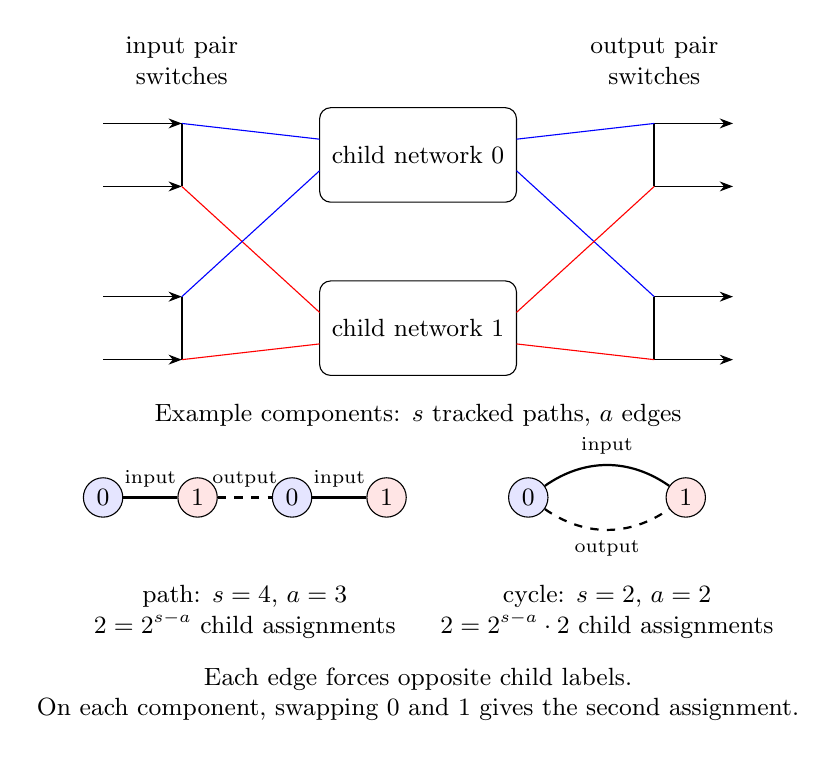
\begin{tikzpicture}[x=1cm,y=1cm,>=Stealth,font=\small]
\node[draw,rounded corners,minimum width=2.5cm,minimum height=1.2cm] (a) at (0,1.1) {child network $0$};
\node[draw,rounded corners,minimum width=2.5cm,minimum height=1.2cm] (b) at (0,-1.1) {child network $1$};
\foreach \y in {1.5,.7,-.7,-1.5}{
 \draw[->] (-4,\y)--(-3,\y);
 \draw[->] (3,\y)--(4,\y);
}
\draw[thick] (-3,1.5)--(-3,.7);
\draw[thick] (-3,-.7)--(-3,-1.5);
\draw[thick] (3,1.5)--(3,.7);
\draw[thick] (3,-.7)--(3,-1.5);
\draw[blue] (-3,1.5)--(-1.25,1.3);
\draw[red] (-3,.7)--(-1.25,-.9);
\draw[blue] (-3,-.7)--(-1.25,.9);
\draw[red] (-3,-1.5)--(-1.25,-1.3);
\draw[blue] (1.25,1.3)--(3,1.5);
\draw[blue] (1.25,.9)--(3,-.7);
\draw[red] (1.25,-.9)--(3,.7);
\draw[red] (1.25,-1.3)--(3,-1.5);
\node[align=center] at (-3,2.3) {input pair\\switches};
\node[align=center] at (3,2.3) {output pair\\switches};

\begin{scope}[
 tracked/.style={circle,draw,minimum size=5mm,inner sep=0pt},
 child zero/.style={tracked,fill=blue!10},
 child one/.style={tracked,fill=red!10},
 input constraint/.style={thick},
 output constraint/.style={thick,dashed}
]
\node at (0,-2.2) {Example components: $s$ tracked paths, $a$ edges};
\node[child zero] (p0) at (-4,-3.25) {$0$};
\node[child one]  (p1) at (-2.8,-3.25) {$1$};
\node[child zero] (p2) at (-1.6,-3.25) {$0$};
\node[child one]  (p3) at (-.4,-3.25) {$1$};
\draw[input constraint] (p0)--node[above,font=\scriptsize] {input} (p1);
\draw[output constraint] (p1)--node[above,font=\scriptsize] {output} (p2);
\draw[input constraint] (p2)--node[above,font=\scriptsize] {input} (p3);
\node[child zero] (c0) at (1.4,-3.25) {$0$};
\node[child one]  (c1) at (3.4,-3.25) {$1$};
\draw[input constraint] (c0) to[bend left=35]
 node[above,font=\scriptsize] {input} (c1);
\draw[output constraint] (c0) to[bend right=35]
 node[below,font=\scriptsize] {output} (c1);
\node[align=center] at (-2.2,-4.7)
 {path: $s=4$, $a=3$\\$2=2^{s-a}$ child assignments};
\node[align=center] at (2.4,-4.7)
 {cycle: $s=2$, $a=2$\\$2=2^{s-a}\cdot 2$ child assignments};
\node[align=center] at (0,-5.75)
 {Each edge forces opposite child labels.\\On each component, swapping $0$ and $1$ gives the second assignment.};
\end{scope}
\end{tikzpicture}

\caption{A recursive network node (top) and two components of a routing-constraint graph (bottom). Each graph vertex represents a tracked path, and each input or output edge forces its endpoints into opposite children. Both displayed components have two child assignments, but the cycle contributes an extra factor $2$ relative to $2^{s-a}$. The four paths in the network panel are schematic; each child contains half the positions.}
\label{fig:network-node}
\end{figure}

Each assignment prescribes $2s-a$ independent outer coins, hence costs $2^{-(2s-a)}$. Their combined factor is $2^{-s+C}$. Recursing through the nodes and choosing proper colorings uniformly gives a density relative to the uniform injection with excess exponent
\begin{equation}\label{net:exponent}
 X=\sum_{j=1}^d C_j+\log_2\frac{(N)_k}{N^k},
\end{equation}
where $C_j$ totals tracked cycles at height $j$. We distinguish the auxiliary coloring law from the actual switch law. For fixed input and output injections $x,y$, let $\omega$ be a legal complete tree of child colorings. At a node $v$, write $s_v,e_v,C_v$ for its path, edge and cycle counts, and put $a_v=2^{s_v-e_v+C_v}$. The auxiliary weight and actual routing-event weight are respectively
\[
 q_{xy}(\omega)=\prod_v a_v^{-1},\qquad
 w_{xy}(\omega)=\prod_v2^{-(2s_v-e_v)},\qquad
 \frac{w_{xy}(\omega)}{q_{xy}(\omega)}
      =N^{-k}2^{\sum_vC_v}.
\]
The last identity uses $\sum_vs_v=kd$. At the leaves the routing is determined. Summing unused switch coins contributes one, so $w_{xy}(\omega)$ is exactly the probability of the corresponding endpoint-and-coloring event. Thus
\[
 K_N(x,y)=\sum_\omega w_{xy}(\omega)
       =\frac1{(N)_k}\E_{q_{xy}}2^X.
\]
For the certificate alternative in Section~\ref{sec:certificate}, one may truncate the routing event itself. Define $A(x,y)=\sum_\omega w_{xy}(\omega)\mathbf1_{\{X\le L\}}$ and $E=K_N-A$. Then $A(x,y)\le2^L/(N)_k$, while
\begin{equation}\label{net:discarded-actual-law}
 \sum_y E(x,y)=\sum_{y,\omega}w_{xy}(\omega)\mathbf1_{\{X>L\}}
             =\PP_{\mathrm{actual},x}(X>L).
\end{equation}
Indeed $(y,\omega)$ partitions the actual switch experiment. The tail estimates below therefore bound discarded mass under the actual network law, without identifying that law with the auxiliary uniform-coloring law. The factor $(N)_k/N^k$ is essential: the endpoints form an injection, not a tuple sampled with replacement.

\begin{lemma}[Truncation and repeated irreducible copies]\label{net:truncation}
Let a finite group act transitively on a set of size $M$, and let $Q$ be the symmetric Markov kernel induced on its permutation module by a probability measure on that group. Suppose $Q=A+E$ entrywise, where $A,E\ge0$, every entry of $A$ is at most $B/M$, and the row and column sums of $E$ are at most $p$. If an irreducible representation occurs with multiplicity $m>0$, then
\[
 \|Q(\lambda)\|_{\op}\le \sqrt{B/m}+p.
\]
It is not necessary that $A$ preserve the irreducible subspaces.
\end{lemma}
\begin{proof}
Schur's test gives $\|E\|_{\op}\le p$. Since the row sums of $A$ are at most one,
$\|A\|_{\HS}^2\le(B/M)\sum_{x,y}A(x,y)\le B$.
Choose one maximizing unit vector for $Q(\lambda)$ in each of its $m$ orthogonal equivalent copies. They are orthonormal and each image under $A$ has norm at least $\|Q(\lambda)\|_{\op}-p$. Their squared image norms sum to at most $\|A\|_{\HS}^2$. This proves the claim.
\end{proof}
The first proof in Section~\ref{sec:factorial} instead truncates the endpoint density: it retains an entry when $(N)_kK_N(x,y)\le z$. Its density moment bounds the discarded row mass by Markov's inequality, and symmetry bounds the column mass. Both cutoffs use Lemma~\ref{net:truncation}; the letter $Q$ in that abstract lemma denotes any kernel satisfying its hypotheses.

For the routing-event cutoff above, reversal preserves the cutoff event, so a uniform discarded-row bound also bounds columns. Lemma~\ref{net:truncation} therefore gives $2^{L/2}/\sqrt m+p$.


\subsection{How often can selected paths meet?}
The next deterministic fact will control the information revealed about a closing route by other paths. Its logarithm is to base two.
\begin{lemma}[Butterfly encounters]\label{net:encounters}\label{n:butterfly-contacts}
Any $h$ distinct routed paths through a butterfly that updates each of $d$ binary coordinates once have at most $h\log_2h/2$ shared switches in total, with $0\log_2 0=0$. Their contact graph has maximum degree at most $d$. Counting both path endpoints at each shared switch gives at most $h\log_2h$ contacts.
\end{lemma}
\begin{proof}
Split by the coordinate edited last. If the two classes have sizes $a,h-a$, that layer contributes at most $\min(a,h-a)$ meetings. Apply induction to the earlier subnetworks and use
\[
 2\min(a,h-a)\le h\log_2h-a\log_2a-(h-a)\log_2(h-a).
\]
This is the binary entropy inequality $H_2(x)\ge2\min(x,1-x)$, where $H_2(x)=-x\log_2x-(1-x)\log_2(1-x)$. Empty terms are zero. Summing over the recursive splits proves the assertion. Distinct paths meet at most once: after a common switch they differ in a coordinate that is never edited again. A path meets at most one other path at each of its $d$ switches, proving the degree assertion.
\end{proof}


\section{The factorial-moment proof}\label{sec:factorial}
We now prove Theorem~\ref{fac:main}. The cycle estimate controls sparse injections and very large representation dimensions. The remaining dimensions require a second density estimate, obtained after replacing fixed-size middle blocks by uniform permutations. We prove both density assertions before making the representation split.

For the recursive description number the coordinates so that the palindrome uses layers $d,\ldots,1,1,\ldots,d$. A node of size $2^t$ varies in its low $t$ coordinates. This reversal of coordinate names does not change its law up to conjugation. Thus $K_N=T_N^*T_N$, consistently with Section~\ref{sec:introduction}, and $\|K_N(\lambda)\|=\|T_N(\lambda)\|^2$.

\subsection{Closing routes and factorial cycle moments}
An alternating cycle in the network can be followed by going through one
child and returning through the other. After one child map is fixed, this
produces a permutation containing fresh butterfly layers between fixed
bijections. The following lemma counts several cycles of such a
permutation at once. Its distinguished slots let us sum over all choices
of cycle lengths without losing a factorial.

\begin{lemma}[Factorial moments with distinguished cycle slots]\label{fac:cycle-factorial}
On a finite set take a permutation given by independent butterflies of block size $n=2^r$ in parallel, composed before and after with arbitrary fixed permutations (we allow identifications of the sets at each stage). Fix a subset of size at most $k$, and count cycles lying entirely inside it, with $F_j$ the number of length $j$. For nonnegative integers $a_j$ (finitely supported) and $A=\sum a_j$,
\begin{equation}
\mathbb E\prod_j(F_j)_{a_j}\ \le\ (k/\sqrt n)^A\prod_j j^{-a_j/2}.
\label{fac:e3}
\end{equation}
Here $(F)_a=F(F-1)\cdots(F-a+1)$ and $(F)_0=1$.
\end{lemma}
\begin{proof}
Order the sought cycles by nondecreasing length, with slots distinguished, and choose a starting vertex for each (at most $k^A$ choices). Following a cycle involves querying successive butterfly paths, with the last one required to close the cycle. Demand that these are the specified lengths with no repetitions before closure, are disjoint cycles, and are within the subset; otherwise call this failure. Each closing path has a specified input and output by the time it needs to be queried; conditional on the previous path exposures its probability is zero or $2^u/n$, where $u$ counts switches on that route already exposed (a route through a single butterfly to a given compatible endpoint is unique). If $\mathcal G$ is the exploration just before a closing query, its
required input and output are $\mathcal G$-measurable, and
\[
 \E[\mathbf1_{\{\mathrm{closure}\}}n2^{-u}\mid\mathcal G]\le1,
\]
with value zero for an incompatible route. Ordinary nonclosing queries
insert no weight. Iterating these conditional identities, while
requiring all the distinctness and length conditions, gives
\[
\mathbb E[1_{\rm success} n^A 2^{-U}]\le 1
\]
for each choice of starts, with $U$ the sum of those counts on success. This follows also by sequentially forcing the closing paths when possible, which changes measure by the indicated factors while other path steps cost no weight.

It remains to bound how much the previously exposed paths can help the closing routes. For a realized collection in specified slots, rotate its starts independently uniformly. $U$ counts meetings of selected butterfly paths, namely when the closing path uses a switch met previously. Weight each selected path in a cycle of length $j$ by $1/j$. For meetings between different cycles the expected charge per meeting over rotations is the smaller of the weights (or bounded by it), since cycles are processed by length. Within one cycle it is at most $2/j$. For any subset of $s$ selected paths the total meetings between them in a butterfly layer sequence is at most $sr/2$. Within paths of one cycle of length $j$, Lemma~\ref{net:encounters}
gives the stronger bound $j\log_2j/2$. For several independent
butterfly blocks, apply the lemma in each block and use
$\sum_i j_i\log j_i\le j\log j$ when $\sum_i j_i=j$.
Now integrate the subset bound $sr/2$ over thresholds on the weights: this gives $Ar/2$ for the sum charging each meeting the minimum weight. The additional within-cycle charges give at most $\sum_j a_j\log_2(j)/2$. By Jensen, the sum over rotations ($\prod_j j^{a_j}$ of them) of $2^{-U}$ for each collection is thus at least
\[
\prod_j j^{a_j}\, n^{-A/2}\prod_j j^{-a_j/2}.
\]
To make the counting explicit, let $\mathfrak C(\omega)$ be the set of ordered collections of distinct cycles of the realized permutation, with $a_j$ distinguished slots of length $j$. Its cardinality is $\prod_j(F_j(\omega))_{a_j}$. Each collection has exactly $\prod_jj^{a_j}$ choices of starts. Sum the weighted success inequality over all start choices, then interchange that sum and the expectation. The preceding lower bound for the total rotation weight gives
\[
 k^A\ge \E\sum_{\mathcal C\in\mathfrak C(\omega)}
             \sum_{\text{starts of }\mathcal C} n^A2^{-U}
 \ge n^{A/2}\prod_jj^{a_j/2}\,
              \E\prod_j(F_j)_{a_j}.
\]
Dividing proves \eqref{fac:e3}.
\end{proof}

For later use, if $q\ge1$ and $J\ge1$ is an integer, cycles longer than $J$ contribute at most $k/J$. Expanding $q^{\sum_{j\le J}F_j}$ in factorial moments and using $\sum_{j\le J}j^{-1/2}\le2\sqrt J$ gives
\begin{equation}
\log \mathbb E q^{\sum_j F_j}\le (k/J)\log q+2q k\sqrt J/\sqrt n .
\label{fac:e4}
\end{equation}

\subsection{The two density estimates}\label{net:factorial-route}
\begin{lemma}[Palindromic row-density moments]\label{fac:density}
Let $N=2^d$, $1\le k\le N$, and $a=1/1000$. For a kernel $Q$ on ordered $k$-injections define
\[M(Q,k)=\sup_{x\in\mathcal X_{N,k}}\E_{y\sim u_{N,k}}\big[(N)_kQ(x,y)\big]^{1+a}.\]
There are absolute $C,\eta>0$ with the following properties; below $M$ denotes $M(Q,k)$ for the kernel in question.
\begin{itemize}
\item for $K_N$, $\log M\le C k(k/N)^{\eta}$, for some absolute $C<\infty$ and $\eta>0$;
\item consider the modified palindrome obtained by replacing the central subnetworks of size $S=2^L$ by independent uniform permutations, except in at most $b$ specified such blocks where they are replaced by identity. For every $\xi>0$, there is $L_0$ such that for each fixed $L\ge L_0$ there are $\epsilon>0$ and $d_0\ge L$ for which $M(Q,N)\le e^{\xi N}$ whenever $d\ge d_0$ and $bS/N\le\epsilon$.

\end{itemize}\end{lemma}\begin{proof}
For $N=1$, the only injection has one position and every kernel in the
statement is identity, so $M=1$. Assume henceforth that $d\ge1$.
To see how to estimate these integrals, expand the transition probability by splitting off the outermost layers of each block, recursively. At a given node of size $2^t$, let $h$ be the number of marked paths (the paths of the tuple) there. Given their endpoints at that node, write $b_x,b_y$ for the numbers of occupied direction-$t$ pairs at the two ends. Each term assigns each path to one of the two children, with opposite assignments for a pair coming from the same direction-$t$ edge on either end. Its probability factor for the outer layers is $2^{-b_x-b_y}$. On the labels of paths the two matchings (allowing unmatched vertices) giving these constraints form alternating chains and even cycles, counting parallel matching edges as a cycle as well. If there are $z$ cycles the number of assignments is at most $2^{b_x+b_y-h+z}$, by counting components. Each assignment fixes the child endpoints, and has as further factors the child probabilities. Apply
\[
(\sum_i p_i)^{1+a}\le (\# i)^a\sum_i p_i^{1+a}
\]
at each expansion. On summing over terminal tuple images $y$, keeping one power of each term as the actual routing probability, the remaining factors at expanded nodes give $2^{a(-h+z)}$. Thus, for any initial tuple,
\begin{equation}
\E_{y\sim u_{N,k}} R_x(y)^{1+a}
 \le [(N)_k/N^k]^a\,\mathbb E 2^{a\sum_{t=1}^d Z_t},
\label{fac:e1}
\end{equation}
where $Z_t$ totals the cycles at level $t$ of the actual routing (unused paths can be filled in via the actual switches). For the modified palindrome with $k=N$, stop after levels $d,\ldots,L+1$. Instead the bound is
\begin{equation}
[N!\,(S/N)^N (S!)^{-N/S+b}]^a\,\mathbb E 2^{a\sum_{t>L} Z_t}.
\label{fac:e2}
\end{equation}
Indeed all paths are then used and the extra central probability factors are uniform $(S!)^{-1}$ or identity.

\medskip\noindent\textbf{Fresh layers at one height.}\enspace
Lemma~\ref{fac:cycle-factorial} concerns fresh butterfly layers, whereas
cycle counts at different network heights share coins. Label paths at the
central cross section and read the two butterflies outward, calling them
$X$ and $Y$. Conditioning on $X$ fixes the marked central labels.

Fix a height $t$. Let $\Omega_0,\Omega_1$ be the unions of the bit-zero
and bit-one halves in direction $t$ of all size-$2^t$ nodes. Reading the
first $t-1$ layers of $X$ gives bijections $X_0,X_1$ from these halves to
a common set of switch columns. The input matching, viewed from
$\Omega_0$ to $\Omega_1$, is $I=X_1^{-1}X_0$. The corresponding output
matching is $Y_1^{-1}Y_0$. Hence following an output edge and then an input
edge gives the permutation
\begin{equation}\label{fac:relative-permutation}
 \pi_t=I^{-1}Y_1^{-1}Y_0
       =X_0^{-1}X_1Y_1^{-1}Y_0
       \quad\hbox{on }\Omega_0.
\end{equation}
Each full alternating cycle gives one cycle of $\pi_t$.
The tracked count $Z_t$ includes only those cycles whose vertices on both
sides are marked. In particular it is bounded by the number of cycles of
$\pi_t$ contained in the marked subset of $\Omega_0$, a fixed set of
size at most $k$ under the conditioning on $X$. Switches at layer $t$
change neither matching.

Now expose the first $s<t-1$ outward layers of $Y$, and, for this
single-height estimate, the remaining maps on $\Omega_1$. The map $Y_1$
is then fixed. On $\Omega_0$, write $Y_0=B U$, where $U$ is the exposed
map through height $s$ and $B$ consists of fresh parallel butterflies in
coordinates $s+1,\ldots,t-1$, each of size $n=2^{t-1-s}$. Thus
$\pi_t=(I^{-1}Y_1^{-1})B U$ has exactly the form of
Lemma~\ref{fac:cycle-factorial}. Its bound is uniform in the exposed
maps, so it remains valid after averaging the extra exposure of $Y_1$.

\medskip\noindent\textbf{Summing heights with their conditioning.}\enspace

Here and below group levels above some integer $H\ge1$ into slabs
\[
l<t\le 2l,\qquad l=H,2H,4H,\ldots
\]
cut off at $d$. Put $\mathcal F_s=\sigma(X,\text{the first $s$ outward layers of }Y)$ and
$B_l=\sum_{l<t\le\min(2l,d)}Z_t$. The band variable $B_l$ is
$\mathcal F_{2l}$-measurable (with $\mathcal F_s=\mathcal F_d$ for $s>d$).
Split the slabs into their two alternating families. In either family,
the preceding slab ends at $l/2$, so its cycle count is
$\mathcal F_{\lfloor l/2\rfloor}$-measurable.

Conditioned on that field, the single-level estimate above has a fresh
butterfly of size $n\ge2^{l/2}$. H\"older within the slab uses at most
$l$ factors. For the exponential moment with exponent $2a$, take
$q=2^{2al}$ and $J=\lceil2^{l/16}\rceil$ in \eqref{fac:e4}. Uniformly in
the conditioning,
\begin{equation}
\log\E[q^{Z_t}\mid\mathcal F_{\lfloor l/2\rfloor}]
 \le Ck2^{-c_0l}.
\label{fac:e5}
\end{equation}
The two terms on the right of \eqref{fac:e4} decay exponentially because
$2a<1/16$. Thus, after H\"older,
\[
 \E[2^{2aB_l}\mid\mathcal F_{\lfloor l/2\rfloor}]
 \le\exp(Ck2^{-c_0l}).
\]
For example, if $l_*$ is the last slab in one family and $V$ is the sum
of its earlier bands, the tower property gives
\[
 \E[2^{2a(V+B_{l_*})}\mid X]
 =\E\!\left[2^{2aV}
   \E[2^{2aB_{l_*}}\mid\mathcal F_{\lfloor l_*/2\rfloor}]
   \,\middle|\,X\right]
 \le e^{Ck2^{-c_0l_*}}\E[2^{2aV}\mid X].
\]
Iterate backwards through each family and apply Cauchy--Schwarz to the
two families. The geometric sum of their costs proves
\begin{equation}
\log\E[2^{a\sum_{t>H}Z_t}\mid X]\le Ck2^{-c_1H}.
\label{fac:e6}
\end{equation}
The same reasoning holds with $a$ replaced by $2a$: even the resulting
single-level exponent $4a$ is smaller than $1/16$. We will use this
explicit doubling when separating low and high levels.

\medskip\noindent\textbf{Low heights and the sparse density bound.}\enspace
The high-height cost decays with its starting height. At low heights, sparse occupancy supplies the gain instead. For the low levels of \eqref{fac:e1}, partition the central labels into size $R=2^H$ blocks and let $V_D$ count marked positions in such a block $D$. (Use $H\le d$.) All low-level cycles are internal to such blocks and
\[
\sum_{t\le H} Z_t\le H\sum_D V_D 1_{V_D\ge2}.
\]
For every set of central positions of size $v$ the probability under $X$ they are all marked is at most $p^v$, $p=k/N$. Indeed the upper product-of-marginals bound for every subset holds initially (trace the marked inputs towards the center). It is preserved under a single fair switch: for sets with one endpoint use averaging of the two bounds; with both endpoints use the old product, bounded by the product with both marginals replaced by their mean. After the layers of $X$ each position has marginal $p$.

Write $w=2^{aH}$. In each block use
\[
w^{V_D 1_{V_D\ge 2}}\le 1+\sum_{i=2}^{R}{V_D\choose i} w^i.
\]
Expanding the product and using the joint inclusion bounds yields
\[
\log\mathbb E 2^{a\sum_{t\le H} Z_t}
\le (N/R)\sum_{i=2}^{R}{R\choose i}(p w)^i
\le C(N/R)(R p w)^2
\]
when $Rpw$ is bounded. Choose
$H=\max(1,\lfloor\log_2(1/p)/4\rfloor)$; then $H\le d$.
For the low-height estimate with exponent $2a$, replace $w$ by
$2^{2aH}$. The product $Rp w$ stays bounded, and the resulting logarithmic
cost is at most
\[
 Ck p R2^{4aH}\le C'k p^{(3-4a)/4}.
\]
The high-height estimate \eqref{fac:e6} also holds at exponent $2a$,
with cost at most $Ck2^{-c_1H}$. Low heights still depend on $Y$, so use
Cauchy--Schwarz between the two height ranges, then average over $X$.
Their costs are at most $Ck p^\eta$ for some absolute $\eta>0$.
The normalization in \eqref{fac:e1} is at most one, proving the first
claim. If there are no heights above $H$, only the low-height bound is
needed.

\medskip\noindent\textbf{Uniform central blocks and the dense density bound.}\enspace
For \eqref{fac:e2}, label paths at the input boundary of the central
size-$S$ blocks. Fix the input-side outer butterfly $X$, and include the
uniform or identity central maps at the beginning of $Y$. Use the same
slabs with $H=L$. We distinguish their first members, $l=L$ and $l=2L$,
from the later ones.

At a later slab, $l\ge4L$, condition on $X$, the central maps, and the
ordinary output layers through height $\lfloor l/2\rfloor$. The previous
same-parity slab is measurable in this field. All fresh coordinates used
in \eqref{fac:e5} lie strictly above the central blocks, so that estimate
applies unchanged with $k=N$.

A first slab has no preceding member in its parity family. We therefore
need its moment only conditional on $X$, without fixing the central
permutations. For a height $t$ in this slab expose the bit-one map as in
\eqref{fac:relative-permutation}. In each good bit-zero central block,
realize its uniform permutation as $F U$, where $U$ is an independent
uniform permutation and $F$ is an independent fresh size-$S$ butterfly.
This has the original uniform law. Condition on $U$, but leave $F$ fresh.
In a bad block take $U$ to be identity; the original central map there
is identity. In a comparison experiment insert a fresh $F$ in that block
too, keeping all good-block maps and all later switches the same.

Here is why this insertion costs at most $bS$ cycles. Let $B$ be the
union of the bad block inputs in the fresh-map coordinates. The original
and comparison maps agree on every input outside $B$. After any fixed
premap $U$, the affected domain is $U^{-1}B$, still of size at most $bS$;
a fixed postmap does not enlarge that domain. Every cycle of the
original relative permutation disjoint from $U^{-1}B$ retains all its
arrows and is therefore a cycle of the comparison permutation. At most
$bS$ disjoint cycles meet that domain. Thus, writing $Z'_t$ for the full
comparison cycle count,
\[
 Z_t\le Z'_t+bS.
\]
This comparison holds for every realization of the inserted switches;
no cycle is selected for subsequent conditioning.

In the comparison, the central butterflies and the ordinary output
layers together form fresh parallel butterflies in coordinates
$1,\ldots,t-1$, between fixed maps. Lemma~\ref{fac:cycle-factorial}
therefore bounds their cycle moment. With $q=2^{2al}$, the same choice
$J=\lceil2^{l/16}\rceil$ as before gives, after averaging the auxiliary
maps,
\[
 \log\E[q^{Z_t}\mid X]
 \le CN2^{-c_0l}+bS\log q
 \qquad(l=L\hbox{ or }2L).
\]
H\"older within this first slab costs $O(a l bS)$ in addition to its
decaying term. Integrate the later slabs backwards in each parity family
using their lower-height conditioning, finish with this first-slab
bound, and apply Cauchy--Schwarz between the families. The result is
\[
 \log\mathbb E 2^{a\sum_{t>L}Z_t}
 \le C N 2^{-c_1 L} + C a L bS .
\]
By Stirling, the logarithm of the normalization in square brackets in
\eqref{fac:e2} is at most
$O(\log N+N\log S/S)+b\log(S!)$. Given $\xi>0$, first take $L$
large enough that the terms $N2^{-c_1L}$ and $N\log S/S$ have sufficiently
small coefficients. With that $L$ fixed, choose $\epsilon$ so that
$bS/N\le\epsilon$ controls both bad-block terms, and finally take $d$
large enough to absorb $O(\log N)$. This proves the second claim in the
stated order of choices.
\end{proof}

\subsection{Multiplicity amplification and the middle dimension range}
We now use the branching multiplicity from
\eqref{eq:tuplemultiplicity}: the ordered $k$-injection module contains
$\lambda\vdash N$ with multiplicity $m=f^{\lambda/(N-k)}$, and for
$k=N$ this is $D_\lambda$. The density bounds just proved will make
truncation effective on these repeated copies.

For either symmetric kernel $Q$ above, retain an entry when its density
is at most $z$. Markov's inequality gives discarded row mass at most
$Mz^{-a}$, and symmetry gives the same column bound. The retained
entries are at most $z/(N)_k$. Applying
Lemma~\ref{net:truncation} with $B=z$ therefore gives, on an irreducible
occurring with multiplicity $m>0$,
\begin{equation}
 \|Q(\lambda)\|\le Mz^{-a}+\sqrt{z/m}.
 \label{fac:e7}
\end{equation}
In particular if $\log M\le (a/4)\log m$, take $z=\sqrt m$ to get at most $2m^{-a/4}$.

First consider $j=N-\lambda_1$ with $1\le j\le\delta N$, where a sufficiently small absolute $\delta>0$ will be used. Choose a fixed $u_0>0$ small enough that $\eta(1-u_0)>u_0$ and $u_0<1$, and take $k=\lceil j(N/j)^{u_0}\rceil$. For small $\delta$ this gives $N-k\ge j$, so the skew tableau of shape $\lambda/(N-k)$ has its remaining first row independent of the entire tail shape $\rho=(\lambda_2,\ldots)$. Consequently
\[
m=\binom{k}{j} f^\rho,\qquad D_\lambda\le \binom Nj f^\rho.
\]
Thus $\log m\ge u_0 j\log(N/j)+\log f^\rho$, at least a fixed positive fraction of $\log D_\lambda$ (using the elementary binomial bounds). The first density bound proved above gives $\log M\le C' j(j/N)^{\eta(1-u_0)-u_0}$, hence at most $(a/4)\log m$ by reducing $\delta$. By \eqref{fac:e7}, and $m$ tending uniformly to infinity here as $d\to\infty$, we have $\|K_N(\lambda)\|\le D_\lambda^{-c_2}$ for some constant $c_2>0$.

By Lemma~\ref{lem:annihilation}, shapes with more than $N/2$ rows
are annihilated by $T_N$ and hence by $K_N$.

All remaining shapes other than the trivial one and those already treated have $j\ge\delta N$ and
\[
\log D_\lambda\ge hN
\]
with $h>0$ fixed, for large $N$. Here are details. Both first row and column are then bounded by $(1-\delta)N$ (take $\delta<1/2$). If both are smaller than $N/10$, hook lengths are at most $N/5$ and the bound follows from Stirling. Otherwise transpose if necessary (which does not change dimension) so the row has length $s\ge N/10$. Retain only it and a subdiagram of the tail of size $v=\lfloor\min(\delta/2,1/100)N\rfloor$, which can be obtained by removing corners. All tableaux on this diagram have extensions. Fill its first $v$ positions in the top row first, then interleave the remaining row and a fixed tableau order on the tail; this gives $\binom{s}{v}$ possibilities, yielding the asserted exponential lower bound.

Take a fixed large $A_0$ so that when $\log D_\lambda\ge A_0 N$, the first density bound on all $N$ positions gives $\log M\le(a/4)\log D_\lambda$. Then \eqref{fac:e7} with $Q=K_N$ again gives $\|K_N(\lambda)\|\le D_\lambda^{-c_3}$ for an absolute $c_3>0$, for large $N$.

The only remaining range is $hN\le\log D_\lambda\le A_0 N$. Here the full-deck moment cost $CN$ is comparable with the log dimension and need not fit the truncation threshold. We use the modified central networks to reduce that cost before invoking multiplicity. Choose $L$ fixed sufficiently large and then $\epsilon>0$ sufficiently small so the second of the two assertions about the $(1+a)$-moment above gives $\log M\le ahN/4$ whenever $b\le\epsilon N/S$, for large $N$. We justify the comparison in positive semidefinite order. Let $O$ be
the product of the outer butterfly layers, and let $C$ be the parallel
product of the central size-$S$ palindrome operators. Thus, on the
representation under consideration,
\[
 K_N=O^*CO.
\]
By Lemma~\ref{lem:finitegap}, each central positive contraction has norm
at most a fixed $\theta<1$ on every nontrivial irreducible of $S_S$;
increase $\theta$ to a number in $(0,1)$ if necessary.

Restrict to $(S_S)^{N/S}$ and decompose into tensor-product irreducibles,
with their multiplicity spaces. If a component is nontrivial on more
than $\epsilon N/S$ blocks, the tensor product defining $C$ has norm at
most $\theta^{\epsilon N/S}$. This accounts for the first term below.

For $E\subseteq[N/S]$, let $P_E$ act as identity in blocks in $E$ and
as the projection to invariants in the other blocks. On a component
whose nontrivial factors lie in a set $F$ with $|F|\le\epsilon N/S$,
$P_F$ is identity. Consequently $\sum_{|E|\le\epsilon N/S}P_E$
dominates identity on all these components and therefore dominates
$C$ there. Its sandwich
\[
 Q_E=O^*P_EO
\]
is precisely the modified network with identity in $E$ and uniform
central permutations elsewhere. Since $O$ is a contraction, these two
component cases give
\[
0\le K_N(\lambda)\le \theta^{\epsilon N/S} I+\sum_{E:\, |E|\le\epsilon N/S}Q_E(\lambda)
\]
where $Q_E$ is exactly the modified palindrome with identity in $E$ and uniform central permutations elsewhere. Each summand by \eqref{fac:e7}, $k=N$, is at most $2D_\lambda^{-a/4}$ in norm. The log number of summands is at most $(N/S)[-\epsilon\log\epsilon-(1-\epsilon)\log(1-\epsilon)]$ by the binomial theorem ($\epsilon<1/2$), so we may require also that this be $\le ah N/8$. Since $hN\le\log D_\lambda\le A_0 N$ and all parameters now are fixed absolutely, this proves $\|K_N(\lambda)\|\le D_\lambda^{-c_4}$ for some absolute $c_4>0$ and sufficiently large $N$.

We have consequently, on every nontrivial shape not killed, $\|T_N(\lambda)\|\le D_\lambda^{-c_*}$ for an absolute $c_*>0$. Plancherel on the finite group and Cauchy-Schwarz bound four times the squared total variation distance after $r$ butterflies by
\[
\sum_{\lambda\ne (N)} D_\lambda\,\|T_N(\lambda)^r\|_{\rm HS}^2,
\]
independently of initial permutation by translation. For $r$ forward sweeps,
\[
 \|T_N(\lambda)^r\|_{\HS}^2
 \le D_\lambda\|T_N(\lambda)^r\|_{\op}^2
 \le D_\lambda\|T_N(\lambda)\|_{\op}^{2r}.
\]
Thus, keeping only shapes not killed, the sum is at most
$\sum D_\lambda^{2-2rc_*}$.

This last bound tends to zero for sufficiently large fixed $r$. Medium or larger dimensions with $\log D_\lambda\ge hN$ have at most $2^N$ terms (bound partitions by compositions). For the small-$j$ range, $D_\lambda\ge \binom{N-j}{j}$: again fill $j$ positions of the first row first and then interleave tail and remaining row. There are at most $2^j$ shapes per $j$. Thus, with $s_*=2r c_*-2>0$, this range contributes at most
\[
\sum_{1\le j\le\delta N}2^j(j/(N-j))^{s_*j}
\]
tending to zero (choose $s_*$ large for a geometric summable majorant and each fixed term vanishes). Increase $r$ also so that $s_* h>\log 2$. Hence $rd$ steps suffice for the required threshold for all sufficiently large $d$.


\section{Certificate tails and numerical dense bounds}\label{sec:certificate}
The factorial proof is complete. This independent route keeps information that its central-block comparison does not: explicit bounds on the exponential density cost at fixed tracked-card densities. We first count fixed certificates for many short cycles, then estimate reciprocal cycle lengths and pass to all representation shapes. Here $n=2^d$ is the full-deck size and $r$ is the number of tracked cards. Thus the exponent in \eqref{net:exponent} is used with $N=n$ and $k=r$. Logarithms in this section are to base two unless $\ln$ is written.

\subsection{A fixed-certificate cycle tail}\label{net:certificate}
\begin{proposition}[High-height cycle tail]\label{net:hightail}
There are absolute $b,\delta>0$ and an integer $J_0\ge1$ such that, uniformly in the tracked input injection of size $r$ and for every integer $J\ge J_0$,
\begin{align}
 \log_2\E 2^{b\sum_{j\ge J}C_j}&\le O(r2^{-bJ}),\label{net:highmgf}\\
 \log_2\E 2^{b\sum_jC_j}&\le O(r(r/n)^\delta).\label{net:sparsemgf}
\end{align}
The first bound also holds with expectation conditional on all input-side
switches and all output switches of heights at most $s$, for every integer
$0\le s\le d$ with $2s<J$, uniformly in the fixed switch values and with
the same absolute implied constant.
\end{proposition}
\begin{proof}
The estimates are immediate for $r=0$, so assume $r\ge1$.
Let $\mathcal F_t$ be the sigma-field generated by all input-side
switches and the output switches of heights at most $t$.
The arrivals at every node are determined by the input switches.
At a height-$j$ node the two child maps determine its cycles; the
outer output switch only exchanges the two positions in an output
pair and does not change their pairing.  Thus $C_j$ is
$\mathcal F_{j-1}$-measurable.

Fix a nonnegative integer $t$ with $2t<j$ and condition on $\mathcal F_t$.
In each height-$j$ node expose one child's remaining switches.
In the other child the fixed low layers are followed by independent
parallel output butterflies of height $j-1-t$.  Since
$j-1-t\ge\lfloor j/2\rfloor$, at least
$m=\lfloor j/2\rfloor-1$ final output layers remain fresh.
This includes $t=(j-1)/2$ when $j$ is odd.
The two child bijections identify alternating cycles with cycles of
their relative permutation. Explore such a cycle through the fresh
child and back through the known inverse of the other. Its closing
target is specified, and the closing route through its remaining
butterfly is unique.

Suppose $C_j\ge s\ge r2^{-\eta j}$, where $\eta>0$ is a sufficiently small absolute constant. At least $s/2$ of some $s$ counted cycles have length at most $2r/s$. Among these choose $u=\max(1,\lfloor s/100\rfloor)$ cycles uniformly without replacement and choose a uniform cyclic start on each. A fresh-layer switch of a closing path meets at most one path of another cycle. The conditional chance of selecting that other short cycle is at most $(u-1)/(s/2-1)$, less than $1/49$ when $u>1$, and zero when $u=1$. Here we bound interference against all other selected cycles, including those later in the canonical exploration order; restricting to already explored cycles only decreases it. Thus mean cross-cycle interference on a closing path is less than $j/30$. Within its own cycle, Lemma~\ref{net:encounters} bounds the mean number of earlier encountered switches by $\log_2(2r/s)\le1+\eta j$. For large $j$, the expected total previously exposed switches on all closing paths is less than $uj/4$.

Consequently each realized network in this event admits a certificate of starts and lengths with at most $uj/4$ previously exposed closing switches. This is an existence assertion before taking a union bound; we do not condition the coin law on the chosen favorable cycles. There are at most
\[
 \binom ru(2r/s)^u
\]
fixed certificates. Order their starts canonically and explore each fixed certificate in that order. Define its success event to require that all prescribed cycles close and that at least $K=\lceil u(j/4-2)\rceil$ closing queries are fresh. The preceding low-interference existence argument supplies a certificate in this event for every network being counted. At every fresh closing query its required bit is already determined, so the query succeeds with conditional probability $1/2$, irrespective of intervening nonclosing queries. Abort if a closing bit fails or the certificate becomes invalid, and stop on the $K$th successful fresh closing query. The probability of reaching this stopping threshold without failure is at most $2^{-K}\le2^{-u(j/4-2)}$. This bounds the stated success event even when unsuccessful explorations make fewer than $K$ fresh queries. The base-two logarithm of the certificate count is at most
\[
 u\{\log_2(200er/s)+\log_2(2r/s)\}\le u(O(1)+2\eta j).
\]
Since $u\ge s/200$, reducing $\eta$ gives
$\PP(C_j\ge s\mid\mathcal F_t)\le2^{-cjs}$, uniformly in the
conditioning whenever $2t<j$.

Split the moment tail at $r2^{-\eta j}$. The deterministic part costs
$O(jr2^{-\eta j})$ and the remaining geometric tail is summable at
any sufficiently small fixed exponent. Decreasing that exponent
gives absolute $b',A>0$ and $J_0$ such that, for every $j\ge J_0$
and $2t<j$,
\begin{equation}\label{net:single-height-conditional}
 \log_2\E\bigl[2^{b'jC_j}\mid\mathcal F_t\bigr]
 \le Ar2^{-b'j}.
\end{equation}

We retain the conditioning while summing over heights. Fix integers
$J\ge J_0$ and $0\le s\le d$ with $2s<J$. If $J>d$, the
sum is empty. Otherwise put $L_q=2^qJ$ and, for each $q\ge0$
with $L_q\le d$, define
\begin{gather*}
 I_q=\{L_q,\ldots,\min(2L_q-1,d)\},\qquad
 B_q=\sum_{j\in I_q}C_j,\\
 \ell_q=|I_q|,\qquad
 t_q=\left\lfloor\frac{L_q-1}{2}\right\rfloor.
\end{gather*}
These bands partition the integer heights from $J$ to $d$.
We have $s\le t_q$, $2t_q<L_q$, and $\ell_q\le L_q$.
Choose $0<b\le b'/2$. Conditional H\"older within a band and
$2b\ell_q\le b'j$ for every $j\in I_q$ give
\begin{align*}
 \log_2\E\bigl[2^{2bB_q}\mid\mathcal F_{t_q}\bigr]
 &\le\frac1{\ell_q}\sum_{j\in I_q}
       \log_2\E\bigl[2^{2b\ell_q C_j}\mid\mathcal F_{t_q}\bigr]\\
 &\le\frac{Ar}{\ell_q}\sum_{j\in I_q}2^{-b'j}
 \le Ar2^{-b'L_q}.
\end{align*}

Split the band indices into their two parity classes, and let
$V_q=\sum_{p<q,\ p\equiv q\ (2)}B_p$.
For $q\ge2$, every earlier band in the same class ends at or
below $L_q/2-1\le t_q$. Since $C_j$ is
$\mathcal F_{j-1}$-measurable, $V_q$ is
$\mathcal F_{t_q}$-measurable; for $q=0,1$ it is zero.
Also $\mathcal F_s\subseteq\mathcal F_{t_q}$ for every band.
The conditional tower step is therefore
\begin{align*}
 \E\bigl[2^{2b(V_q+B_q)}\mid\mathcal F_s\bigr]
 &=\E\left[2^{2bV_q}
       \E\bigl[2^{2bB_q}\mid\mathcal F_{t_q}\bigr]
       \,\middle|\,\mathcal F_s\right]\\
 &\le 2^{Ar2^{-b'L_q}}
       \E\bigl[2^{2bV_q}\mid\mathcal F_s\bigr].
\end{align*}
Integrating the highest band first and then descending gives,
for $\varepsilon\in\{0,1\}$,
\[
 \E\left[2^{2b\sum_{q\equiv\varepsilon\ (2)}B_q}
       \,\middle|\,\mathcal F_s\right]
 \le 2^{Ar\sum_{q\equiv\varepsilon\ (2)}2^{-b'L_q}}.
\]
All band sums here are finite. Conditional Cauchy--Schwarz between
the two classes now yields
\[
 \log_2\E\left[2^{b\sum_{j\ge J}C_j}
       \,\middle|\,\mathcal F_s\right]
 \le\frac{Ar}{2}\sum_{q\ge0}2^{-b'2^qJ}
 \le A'r2^{-bJ}
\]
with an absolute $A'$. This proves the asserted conditional bound;
averaging it proves~\eqref{net:highmgf}. No independence between
different heights or bands has been assumed.

For \eqref{net:sparsemgf}, put $\rho=r/n$ and take $J=\lfloor .1\log_2(1/\rho)\rfloor$, or a fixed sufficiently large minimum. Below this height dominate cycles by shared input pairs. A law on occupancy bits is called strongly Rayleigh if its multiaffine generating polynomial has no zero when all variables have positive imaginary part. The deterministic occupancy law has a monomial generating polynomial. Fair transpositions preserve this property, and strongly Rayleigh laws are negatively associated: products of increasing functions on disjoint supports have expectation at most the product of their expectations~\cite[Theorems~4.9 and~4.20]{BorceaBrandenLiggett2009}. This is a fixed input-layer process, with no additional path conditioning. Indicators that both sites in a disjoint pair are marked are increasing functions on disjoint supports and inherit negative association. Their exponential moment is bounded by the product of the Bernoulli moments. A site's marginal before height $j$ is at most $2^j\rho$, and the two pre-switch input groups are independent because that coordinate has not yet been used. The expected number of shared pairs is therefore at most $r2^j\rho$. H\"older over the low heights introduces an exponent $O(J)$; decreasing the fixed $b$ if necessary, its cost is a positive power of $\rho$ times $r$.

The low-height dominating factor depends only on the input switches.
Conditioning on $\mathcal F_0$, pull that factor outside the
expectation and apply the uniform conditional high-height bound just
proved with $s=0$. Averaging over the input switches combines the
two costs and gives~\eqref{net:sparsemgf} for some absolute
$\delta>0$. This final estimate uses the input randomness.
If $\rho$ is bounded below, the fixed low heights cost $O(r)$,
which is consistent with~\eqref{net:sparsemgf} after changing the constant.
\end{proof}

\subsection{Dense tuple densities}\label{net:dense}
The sparse moment estimate alone does not provide a useful exponent at fixed density. Here a bound on reciprocal cycle lengths gives a smaller explicit density exponent. Define
\[
 h_j=\max\left\{\E(1/L):L\in\mathbb Z_{\ge1},\ \PP(L=l)\le l/2^{j-1}\right\},
\]
and
\[
 H(\rho)=\max\left\{\frac12\sum_{j\ge1}h_jx_j:
 0\le x_j\le1,\ \sum_{j\ge1}2^{-j}x_j\le\rho\right\}.
\]
\begin{proposition}[Dense truncation]\label{net:densetruncation}
For every $\rho_0\in(0,1]$ and $\epsilon>0$, there are
$c>0$ and $n_0$ such that, for every dyadic $n\ge n_0$ and
every integer $r$ with $\rho=r/n\in[\rho_0,1]$, the density
exponent \eqref{net:exponent} exceeds
\[
 r\left[H(\rho)+\frac{-\rho-(1-\rho)\ln(1-\rho)}{\rho\ln2}+\epsilon\right]
\]
with probability at most $\exp(-cr)$, uniformly in the input injection.
The constants depend only on $\rho_0,\epsilon$, and the expression
is interpreted continuously at $\rho=1$.
\end{proposition}
\begin{proof}
We first estimate the reciprocal length of a cycle in the relative
permutation of the two children at a height-$j$ node.  Put
$M=2^{j-1}$.  Fix one child's map and the other child's input-side
map, leaving its final output butterfly fresh.  Start at a uniform
boundary column.  For a proposed cycle length $l$, expose the first
$l-1$ edges.  The closing route is unique if compatible, and if $v$
of its switches have already been exposed, its conditional closing
probability is $2^v/M$.  Hence
\[
 \E[\ind_{\{L=l\}}2^{-v}]\le M^{-1}.
\]
For a fixed realized cycle, rotating its start makes the closing
path uniform among its $l$ paths.  Lemma~\ref{net:encounters}
bounds their shared switches by $l\log_2l/2$, so the mean of $v$
over starts is at most $\log_2l$.  Jensen's inequality gives a
mean weight at least $1/l$.  Averaging over configurations proves
$\PP(L=l)\le l/M$ for the uniform start.

Now average all the child-interior randomness.  Each child law is
invariant under conjugation by an XOR translation of its boundary
columns.  The relative permutation has the same invariance, and
these translations act transitively.  Therefore, for every specified
column $i$, its cycle length $L_i$ satisfies
$\E(1/L_i)\le h_j$.  This assertion uses the unconditioned child
interiors; it is not asserted after the maps fixed in the preceding
exploration have been revealed.

Let $D_v$ be the set of shared input columns at a height-$j$ node $v$:
both positions of such a column carry tracked cards.  Write $L_{v,i}$
for the full cycle length at that node and set
\[
 S_j=\sum_{v:\,\operatorname{height}(v)=j}|D_v|,
 \qquad Z_v=\sum_{i\in D_v}\frac1{L_{v,i}},
 \qquad Y_j=\sum_{v:\,\operatorname{height}(v)=j}Z_v.
\]
A tracked cycle uses every column of one full relative-permutation
cycle.  It contributes one to $Y_j$; cycles only partly contained
in $D_v$ add nonnegative terms.  Thus $C_j\le Y_j$.
Let $\mathcal A_j$ record the arrivals at this height and the
boundary input switches of its nodes.  These data depend only on
coins outside the child interiors.  The reciprocal-length estimate
therefore gives
\begin{equation}\label{net:dense-conditional-mean}
 C_j\le Y_j,\qquad
 \E(Y_j\mid\mathcal A_j)\le h_j S_j.
\end{equation}

The means of the shared counts satisfy the budget defining $H$.
Use the coordinate convention of Section~\ref{sec:factorial}, so
the input sweep visits $d,\ldots,1$.  Let $A_j$ count unordered
pairs of tracked original inputs that agree in coordinates
$1,\ldots,j-1$ and differ in coordinate $j$.  The least differing
coordinate assigns every pair to exactly one $A_j$.  Before
direction $j$, the two paths remain in different subcubes, so their
already updated coordinates are independent uniforms.  They meet
at direction $j$ with probability $2^{-(d-j)}$.  Consequently, with
$x_j=2\E S_j/r$,
\[
 \E S_j=A_j2^{-(d-j)},\qquad 0\le x_j\le1,\qquad
 \sum_j2^{-j}x_j
 =\frac{2\sum_jA_j}{rn}=\frac{r-1}{n}\le\rho.
\]
Here $S_j\le r/2$ gives $x_j\le1$.  Taking expectations
in~\eqref{net:dense-conditional-mean} now yields
$\sum_j h_j\E S_j\le rH(\rho)$.

We next turn this mean bound into a tail bound, without conditioning
several heights simultaneously.  Fix a large height cutoff $J$.
At each $j\le J$, the disjoint-pair occupancy indicators are
negatively associated by the fixed-input-layer argument above.
Their sum $S_j$, whose mean is at most $r/2$, has the Bernoulli-product
upper exponential moment.  For every fixed $t>0$, Chernoff's bound
therefore gives
\[
 \PP\{S_j>\E S_j+tr\}\le e^{-c_t r}.
\]
Conditional on $\mathcal A_j$, the variables $Z_v$ in different
nodes are independent, and $0\le Z_v\le2^{j-1}$.  There are
$n/2^j$ such nodes.  Hoeffding's inequality and
\eqref{net:dense-conditional-mean} give
\[
 \PP\{Y_j>h_jS_j+tr\mid\mathcal A_j\}
 \le \exp\{-c t^2r^2/(n2^j)\}
 \le \exp\{-c t^2\rho_0 r/2^j\}.
\]
The second inequality uses $r/n\ge\rho_0$.  A union bound over
the fixed set $j\le J$, taking $t$ small in terms of $J,\epsilon$,
controls their total excess over $\sum_{j\le J}h_j\E S_j$.
By~\eqref{net:highmgf}, choosing $J$ large enough in terms of
$\epsilon$ controls $\sum_{j>J}C_j$ at the remaining additive
slack with probability $e^{-c_\epsilon r}$.  Neither this choice
nor the low-height constants depend on the individual density
$\rho\in[\rho_0,1]$.  Enlarging $n_0$ absorbs the finite union
factor and shows that $\sum_jC_j$ exceeds
$rH(\rho)+\epsilon r/2$ with probability at most $e^{-cr}$.

Finally Stirling's formula, with $0!=1$ at the endpoint, gives
\[
 \log_2((n)_r/n^r)
 =r\frac{-\rho-(1-\rho)\ln(1-\rho)}{\rho\ln2}+O(\log n).
\]
The error is uniform for $1\le r\le n$.  Since $r\ge\rho_0n$,
it is at most $\epsilon r/2$ for $n\ge n_0(\rho_0,\epsilon)$.
Adding this deterministic normalization proves the proposition.
\end{proof}

The defining linear optimization fills the shortest allowed cycle lengths first. With $M=2^{j-1}$ and $q(q+1)\le2M<(q+1)(q+2)$,
\begin{equation}\label{net:hj}
 h_j=\frac qM+\frac{1-q(q+1)/(2M)}{q+1},
 \qquad h_j\le\sqrt{2/M}.
\end{equation}
The allocation ratios $2^{j-1}h_j$ increase with $j$. Indeed $Mh(M)$ is the maximum of $\sum_lz_l/l$ subject to $0\le z_l\le l$ and $\sum_lz_l=M$; increasing $M$ permits adding positive-valued mass. Thus the budget for $H$ is assigned at the highest indices first, with at most one partially filled index.

Here are explicit arithmetic bounds, with enough detail to reproduce the finite check. Formula~\eqref{net:hj} simplifies to $h_j=q/(2M)+1/(q+1)$. The inequality $h_j\le\sqrt{2/M}$ follows by putting $x=2M$: the convex quadratic $(q+x/(q+1))^2-4x$ is nonpositive at the two endpoints $q(q+1)$ and $(q+1)(q+2)$, hence throughout the interval. Therefore
\[
 \frac12\sum_{j>20}h_j\le\frac{1+\sqrt2}{1024}
 <\frac{169}{70\cdot1024},
 \qquad \sum_{j>20}2^{-j}=2^{-20}.
\]
Subtract this last budget, allocate the first twenty levels greedily, and add the rational value bound. Exact rational arithmetic gives
\[
 H(1/8)<.791402,\qquad H(13/50)<1.098069,
 \qquad H(1)<1.958069.
\]
These imply the stated useful bounds $.80$, $1.11$ and $1.97$.
For the logarithms in the entropy correction, use
\[
 -\ln(1-x)\le\sum_{i=1}^{80}\frac{x^i}{i}
       +\frac{x^{81}}{81(1-x)},\qquad
 \ln2=2\sum_{j=0}^{39}\frac{(1/3)^{2j+1}}{2j+1}+R,
 \quad 0<R\le\frac{2(1/3)^{81}}{81(1-1/9)}.
\]
The entropy numerator is negative, so increasing its positive denominator gives an upper bound. The resulting rational comparisons give a full bracket below $.904054$ at $\rho=7/25$ and below $.515374$ at $\rho=1$. In particular they imply the margins $.96$ and $.54$ used below.

These endpoint checks cover every $0<\rho\le7/25$. For $\rho\le1/8$, the entropy correction is nonpositive and $H(\rho)\le H(1/8)<.80$. On $[1/8,1/4]$ and $[1/4,7/25]$, the slopes of $H$ are respectively $7/3$ and $3/2$. The absolute derivative of the entropy correction is
\[
 \frac{-\rho-\ln(1-\rho)}{\rho^2\ln2}
 \le\frac1{2(1-\rho)\ln2}<\frac{25}{24},
\]
using its series, $\rho\le7/25$ and $\ln2>2/3$. Thus the bracket increases on both intervals. The accompanying script \texttt{support/network\_bounds.py} checks exactly these five rational inequalities; it does not test the probabilistic or asymptotic arguments.

\subsection{From truncation to all representations}\label{net:completion}
\begin{theorem}[Certificate-network contraction]\label{net:main}
There is an absolute $c>0$ such that for every sufficiently large dyadic $n$ and every nontrivial irreducible of dimension $D$ not annihilated by a pair layer,
\[
 \|T_n(\lambda)\|_{\op}\le D^{-c}.
\]
Consequently a fixed absolute number of sweeps has total-variation distance tending to zero.
\end{theorem}
\begin{proof}
Write $k=n-\lambda_1$ and $\mu=\bar\lambda$. For $k\le.14n$ and $k\le r\le n-k$, \eqref{eq:tuplemultiplicity} gives $m=\binom rk f^\mu$ and $D\le\binom nk f^\mu$.
If $k/n$ is bounded below, take $r=2k$. Proposition~\ref{net:densetruncation} applies uniformly over this density interval. Then $\log_2m\ge r-o(r)+\log_2 f^\mu$. The dense cutoff with slack $.01$ is at most $.97r$ and loses exponentially small mass, so Lemma~\ref{net:truncation} gives a fixed exponential saving when $\log f^\mu=O(r)$. If $\log f^\mu$ is larger than a sufficiently large fixed multiple of $r$, use instead the cutoff $L=\frac12\log_2m$. Markov's inequality and \eqref{net:sparsemgf} give $p\le2^{O(r)-bL}$, which is a fixed inverse power of $m$. These alternatives give a fixed inverse power of $D$.

If $k/n$ is small, fix $0<\gamma<\delta/(1+\delta)$ and take $r=\lfloor k(n/k)^\gamma\rfloor$. Then $r(r/n)^\delta=O(k)$, whereas
\[
 \log m\ge c_\gamma k\log(n/k)+\log f^\mu.
\]
Choose the fixed density cutoff sufficiently small. At $L=\frac12\log_2m$, Markov's inequality gives discarded mass $\exp(O(k))m^{-b/2}$, an inverse power of $m$. The retained bound is $m^{-1/4}$. Again $\log m$ is a fixed positive fraction of $\log D$.

For the remaining shapes use all $n$ cards, whose multiplicity is $D$. Lemma~\ref{lem:annihilation} removes first columns longer than $n/2$. Every other remaining shape has first row at most $.86n$. Let $a$ be the larger of its first row and column, transposing for the dimension estimate if necessary. If $.14n\le a\le.86n$, the first-row hook inflation over $a!$ is $\exp(O((n/a)\log n))=\exp(o(n))$. To verify this, for columns $j\le a/2$ sum $\lambda'_j-1$ and divide by $a/2$; for later columns use $\lambda'_j\le n/j\le2n/a$ and the harmonic sum of $1/(a-j+1)$. The remaining hook product is the hook product of the tail, whose tableau dimension is at least one. Hence
\[
 D\ge\binom na\exp(-o(n)),\qquad \log_2D\ge(.58-o(1))n,
\]
since $H_2(.14)>.58$. If $a<.14n$, the mean hook length is at most $a$: indeed the sum of hooks is $\frac12(\sum_i\lambda_i^2+\sum_j(\lambda'_j)^2)\le an$. Arithmetic--geometric mean and Stirling give a stronger bound. The full-density cutoff below $.54n$, with small slack, therefore beats the multiplicity exponentially. If $\log D$ is larger than a sufficiently large fixed multiple of $n$, switch to $L=\frac12\log_2D$ and \eqref{net:sparsemgf} as before. This proves the stated power bound for $K_n$ and, after taking square roots, for $T_n$.

For a sufficiently large fixed integer $r$, Plancherel and $\|T_n(\lambda)^r\|_{\HS}^2\le D\|T_n(\lambda)\|_{\op}^{2r}$ bound the squared relative $L^2$ distance by $\sum_{\lambda\ne(n),(1^n)}D^{2-2rc}$. Choose $r$ so the exponent is at most $-1$ and apply Lemma~\ref{lem:degrees}. Alternatively, in the range $k\le.14n$, the more precise hook estimate~\eqref{eq:near-row-hooks} bounds the same sum directly level by level. Lemma~\ref{lem:support} gives the matching lower order in physical time.
\end{proof}

\section{Exponential smoothing for every partial deck}
\label{n:strong-providers}

We now extract two reusable consequences of an exponential density
cost per tracked card: a pointwise bound after a fixed number of
compositions, and a contraction factor involving the dimension of
the diagram below the first row.  The density input already follows
from Theorem~\ref{fac:main}, since $(l/N)^\eta\le1$; renaming
coordinates covers every order and both positive orientations.
Here we give an independent proof by encoding cycle closures through
the switch bits they force.  The proof applies uniformly from the
empty tuple to the full deck and makes no representation estimate
until the final lower-diagram transfer.

Let $N=2^d$, with $d\ge0$, and let $T_N$ be one sweep of independent
fair switches in any fixed order of the $d$ distinct cube coordinates.
Permutations map input positions to output positions, and products
act from right to left.  The inverse-permutation law is denoted by
$T_N^*$.  Thus
\[
 H_N\in\{T_N^*T_N,T_NT_N^*\}
\]
is a forward sweep followed by its reversed coordinate order, with
fresh coins in both halves; the choice of the first order distinguishes
the two displayed orientations.  On
\[
 \mathcal X_{N,l}=\{(x_1,\ldots,x_l):x_i\in\{0,1\}^d,
                      \ x_i\ne x_j\ (i\ne j)\},
 \qquad 0\le l\le N,
\]
write $H_N(x,y)$ for the transition probability, and $u_{N,l}$ for
uniform measure on this set.  Put $(N)_l=N!/(N-l)!$, with $(N)_0=1$.
The empty tuple has transition probability one.

\begin{theorem}[Strong density bound in both orientations]
\label{n:strong-density}
There are absolute constants $p\in(1,2]$ and $C<\infty$ such that,
for every $N=2^d$, every coordinate order, every $0\le l\le N$,
either choice of $H_N$, and every $x\in\mathcal X_{N,l}$,
\begin{equation}\label{n:strong-injection-density}
 \frac1{(N)_l}\sum_{y\in\mathcal X_{N,l}}
       \big((N)_lH_N(x,y)\big)^p\le e^{Cl}.
\end{equation}
After increasing $C$, the same constants give
\begin{equation}\label{n:strong-density-power-normalization}
 N^{-l}\sum_{y\in\{0,1\}^{dl}}
       \big(N^lH_N(x,y)\big)^p\le e^{Cl},
\end{equation}
where the kernel is extended by zero on tuples with repeated positions.
Both conclusions hold with rows replaced by columns.
\end{theorem}

We prove the injection-density bound first.  The power normalization
will follow by an explicit falling-factorial comparison.  The central
counting estimate permits fixed permutations before and after the
fresh layers; this is what allows it to be used after conditioning on
the other parts of the network.

\subsection{Encoding cycles by omitted switch bits}
\label{n:cycle-encoding}

We need a counting observation on cycles. Let \(m\) be a cube size, \(D\) a fixed set of at most \(k\) positions in it, and \(\pi\) the permutation obtained using any fixed pre-permutation, fair switch layers in \(L\) distinct coordinates, and any fixed post-permutation. If \(Y\) is the number of cycles of \(\pi\) contained entirely in \(D\), there are absolute \(c,\gamma>0\) and \(L_0\) such that
\begin{equation}
\Pr(Y\ge t)\le 2^{-c L t}
\qquad
\big(L\ge L_0,\ t\text{ integer}\ge\max(1,k2^{-\gamma L})\big).
\label{n:encoded-cycle-tail}
\end{equation}
The contact estimate of Lemma~\ref{net:encounters} applies after
relabeling inputs by the fixed pre-permutation.  If the $L$ coordinates
do not fill the whole cube, apply it separately in each $L$-coordinate
block: $\sum_iw_i\log_2w_i\le w\log_2w$ shows that any $w$ selected
paths still share at most $w\log_2w/2$ switches in total.

We prove~\eqref{n:encoded-cycle-tail} with $\gamma=1/1000$ and
$L_0=256$.  The event is empty if $t>k$.  Otherwise, when $Y\ge t$,
at least $t/2$ of its cycles have length at most $2k/t$.  Select
$s=\max(1,\lfloor t/2\rfloor)$ of these cycles; in particular
$s\ge t/3$.  We will encode their routes while omitting the fresh
switch bits forced by closing a cycle.

First we find starts and an exploration order that omit many bits.
Choose each start uniformly in its cycle.  Independently give $D$
a uniform random priority order, and visit the selected cycles in
the order of their starts, completing one cycle before the next.
On a cycle of length $w$, the closing path is uniform among its
$w$ paths.  Its expected contacts with other paths of that cycle
are at most $\log_2w$ by the contact estimate.  At each of the $L$
layers, a contact outside that cycle can reveal at most one bit;
conditional on the starts, the contacted selected cycle precedes
it with probability $1/2$.  Therefore the number $S$ of fresh
switch bits on the closing paths satisfies
\[
 0\le S\le Ls,\qquad
 \E S\ge Ls/2-s\log_2(2k/t)\ge0.4Ls.
\]
The last inequality uses $k/t\le2^{\gamma L}$ and $L\ge256$.
It follows that $\Pr\{S\ge Ls/4\}\ge1/5$.  Thus at least one
fifth of the priority orders admit some choices of starts saving
$Ls/4$ bits.  This is an existence statement for each coin
configuration, before counting configurations under fixed priorities.

Fix a priority order.  A code consists of the unordered set of $s$
starts, the cycle lengths in traversal order, and a finite bit string.
The decoder keeps a table of already known switch bits.  It traces
nonclosing edges using the fixed pre- and post-permutations, reading
a bit only at a previously unknown switch.  On a closing edge,
its input and required endpoint are known.  A butterfly updating
each coordinate at most once has at most one route between those
endpoints; the decoder fills the unknown bits along that route with
the forced values, rejecting inconsistencies.  After completing the
cycles, it reads all remaining unknown bits in a fixed order.
Hence a valid code determines at most one full coin configuration.
If $S\ge Ls/4$, its bit string has length at most $mL/2-Ls/4$.
Counting all finite strings up to that length, including unequal
lengths, gives at most
\[
 \binom ks(2k/t)^s\,2^{mL/2-Ls/4+1}
\]
configurations for these fixed priorities.

Every configuration in the tail event has such a code for at least
one fifth of all priority orders.  Averaging the preceding count
over priorities and dividing by the $2^{mL/2}$ equiprobable coin
configurations bounds the tail probability by
\[
 5\,2^{1+s\{\log_2(6e)+2\gamma L-L/4\}}
 \le 2^{-Lt/64}\qquad(L\ge256).
\]
Here
$\log_2\binom ks+s\log_2(2k/t)
 \le s\{\log_2(6e)+2\gamma L\}$ uses $s\ge t/3$.
This proves~\eqref{n:encoded-cycle-tail}.

\subsection{There-and-back recursion on cube nodes}
Now realize \(H_N\) as there-and-back switches (using the pass order or its reverse first, according to which product is used), all with independent coins. It is a binary tree of cube nodes: each size \(2m\) node uses switches first across one axis, then gives two children (panels of \(m\) positions, indexed by columns of the switch pairs) on which independent child there-and-back permutations act, then again switches on its original axis. Size one leaves do nothing. Call the first layers of switches over the tree its input layers, and second layers its output layers.

Within a node, write \(R(x,y)\) for the density of output placement at \(y\) for \(k\) distinguished cards starting at \(x\), relative to uniform on such placements. Write \(J(x,y)\) for the density in an ideal experiment at the node, replacing the two child permutations by independent uniforms. We use at root or any node, for \(p=1+\theta>1\), the inequality
\begin{equation}
\mathbb E_{\rm unif} R(x,y)^p G(y)
\ \le\
\mathbb E_{\rm true}\Big[G(y)\prod_v J_v(X_v,Y_v)^\theta\Big]
\label{n:ideal-recursion}
\end{equation}
for any nonnegative \(G\). Left expectation is in \(y\); right uses the actual switch experiment with this input \(x\), taking \(J_v\) at this and descendant nonleaf nodes with the placements of the distinguished cards passing through them (local inputs \(X_v\) and outputs \(Y_v\)). Densities for empty placements are 1. To see \eqref{n:ideal-recursion}, in the ideal node experiment take \(x_i,y_i\) the inputs into and outputs of children. Given final \(y\) (when \(J>0\)), the conditional expectation of the product of child true densities \(R_i(x_i,y_i)\) equals \(R(x,y)/J(x,y)\), by the density change to the true experiment from ideal. And \(R\) vanishes when \(J\) does. Jensen thus bounds the left side by
\[
\mathbb E_{\rm ideal} G(y)\,J(x,y)^\theta\,\prod_i R_i(x_i,y_i)^p.
\]
Condition on this node's outer switch layers (input and output), so \(y_i\) in this formula are independent uniforms, and \(y\) is a function of them and the outer choices. Apply \eqref{n:ideal-recursion} inductively at each child (against nonnegative functions of their outputs); this gives exactly the desired inequality. The size one case is immediate.

For \(x,y\) in the size \(2m\) node, let the multigraph on the \(k\) cards have two matchings, given by sharing an input column or sharing an output column, of sizes \(a,b\) respectively. It consists of paths (possibly single vertices) and even cycles (possibly of length two); let \(c_*\) be the number of cycles. Call coloring the cards by the two children allowed if opposite along matching edges. With \(r\) the number in the first child, we have
\begin{equation}
J(x,y)=(2m)_k 2^{a+b-2k}
  \sum_{\text{allowed colors}}\frac{1}{(m)_r(m)_{k-r}}
=2^{c_*}\mathbb E Z(r),\qquad
 Z(r)=\frac{(2m)_k}{2^k(m)_r(m)_{k-r}}.
\label{n:node-colors}
\end{equation}
Indeed realizing a given coloring from input costs \(2^{a-k}\); given correct child output columns the final switches cost \(2^{b-k}\); the child-permutation probabilities between columns are as in the sum, with columns distinct per color by the constraints. There are \(2^{k-a-b+c_*}\) allowed choices, taken equally in the last expectation.

Every allowed coloring is feasible: it puts at most one card of
each color in each of the $m$ input columns and each output column.
Each path or cycle component has two colorings.  Even components
contribute equally to the two colors; each odd path component
contributes one independent sign to their difference.

The following bound holds uniformly:
\begin{equation}
\mathbb E Z(r)\le \exp\big(C k\log(2m)/m\big).
\label{n:color-imbalance}
\end{equation}
To prove it, put $z=2r-k$.  Each odd-vertex path component contributes
one independent uniform sign to $z$; let $q$ be their number.  Clearly
$q\le k$.  Making all odd components favor the same color is feasible,
so $k+q\le2m$ and hence $q\le w:=2m-k$ as well.  At the balanced
count $r_0=\lceil k/2\rceil$, writing $k=2a$ or $2a+1$ gives
\[
 Z(r_0)=\prod_{i=0}^{a-1}\frac{2m-2i-1}{2m-2i}\le1.
\]
The cases $k=0$, $q=0$, or $w=0$ are consequently immediate.

Suppose first that $1\le k\le\epsilon m$, for a small absolute
$\epsilon$.  The factorial ratio
\[
 \frac{Z(r)}{Z(r_0)}
 =\frac{(m-r)!(m-k+r)!}
        {\lfloor w/2\rfloor!\lceil w/2\rceil!}
\]
is unchanged by replacing $z$ by $-z$.  Moving $i$ steps from the
balanced count multiplies successive factors of the form
$1+O((i+1)/m)$.  Thus it is at most $e^{C(z^2+1)/m}$.
Since $z$ is a sum of at most $k$ fair signs,
$\Pr\{z^2\ge v\}\le2e^{-v/(2k)}$, and for $m>2Ck$,
\[
 \E e^{Cz^2/m}
 \le1+\frac{4Ck}{m-2Ck}.
\]
Choosing $\epsilon$ small makes $\E Z(r)\le e^{C'k/m}$,
which implies~\eqref{n:color-imbalance} in this range.

For $k>\epsilon m$ and $w>0$, Stirling's formula gives the
uniform bound
\[
 \frac{Z(r)}{Z(r_0)}
 =\frac{((w-z)/2)!((w+z)/2)!}
        {\lfloor w/2\rfloor!\lceil w/2\rceil!}
 \le e^{O(\log(2m))+wI(z/w)},
\]
where
$I(x)=((1-x)\log(1-x)+(1+x)\log(1+x))/2$
is extended continuously at the endpoints.  The sign sum has point
probabilities at most $e^{-qI(z/q)}$.  Convexity and $I(0)=0$ give
\[
 I(z/w)\le(q/w)I(z/q)\qquad(0<q\le w).
\]
The two exponential rate factors therefore cancel.  Summing over
at most $2m+1$ possible values of $z$ leaves $e^{O(\log(2m))}$,
which is at most $e^{Ck\log(2m)/m}$ since $k>\epsilon m$.
This completes the uniform imbalance estimate, including full
occupancy.

\subsection{Summing cycle moments over scales}
Apply \eqref{n:ideal-recursion} at root with \(G=1\) and \(l\) distinguished cards. At each height \(j\ge1\) (nodes of size \(2^j=2m\)), distinguished counts \(k_v\) at the nodes sum to \(l\), so \eqref{n:color-imbalance} costs only \(e^{Cl}\) over the tree for fixed \(\theta\). It remains to obtain, in the true \(H_N\) runs, for some small absolute \(\theta>0\)
\begin{equation}
\mathbb E 2^{\theta\sum_v c_v}\le e^{C l}
\label{n:all-cycle-moment}
\end{equation}
where \(c_v\) is the cycle count \(c_*\) of \eqref{n:node-colors} for the placements there.

Indeed, the logarithm of the noncycle factor at height $j$ is at
most $Clj/2^j$, and $\sum_{j\ge1}j2^{-j}<\infty$.
It is the cycle factor, rather than this deterministic imbalance
factor, that requires the remaining multiscale argument.

Condition on all input layers, fixing the assignments and inputs throughout the tree. At a node, given \(\alpha,\beta\) the two child permutations on columns, \(c_v\) is the number of cycles of \(\beta^{-1}\alpha\) entirely contained in the set \(D_v\) of input columns with both entering positions marked (distinguished). To see this, in a cycle of the two matchings one uses both inputs of participating columns, one going through each child. Following this circuit, going through the output matching from the \(\alpha\)-card at one such input column \(i\), and then through the input matching, brings us to the \(\alpha\)-card for column \(\beta^{-1}\alpha(i)\). Conversely a cycle of the comparison contained in \(D_v\) traces such a circuit, irrespective of the outermost output switches there. In particular \(c_v\) with inputs fixed depends just on smaller height output layers.

For \(h=1,2,4,\ldots\) group node heights \(j\) in bands \(h\le j<2h\). For such \(j\) consider conditioning on all inputs as above and also all output layers at heights \(<h/2\). For large \(h\), \(\alpha\) in the above comparison has still its last \(L=h/2\) switch layers (distinct axes in this child) fresh. Indeed these output layers of a height \(j-1\) child use output coins at heights \(j-L,\ldots,j-1\); each layer runs over all the \(m\) columns in that child. Even conditioning further on everything except these layers, \eqref{n:encoded-cycle-tail} applies to the comparison and \(D_v\), the latter of size at most \(k_v\). Consequently for sufficiently small \(\theta>0\),
\begin{equation}
\mathbb E\left[2^{2\theta h c_v}\mid {\rm inputs}, {\rm outputs}_{<h/2}\right]\le
\exp(C k_v h 2^{-\gamma' h})
\label{n:conditional-band-moment}
\end{equation}
for some absolute \(\gamma'>0\); in the conditioning we mean layer coins. Indeed for positive counts at or above \(k_v 2^{-\gamma L}\), multiplication by \(2^{2\theta h t}\) still gives geometric decay in \(ht\) from \eqref{n:encoded-cycle-tail}, and for counts below threshold one bounds the moment by \(2^{2\theta h k_v 2^{-\gamma L}}\). For \(k_v\ge1\) the additive exponentially small term fits as well by taking \(\gamma'\) small; \(k_v=0\) is automatic. For bounded \(h\), \eqref{n:conditional-band-moment} holds by enlarging the constant since \(c_v\le k_v\).

Conditional on the indicated layers, nodes on a fixed level have independent \(c_v\), using only their disjoint subtrees. So \eqref{n:conditional-band-moment} also bounds the \(2\theta h\) moment in this notation for the level sum, with \(k_v\) replaced by \(l\). H\"older over the at most \(h\) levels in the band gives
\[
\mathbb E\left[2^{2\theta\sum_{j\text{ in band}}\sum_{v\text{ at }j}c_v}\mid
{\rm inputs}, {\rm outputs}_{<h/2}\right]\le \exp(C l h 2^{-\gamma' h}).
\]
The next smaller band of the same parity of $\log_2h$ has heights
$h/4\le j<h/2$.  Its cycles depend only on output layers strictly
below $h/2$, so its exponential factor is measurable under the
conditioning for the band starting at $h$.  The tower property
therefore permits integrating each parity from the largest band
downwards.  It bounds that parity's $2\theta$ moment by
\[
 \exp\left\{Cl\sum_{h=1,2,4,\ldots}h2^{-\gamma'h}\right\}
 \le e^{C'l}.
\]
Cauchy--Schwarz combines the two parities at exponent $\theta$ and
proves~\eqref{n:all-cycle-moment}.  Independence was used within a
height, while the tower property handles the dependence across
heights.

\begin{proof}[Completion of Theorem~\ref{n:strong-density}]
Inserting \eqref{n:node-colors} and \eqref{n:color-imbalance} into
\eqref{n:ideal-recursion}, then applying \eqref{n:all-cycle-moment},
gives \eqref{n:strong-injection-density} with $p=1+\theta$.
Decrease $\theta$ if necessary so that $p\le2$.  The proof applies
to either order at the root and throughout its descendants, so it
proves both orientations with the same absolute constants.

To change normalization, put $s_l=(N)_l/N^l$.  Then
\[
 N^{-l}\sum_y(N^lH_N(x,y))^p
 =s_l^{-(p-1)}\frac1{(N)_l}
       \sum_y((N)_lH_N(x,y))^p.
\]
The decreasing list $\log(1-i/N)$, $0\le i<N$, has mean
$N^{-1}\log(N!/N^N)\ge-1$, since $N!\ge(N/e)^N$.
The mean of its first $l$ terms is no smaller, so $s_l\ge e^{-l}$.
This proves \eqref{n:strong-density-power-normalization} after an
increase of $C$.  Both positive products are self-adjoint, hence
$H_N(x,y)=H_N(y,x)$; the column statements follow.  The cases
$l=0$ and $N=1$ are immediate.
\end{proof}

\subsection{A fixed number of compositions gives a pointwise bound}

\begin{corollary}[Strong pointwise smoothing]
\label{n:strong-smoothing}
There are an absolute integer $u\ge1$ and an absolute $C<\infty$
such that, for every $N=2^d$, every coordinate order, every
$0\le l\le N$, every $x,y\in\mathcal X_{N,l}$, and either
$H_N=T_N^*T_N$ or $H_N=T_NT_N^*$,
\begin{equation}\label{n:strong-smoothing-eq}
 H_N^u(x,y)\le\frac{e^{Cl}}{(N)_l}.
\end{equation}
In particular, with unnormalized regular trace on $S_N$,
\begin{equation}\label{n:strong-regular-smoothing}
 \operatorname{Tr}_{\mathrm{reg}}|T_N|^{2u}\le e^{CN}.
\end{equation}
\end{corollary}

\begin{proof}
All function norms in this proof use the probability measure
$u_{N,l}$.  Write $A=e^{C_0l}$ for a common bound on the $L^p$
norms of the transition densities supplied by
Theorem~\ref{n:strong-density}.  The kernel formula and Minkowski's
inequality give $\|H_N\|_{1\to p}\le A$.  Self-adjointness gives
$\|H_N\|_{p'\to\infty}\le A$, where $p'=p/(p-1)$.
As a Markov operator, $H_N$ has $\infty$-to-$\infty$ norm one.
Riesz--Thorin interpolation consequently gives, for every $b\ge1$,
\[
 \|H_N\|_{b\to pb}\le A^{1/b}.
\]
Let $r$ be the least nonnegative integer with $p^r\ge p'$.
Composing the bounds for $b=1,p,\ldots,p^{r-1}$ yields
\[
 \|H_N^r\|_{1\to p^r}
 \le A^{\sum_{j=0}^{r-1}p^{-j}}.
\]
Since the underlying measure is a probability measure,
$\|f\|_{p'}\le\|f\|_{p^r}$.  One further application of
$H_N:p'\to\infty$ therefore proves
$\|H_N^{r+1}\|_{1\to\infty}\le e^{Cl}$.
Applying this to $(N)_l\mathbf1_{\{x\}}$, whose $L^1$ norm is
one, gives \eqref{n:strong-smoothing-eq} with $u=r+1$.

For $l=N$, the injection module is the regular permutation module
on $S_N$.  Every diagonal entry of $(T_N^*T_N)^u$ is at most
$e^{CN}/N!$, so its unnormalized trace is at most $e^{CN}$.
Since $|T_N|^{2u}=(T_N^*T_N)^u$, this is
\eqref{n:strong-regular-smoothing}.
\end{proof}

\subsection{The lower-diagram dimension factor}

The density theorem also distinguishes permutations of the tracked
labels.  We now make that distinction explicit.  This is useful
when a bound involving only the number of boxes below the first row
does not yet control the dimension of the lower diagram.

\begin{proposition}[Strong tail-dimension bound]
\label{n:strong-tail}
There are absolute constants $a>0$ and $C<\infty$ such that, for
every dyadic $N$, every coordinate order, and every partition
$\lambda=(N-k,\beta)\vdash N$, with
$\beta=(\lambda_2,\lambda_3,\ldots)\vdash k$,
\begin{equation}\label{n:strong-tail-eq}
 \|T_N(\lambda)\|_{\mathrm{op}}^2
       \le e^{Ck}D_\beta^{-a}.
\end{equation}
Here $D_\beta=\dim V_\beta$, including $D_\varnothing=1$.
One may take $a=1/p'=(p-1)/p$ for the exponent in
Theorem~\ref{n:strong-density}.
\end{proposition}

\begin{proof}
The case $k=0$ is immediate.  On ordered $k$-tuples, permutations
of the $k$ coordinate labels act on the right and commute with all
position permutations.  Choose an ordering $x_A$ of each unordered
$k$-set $A$.  The fiber over $A$ is then the regular representation
of $S_k$.  Since $H_N$ commutes with this right action, its block
from one fiber to another acts by convolution.  In the Fourier
decomposition of one fiber, the $\beta$ isotype is
$V_\beta\otimes V_\beta^*$, with the right action on the second
factor.  The block acts as $M_{AB}\otimes I$; it acts on the first,
multiplicity factor and may mix the copies of the right type.
Up to inverse or transpose conventions that do not affect the norm,
its multiplicity matrix is
\[
 M_{AB}=\sum_{\pi\in S_k}
                  H_N(x_A,x_B\pi)\rho_\beta(\pi).
\]
For unit vectors $v,w\in V_\beta$, Schur orthogonality
\cite[Proposition~3.14(ii)]{etingof} and unitarity give
\[
 \frac1{k!}\sum_{\pi\in S_k}
       |\langle v,\rho_\beta(\pi)w\rangle|^2=D_\beta^{-1},
 \qquad |\langle v,\rho_\beta(\pi)w\rangle|\le1.
\]
Because $p'\ge2$, the normalized $L^{p'}$ norm of this matrix
coefficient is at most $D_\beta^{-1/p'}$.  H\"older therefore gives
\begin{equation}\label{n:strong-slot-block}
 \|M_{AB}\|_{\mathrm{op}}
 \le k!N^{-k}D_\beta^{-1/p'}
 \left\{\frac1{k!}\sum_{\pi\in S_k}
       (N^kH_N(x_A,x_B\pi))^p\right\}^{1/p}.
\end{equation}

To sum this estimate, put $w_0=k!N^{-k}$ and denote the braces
to the power $1/p$ by $F_{AB}$.  There are $\binom Nk$ fibers,
so $\sum_Bw_0=(N)_k/N^k\le1$.  The density estimate gives
\[
 \sum_Bw_0 F_{AB}^p
 =N^{-k}\sum_{y\in\mathcal X_{N,k}}
             (N^kH_N(x_A,y))^p\le e^{Ck}.
\]
Weighted H\"older shows that every row sum of the scalar matrix
$(\|M_{AB}\|_{\mathrm{op}})$ is at most
$e^{Ck}D_\beta^{-1/p'}$.  The same bound holds for column sums:
self-adjointness and relabeling equivariance give
\[
 H_N(x_A,x_B\pi)=H_N(x_B,x_A\pi^{-1}).
\]
The Schur test now bounds the full operator on the right-$\beta$
isotypic space by $e^{Ck}D_\beta^{-1/p'}$.  Explicitly, if
$b_{AB}=\|M_{AB}\|_{\mathrm{op}}$ and both scalar sums are at most
$L$, then
\[
 \sum_A\Big\|\sum_BM_{AB}v_B\Big\|^2
 \le\sum_A\Big(\sum_Bb_{AB}\Big)
                    \sum_Bb_{AB}\|v_B\|^2
 \le L^2\sum_B\|v_B\|^2.
\]

As a left $S_N$ module, this right-$\beta$ isotypic space consists
of $D_\beta$ copies of
\[
 \operatorname{Ind}_{S_{N-k}\times S_k}^{S_N}
                    (\mathbf1\otimes V_\beta).
\]
The skew diagram $\lambda/\beta$ is a horizontal strip of size
$N-k$: its interlacing conditions are
$\lambda_i\ge\beta_i\ge\lambda_{i+1}$, and here
$\beta_i=\lambda_{i+1}$.  The horizontal Pieri rule therefore
places $V_\lambda$ in this induced module.  The preceding operator
bound applies to its $\lambda$ block.  Taking
$H_N=T_N^*T_N$ and using
$\|H_N(\lambda)\|_{\mathrm{op}}=
\|T_N(\lambda)\|_{\mathrm{op}}^2$ proves the assertion.
The other orientation gives the same singular-value conclusion.
\end{proof}

\subsection{An alternative cycle-moment proof by entropy windows}
\label{n:coherent-window-route}

We give a second proof of the cycle-moment estimate
\eqref{n:all-cycle-moment}, retaining the node comparison and color
imbalance estimate already established.
Instead of separating dyadic bands into two parities, we control
their expectation under every tilted law of the output coins.  The
inverse-height weights in the entropy chain rule give each layer a
bounded total coefficient.  We retain the fixed input layers and the node cycle counts
$c_v$ from the proof of Theorem~\ref{n:strong-density}.

We first give a certificate version of the cycle estimate.  Consider
a butterfly of $q$ distinct-coordinate layers, with arbitrary fixed
permutations before and after it, and a fixed set $D$ of at most $k$
positions.  Let $Y$ count the cycles of the resulting permutation
contained in $D$, and let $r\ge1$ be an integer.
Put $\varepsilon=1/1000$.  If at least $r$ cycles lie in
$D$, with $r>k2^{-\varepsilon q}$, at least $r/2$ of them have
length at most $2k/r$.  A uniformly chosen closing path of one of
these cycles has at most $\log_2(2k/r)\le1+\varepsilon q$
internal contacts on average, by the contact bound used in
Section~\ref{n:cycle-encoding}.

Choose one root uniformly in each short cycle, and retain each
short cycle independently with probability $1/16$.  Conditional on
a particular cycle being retained, its closing path has at most
$q/16$ expected contacts with paths in other retained cycles:
at each layer there is only one other path at its switch, and its
cycle is retained with probability at most $1/16$.  Markov's
inequality shows that the probability of more than $q/4$ such
external contacts is at most $1/4$.  The probability of more than
$q/4$ internal contacts is at most $4/q+4\varepsilon$.
For all sufficiently large absolute $q$, the expected number of
retained roots passing both tests is therefore larger than
\[
 \frac1{16}\frac r2
          \left(1-\frac14-\frac4q-4\varepsilon\right)
 >\frac r{64}.
\]
Consequently some deterministic choice contains
$R=\lceil r/64\rceil$ cycles whose closing paths share at most
$q/2$ switches with all other paths in those selected cycles.
Deleting further selected cycles only improves this property.

A certificate specifies the unordered root set and the length of
each selected cycle; traverse the cycles in increasing root order.
There are at most
\[
 \binom kR(2k/r)^R
 \le2^{R\{C_0+2\varepsilon q\}}
\]
certificates.  Fix one certificate and expose its routes in that
order.  Before a closing route is queried, its initial point and
target are known.  The unique geometrical route between them is
therefore known too.  Whether it has at most $q/2$ already exposed
switches is measurable at this time.  If that test succeeds, at
least $q/2$ fresh fair bits must take prescribed values for the
cycle to close.  Its conditional cost is at most $2^{-q/2}$.
Iterating over the $R$ cycles and then summing certificates proves
\begin{equation}\label{n:window-certificate-tail}
 \Pr\{Y\ge r\}\le e^{-cqr}
 \quad\text{if }r>k2^{-\varepsilon q}
 \text{ and }q\ge q_0,
\end{equation}
for absolute $c>0$ and $q_0$.  This reasoning conditions only on
already exposed bits; it does not condition on a subsequently
discovered cycle.

Let $b_t=\sum_{v:\,\operatorname{height}(v)=t}c_v$ be the cycle
count at height $t$ in the there-and-back tree, and put
$q=\lfloor t/2\rfloor$.  Condition on all input coins and on output
coins at heights below $t-q$.  First suppose that $q\ge q_0$.
At a height-$t$ node, write the two child permutations as
$\alpha,\beta$, as in the cycle identification above.  Freeze
$\beta$ and everything in $\alpha$ except its last $q$ output
layers.  These are fresh distinct-coordinate layers,
so \eqref{n:window-certificate-tail} applies.  Integrating its tail,
and decreasing a positive absolute $a_1$ if necessary, gives
\[
 \log\mathbb E\left[e^{a_1t c_v}\mid
       \text{inputs},\text{output heights}<t-q\right]
       \le Ck_v e^{-a_2t}.
\]
The factor $t$ multiplying the exponentially small threshold is
absorbed by decreasing $a_2>0$.  Small heights are covered by
$c_v\le k_v$ and increasing $C$.  Nodes at one height use disjoint
remaining subtrees and $\sum_vk_v=l$.  Thus
\begin{equation}\label{n:coherent-window-mgf}
 \log\mathbb E\left[e^{a_1t b_t}\mid
       \text{inputs},\text{output heights}<t-q\right]
       \le Cl e^{-a_2t}.
\end{equation}

To make the change of law precise, fix the input coins and let $P$
be the product law of the output coins.  Order those coins by
increasing height.  For any probability $Q$ on this finite coin
space, put
\[
\begin{aligned}
 H_s&=\mathbb E_Q D\bigl(Q(\text{height-}s\text{ coins}\mid
           \text{lower heights})\,
          \|\,P(\text{height-}s\text{ coins})\bigr),\\
 H&=D(Q\|P)=\sum_sH_s.
\end{aligned}
\]
Here $D(\cdot\|\cdot)$ denotes relative entropy.  Applying the
entropy inequality conditionally to the window in
\eqref{n:coherent-window-mgf} gives, for $t\ge2$,
\[
 \mathbb E_Qb_t\le
 \frac{Cl e^{-a_2t}+
                  \sum_{s=t-\lfloor t/2\rfloor}^{t-1}H_s}{a_1t}.
\]
Here $b_t$ is measurable in output heights strictly below $t$.
The tilted law used in the conditional inequality is the marginal
law of the window given its lower-height history, with all future
coins integrated out.  The entropy chain rule says that its
conditional relative entropy, averaged over that history under $Q$,
is exactly the displayed sum of $H_s$.
The height-one term is at most $l$ directly.  A fixed layer $s$
belongs only to windows with $s+1\le t\le2s$, and
$\sum_{t=s+1}^{2s}t^{-1}\le\log2$.  Summation therefore yields
\begin{equation}\label{n:coherent-tilted-cycle-sum}
 \mathbb E_Q\sum_tb_t\le C_1l+C_2D(Q\|P).
\end{equation}
For $0<\delta\le1/C_2$, the finite-space entropy variational
formula now gives
\[
 \log\mathbb E_Pe^{\delta\sum_tb_t}
 =\sup_Q\left\{\delta\mathbb E_Q\sum_tb_t-D(Q\|P)\right\}
 \le\delta C_1l.
\]
The estimate is uniform in the fixed inputs, so it also holds after
averaging them.  Inserting it into the exact ideal-node recursion
\eqref{n:ideal-recursion}, with
$\theta\log2\le\delta$, proves the density theorem by this
alternative route; the smoothing and lower-diagram transfers then
apply without change.

\section{Uniform contact cancellation on an exact injection level}
\label{n:coherent-contact-section}

A tracked path that meets no other tracked path contributes nothing
to the alternating sum over retained coordinates.  We use this
cancellation to obtain a sparse-level contraction estimate, with
constants uniform in the number of tracked cards.  Combining it
with the lower-diagram bound of Proposition~\ref{n:strong-tail}
will give dimension-power decay when the tracked fraction is very
small.

The main issue is controlling the norm of the surviving kernel.
We estimate its square by a return experiment with common and
independent paths.  Conditional on the return randomness, a
weighted forest count bounds the probability that every tracked
path meets another.  This avoids an independence assumption on
the encounter edges.

Let $n=2^d$ with $d\ge1$, and let $T_n$ be the average operator of a
single directed sweep.  Write $X=[n]_{\ne}^k$ for the ordered injective
$k$-tuples and $Y=[n]^k$ for all ordered $k$-tuples.  Both spaces below
have counting measure.  Let
$J:\ell^2(X)\longrightarrow\ell^2(Y)$ be extension by zero; it is an
isometry.  A function $f:X\to\mathbb C$ is called harmonic if, for each
slot, its sum over that slot is zero when the other slots are fixed.
The sum uses the positions not occupied by the fixed slots.  Equivalently,
$Jf$ has zero sum over each unrestricted coordinate of $Y$, with the
other coordinates fixed.  Denote this subspace by $\mathcal H_k$.

\begin{proposition}[Uniform sparse contact estimate]
\label{n:coherent-contact}
There is an absolute constant $C_*>0$ such that for every dyadic
$n=2^d\ge2$, every $1\le k<n$, and every partition
$\lambda=(n-k,\beta)\vdash n$,
\begin{equation}\label{n:coherent-contact-sharp}
 \|T_n(\lambda)\|_{\op}^2
 \le \min\left\{1,\left(\frac{C_*dk}{n}\right)^{k/2}\right\}.
\end{equation}
For $k=1$ this operator is zero.  In particular, with an absolute
constant $C$ independent of $n,k,\lambda$,
\begin{equation}\label{rec:coherent-contact-bound}
 \|T_n(\lambda)\|_{\op}^2
 \le C^k(1+d)^{Ck}(k/n)^{k/2}.
\end{equation}
The same statements hold with the coordinate order reversed.
\end{proposition}

\begin{proof}
We first prove an operator bound on $\mathcal H_k$.  The representation
transfer at the end will explain why it applies to $V_\lambda$.

\medskip\noindent\textbf{Alternating coordinate kernels.}\enspace
For $A\subseteq[k]$, $x\in X$, and $y\in Y$, define
\[
 F_A(x,y)=n^{|A|}\Pr\{\pi x_i=y_i\text{ for every }i\in A\},
 \qquad P_A(x,y)=n^{-k}F_A(x,y),
\]
where $\pi$ is a sweep permutation.  The empty constraint has probability
one.  The matrix $P_A$ has rows indexed by $X$, columns indexed by $Y$,
and row sums one.  Its row law has the coordinates in $A$ follow one
common sweep, while the other coordinates are independent uniform
positions.  Let $K_X$ be the usual sweep transition kernel on $X$,
acting on functions by averaging their values at the output.  Then
$K_X=P_{[k]}J$.  If $A\ne[k]$ and $f\in\mathcal H_k$, summing over
any omitted output coordinate gives $P_AJf=0$.  Hence
\begin{equation}\label{n:contact-alternating-kernel}
 K_Xf=\sum_{A\subseteq[k]}(-1)^{k-|A|}P_AJf
 \qquad(f\in\mathcal H_k).
\end{equation}

A path through a directed sweep is determined by its two endpoints:
at each stage the coordinates already updated equal the corresponding
output coordinates, and those not yet updated equal the input
coordinates.  This defines a path even when the proposed paths cannot
be realized simultaneously.  For $x\in X,y\in Y$, make a graph on
$[k]$ by joining two labels when their prescribed paths enter the same
switch at some stage.  Switches are indexed by both stage and pair of
positions.  Let $E(x,y)$ be the event that this graph has no isolated
vertex.

Suppose label $i$ is isolated.  For $i\notin A$, the prescribed path
of $i$ uses $d$ switches disjoint from every other prescribed path.
Its probability is $2^{-d}=1/n$, independently of the prescriptions
for $A$.  If those prescriptions conflict, both probabilities are
zero.  Thus $F_{A\cup\{i\}}(x,y)=F_A(x,y)$ in every case, and the
alternating sum in~\eqref{n:contact-alternating-kernel} cancels pointwise.
Define the nonnegative rectangular matrices
\[
 M_A(x,y)=P_A(x,y)\mathbf1_{E(x,y)}.
\]
We have proved the exact identity
\[
 K_Xf=\sum_{A\subseteq[k]}(-1)^{k-|A|}M_AJf,
 \qquad
 \|K_X|_{\mathcal H_k}\|_{\op}
 \le\sum_{A\subseteq[k]}\|M_A\|_{\ell^2(Y)\to\ell^2(X)}.
\]
For $k=1$ the event $E$ is empty and the operator on $\mathcal H_1$
is zero.  Assume henceforth that $k\ge2$.

\medskip\noindent\textbf{The square of a retained kernel.}\enspace
Fix $A$ and a row $x\in X$.  After sampling $y$ according to $P_A(x,\cdot)$,
run a fresh reverse sweep for the labels in $A$, and let each other
label run its own independent reverse path.  Such a private path uses
independent fair stay-or-swap choices in the successive directions.
Its final position is uniform.  Because the forward-supported tuple
$y_A$ is injective, this defines a stochastic kernel on all return
tuples $z\in Y$:
\[
 Q_A(y,z)=n^{-|A^c|}
 \Pr\{\pi^{-1}y_i=z_i\text{ for every }i\in A\}.
\]
Here $\pi$ is a fresh forward sweep; its inverse has the reverse-sweep
law.  For $x'\in X$, the equality of the prescribed-image events gives
$Q_A(y,x')=P_A(x',y)$.  Thus the restriction of $Q_A$ to injective return
tuples is the adjoint kernel; the extension to all $z$ restores its
row sum to one.

Let $E_{\rm rev}(y,z)$ say that the prescribed reverse paths have no
isolated vertex.  Reversing paths preserves all switch encounters, so
$E(x',y)=E_{\rm rev}(y,x')$.  Dropping the first-leg encounter condition
and then the injectivity constraint on $x'$ gives
\begin{align}
 \sum_{x'\in X}(M_AM_A^*)(x,x')
 &\le \sum_{y\in Y}P_A(x,y)
       \sum_{z\in Y}Q_A(y,z)\mathbf1_{E_{\rm rev}(y,z)}.
 \label{n:contact-square-law}
\end{align}
Terms with $P_A(x,y)=0$ can be omitted.  The right side is the probability
that the mixed return paths have no isolated vertex.  We now bound it
uniformly in both $A$ and $x$.

\medskip\noindent\textbf{Product bounds for the midpoint occupation.}\enspace
Write $a=|A|$.  There is one common network carrying the $a$ labels in
$A$, and one private network for each of the $k-a$ other labels.
A vertex in the next construction records a network and an initial
position in that network.  Distinct networks give distinct vertices,
even when the physical position agrees.

In the common network the occupied midpoint set is the image of the
fixed $a$-set $\{x_i:i\in A\}$ under a sweep.  If its current occupancy
marginals are $p_v$, then for every position set $D$,
\begin{equation}\label{n:contact-occupation-products}
 \Pr\{D\text{ is occupied}\}\le\prod_{v\in D}p_v.
\end{equation}
This holds at the deterministic initial set.  A fair switch replaces
the two endpoint marginals by their mean.  For $D$ containing exactly
one endpoint, average the two old bounds; for $D$ containing both,
the probability is unchanged while the product of those two marginals
can only increase; the other sets are unaffected.  This proves
preservation under each switch.  At the end of a sweep each card is
uniform, so every common-network marginal is $a/n$.

Each private network has one uniform occupied vertex, independently
of the common network and of all other private networks.  Assign to
a typed vertex $v$ the weight
\[
 p_v=\begin{cases}
 a/n,&v\text{ belongs to the common network},\\
 1/n,&v\text{ belongs to a private network}.
 \end{cases}
\]
If $a=0$, omit the common network.  The random set $\mathcal O$ of
occupied typed vertices has exactly $k$ elements and, for every fixed
typed set $D$,
\begin{equation}\label{n:contact-typed-products}
 \Pr\{D\subseteq\mathcal O\}\le\prod_{v\in D}p_v,
 \qquad \sum_vp_v=k.
\end{equation}
A set requiring two different vertices of one private network has
probability zero, which is consistent with this bound.

\medskip\noindent\textbf{A graph determined by the return randomness.}\enspace
Condition only on the fresh randomness used for the return trip.
Sample the entire common switch wiring.  For each private label,
sample its $d$ independent stay-or-swap bits and use those same bits
for every possible starting position of that private network.  This
is a coupling of the possible starts: for each fixed start it has
exactly the private-path law already defined.  It changes no entry
of $Q_A$.  A fixed private bit at a stage applies either the identity
or the flip of that coordinate to all positions.  Consequently, in
every network, the map from a starting position to the position
entering any specified stage is a permutation.

Join two distinct typed vertices when their return paths enter the
same physical switch at some stage.  For a fixed vertex and a fixed
target network there are at most $2d$ neighbors: at a given stage
the switch has two positions, and each has exactly one preimage
under the target network's position map.  The weighted degree
therefore satisfies
\begin{equation}\label{n:contact-weighted-degree}
 \sum_{w:\,w\sim v}p_w\le\Delta,
 \qquad \Delta=2dk/n.
\end{equation}
The midpoint occupation is independent of the fresh return randomness,
so~\eqref{n:contact-typed-products} remains valid under this conditioning.
The encounter graph of the return paths is exactly the graph induced
by $\mathcal O$ in this typed graph.

\medskip\noindent\textbf{Counting forests with uniform constants.}\enspace
Every graph on $k$ vertices without isolated vertices contains a
spanning forest whose components all have at least two vertices.
Root each component and order the children at each vertex.  If the
forest has $j$ components, then $1\le j\le\lfloor k/2\rfloor$.
For fixed $k,j$, there are at most $4^k$ plane rooted forest shapes
with ordered components: adding one common root embeds this class
in the plane rooted trees with $k+1$ vertices, counted by the $k$th
Catalan number, which is at most $4^k$.

For a fixed forest shape $\mathcal F$, give an embedding $\phi$ into the
typed graph the weight $\prod_{u\in V(\mathcal F)}p_{\phi(u)}$.
Initially require injectivity and require that every forest edge maps
to a graph edge.  We may increase the sum by dropping injectivity,
retaining all factors with their multiplicities in this weight.
Sum the leaves first: for a fixed image of its parent, each leaf
contributes at most $\Delta$ by~\eqref{n:contact-weighted-degree}.
Delete that leaf and continue.  At the end, each of the $j$ roots
contributes $\sum_vp_v=k$.  The full sum is at most
$k^j\Delta^{k-j}$.

The component orderings can be divided out before dropping injectivity.
Indeed a fixed embedded forest with $j$ distinct components gives
$j!$ distinct shape--embedding pairs by ordering those components,
even if some component shapes coincide.  Together with
\eqref{n:contact-typed-products}, the union bound over witnessing
forests consequently gives
\begin{equation}\label{n:contact-weighted-forest-count}
 \Pr\{\mathcal O\text{ has no isolated vertex}\mid\text{return randomness}\}
 \le4^k\sum_{1\le j\le k/2}\frac{k^j}{j!}\Delta^{k-j}.
\end{equation}
This argument only uses a witnessing forest on the occupied set;
it does not assume that the encounter edges are independent.

If $\Delta\le1$, each $k-j\ge k/2$, and
\[
 4^k\sum_{1\le j\le k/2}\frac{k^j}{j!}\Delta^{k-j}
 \le4^k\Delta^{k/2}\sum_{j=0}^{\infty}\frac{k^j}{j!}
 =(4e)^k\Delta^{k/2}.
\]
This is uniform in the conditioned return graph and hence also holds
after averaging its randomness.  By~\eqref{n:contact-square-law}, every
row sum of the symmetric nonnegative matrix $M_AM_A^*$ has that upper
bound.  Schur's test, or its maximum-row-sum bound, gives
\[
 \|M_A\|_{\op}^2\le(4e)^k\Delta^{k/2}.
\]
There are $2^k$ choices of $A$, so the triangle inequality in
\eqref{n:contact-alternating-kernel} yields
\begin{equation}\label{n:contact-harmonic-bound}
 \|K_X|_{\mathcal H_k}\|_{\op}^2
 \le(16e)^k(2dk/n)^{k/2}.
\end{equation}
For $\Delta>1$, the contraction bound $\|K_X\|_{\op}\le1$ gives the
same conclusion after enlarging the absolute constant.  For example,
$C_*=512e^2$ suffices in~\eqref{n:coherent-contact-sharp}.

\medskip\noindent\textbf{Passing to the exact representation level.}\enspace
The permutation representation on $X$ is induced from the trivial
representation of the stabilizer $S_{n-k}$.  By Young branching and
Frobenius reciprocity, $V_\lambda$, with $\lambda_1=n-k$, occurs in
this representation: remove the $k$ boxes below its first row in a
valid corner-removal order.  It does not occur on $(k-1)$-tuples,
because occurrence there would require a first row of length at
least $n-k+1$.

For any specified slot, the functions lifted from the other $k-1$
slots form an invariant subspace containing no copy of $V_\lambda$.
Its orthogonal complement consists exactly of functions whose sum
in that slot is zero.  Thus every $V_\lambda$-isotypic component on
$X$ lies in $\mathcal H_k$.  The averaging operator $K_X$ on functions
has the Fourier action of $T_n^*$ under the convention that a
permutation acts by pullback through its inverse.  Its norm on a
copy of $V_\lambda$ is therefore $\|T_n(\lambda)\|_{\op}$.
Applying~\eqref{n:contact-harmonic-bound} proves the proposition.
The proof uses only that each coordinate is updated once and works
unchanged in the reversed coordinate order.
\end{proof}

\begin{remark}[Counting roots among physical positions]
For comparison with counting roots among physical positions, the
right side of~\eqref{n:contact-weighted-forest-count} equals
\[
 4^k(k/n)^k
 \sum_{1\le j\le k/2}\frac{n^j}{j!}(2d)^{k-j}.
\]
For $j\le n/2$, the bound
\[
 \log\frac{n^j}{(n)_j}
 =\sum_{r=0}^{j-1}-\log(1-r/n)
 \le\sum_{r=0}^{j-1}\frac{r}{n-r}\le j
\]
shows that $n^j/j!\le e^j\binom nj$.  Thus we also obtain the
root-count bound
\begin{equation}\label{rec:coherent-forest-count}
 \Pr\{\mathcal O\text{ has no isolated vertex}\mid\text{return randomness}\}
 \le(k/n)^k\sum_{1\le j\le k/2}(4e)^k\binom nj(2d)^{k-j}.
\end{equation}
The weighted version identifies all types and occupation factors
explicitly; both forms retain the same number $k-j$ of contact costs.

\end{remark}

\begin{corollary}[Exponential sparse-level saving]
\label{n:coherent-contact-sparse-saving}
There are absolute constants $C,d_0>0$ such that for every dyadic
$n=2^d$ and $\lambda=(n-k,\beta)\vdash n$ satisfying
$1\le k<n$ and $\log(n/k)\ge d^{3/4}$,
\[
 \|T_n(\lambda)\|_{\op}^2
 \le e^{Ck}(k/n)^{k/4}.
\]
For $d\ge d_0$, the factor $e^{Ck}$ can be omitted.
\end{corollary}
\begin{proof}
Put $s=\log(n/k)$.  For a nonzero operator,
\eqref{n:coherent-contact-sharp} bounds the logarithm of its squared norm by
$-ks/2+(k/2)\log(C_*d)$.  Since $\log(C_*d)=o(d^{3/4})$, it is at
most $-ks/4$ for all sufficiently large $d$ in the stated range.
The remaining finitely many $d$ are covered by increasing $C$, using
$\|T_n\|_{\op}\le1$ and $s\le d\log2$.  A zero operator is covered
directly.
\end{proof}

\begin{corollary}\label{n:coherent-sparse-consequence}
There are absolute $c>0$ and $d_0$ such that, for every
$N=2^d$ with $d\ge d_0$ and every partition
$\lambda=(N-k,\beta)\vdash N$ satisfying
$1\le k<N$ and $\log(N/k)\ge d^{3/4}$,
\[
 \|T_N(\lambda)\|_{\mathrm{op}}^2\le D_\lambda^{-c}.
\]
\end{corollary}
\begin{proof}
Put $s=\log(N/k)$ and $L=\log D_\beta$.  For sufficiently large
$d$, \eqref{rec:coherent-contact-bound} has logarithm at most
$-ks/4$, since its positive error is $O(k\log(1+d))$.
Proposition~\ref{n:strong-tail} gives the second logarithmic bound
$C_1k-aL$.  If $L\le(2C_1/a)k$, then
\[
 \log D_\lambda\le k(1+s)+L\le C_2ks,
\]
so the first bound suffices.  If $L>(2C_1/a)k$, the second bound is
at most $-aL/2$.  Taking the better of the two bounds then gives
\[
 \log\|T_N(\lambda)\|_{\mathrm{op}}^2
 \le-\max\{ks/4,aL/2\}
 \le-c_1(ks+L).
\]
The tableau inequality
$D_\lambda\le\binom NkD_\beta\le(eN/k)^kD_\beta$
again proves the result.  Zero operator norm is covered directly.
\end{proof}

\section{Cycle traces and contraction by the transposition Casimir}\label{sec:casimir}
The estimates in this section keep track of the number of boxes below the
first row of a representation.  The relevant scale is
\[
 h_n(k)=k\log(en/k),\qquad 1\le k\le n.
\]
We will prove a density bound for every injection and a contraction bound
with this same scale, then combine them to control a fixed trace moment.
This gives a complete additional route from the switching network to the
full permutation law.

Let $n=2^d$, and let $\mu_n$ be the law of one directed coordinate sweep.
In any unitary representation its average is
$T_n=\Pi_d\cdots\Pi_1$, where $\Pi_i$ averages the independent fair
switches in direction $i$.  Put $K_n=T_n^*T_n$ and write $\nu_n$ for its
permutation law.  Chronologically, $\nu_n$ runs a sweep and then its
reflection, with fresh independent switches.  For $n=2m$, the network
consists of an outer pair layer, two independent networks with law
$\nu_m$, and another outer pair layer.  We write $K_n(\lambda)$ for the
operator in the irreducible representation $V_\lambda$, and
$D_\lambda=f^\lambda=\dim V_\lambda$.  The same group-algebra operator
also acts on tensor spaces and on injections; its indicated carrier will
always specify which action is meant.

Write $X_{n,k}=[n]_{\ne}^k$ for the ordered distinct $k$-tuples of positions,
and $u_{n,k}$ for their uniform probability measure.  There are
$(n)_k=n(n-1)\cdots(n-k+1)$ such tuples.  For $x,y\in X_{n,k}$ define
\[
 K_{n,k}(x,y)=\Pr_{\pi\sim\nu_n}(\pi x=y),\qquad
 R_x(y)=(n)_kK_{n,k}(x,y),
\]
where $\pi x$ means applying $\pi$ to every entry of $x$.  Thus $R_x$ is
a density relative to $u_{n,k}$.  In particular its $L^p$ norms use a
probability measure, whereas all matrix traces and Schatten norms below
are unnormalized.

\begin{theorem}[Cycle density and Casimir contraction]\label{cas:main}
There are absolute constants $a,C>0$ such that for every dyadic $n$,
every $1\le k\le n$, and every $x\in X_{n,k}$,
\[
 \|R_x\|_{L^{65/64}(u_{n,k})}\le e^{C h_n(k)}.
\]
For every nontrivial partition $\lambda\vdash n$, put $k=n-\lambda_1$.
Then
\[
 \|K_n(\lambda)\|_{\op}\le e^{-a h_n(k)},\qquad
 D_\lambda\Tr K_n(\lambda)^{65}\le e^{C h_n(k)}.
\]
Consequently there is an absolute integer $l$ for which
$\|\mu_n^{*l}-U_{S_n}\|_{\TV}\to0$ as $n\to\infty$ through powers of two.
Here $U_{S_n}$ is the uniform permutation law and total variation includes
the factor $1/2$.  The same bound holds from every deterministic initial
permutation.  When $n=2^d$, these $l$ sweeps take $ld$ physical shuffles.
\end{theorem}

The density proof counts cycles through positive tensor traces.  For the
operator bound we use the transposition Casimir, the sum of the positive
operators $I-U((i\,j))$.  Its scalar on $V_\lambda$ is comparable to $nk$.
Two estimates for a random split of this sum control, respectively, the
loss of total Casimir mass and the imbalance between the two children.
They allow an induction with a fixed multiplicative margin.  Finally,
Hausdorff--Young turns the injection-density bound into the $65$th moment,
and Schatten H\"older applies that moment to powers of the directed sweep.

\subsection{Cycle traces and tuple spreading}
Our first objective is the $L^{65/64}$ density bound.  A selected cycle at
a network node contributes a factor two to the number of possible
routings.  We therefore need an exponential moment for the sum of these
cycle counts.  Positive tensor traces first bound the full cycle count;
a conditional estimate across levels then controls the selected cycles.

If \(\pi\) is a permutation let \(\kappa(\pi)\) denote the number of cycles, counting fixed points. Define for real \(x\ge 1\)
\[
Z_b(x)=\mathbb E_{\pi\sim\nu_b} x^{\kappa(\pi)}
\]
where \(b\) is a power of 2. We first show that there are absolute \(C<\infty\) and \(\gamma>0\) such that, for \(b=2^w\),
\begin{equation}
\log Z_b(1+2^{\lfloor w/8\rfloor})\le C b^{1-\gamma}.
\label{cas:e1}
\end{equation}
For integer \(q\ge 1\), \(Z_b(q)\) is the trace of \(K_b\) on the tensor space \((\mathbb C^q)^{\otimes b}\) with permutations acting by permuting tensor legs. In fact the trace of a permutation counts its fixed words on an alphabet of size \(q\). The following identity is the common tensor calculation underlying this
proof and the harmonic cycle estimates.

\begin{lemma}[Tensor-swap recursion]\label{cas:swap-recursion}
For a dyadic $m$ and an integer $q\ge1$, let $D$ be the action of $K_m$
on $(\mathbb C^q)^{\otimes m}$.  For $S\subseteq[m]$, let
$A_S=\operatorname{Tr}_{S^c}D$, where the partial trace is unnormalized.
Then
\[
 Z_{2m}(q)=2^{-m}\sum_{S\subseteq[m]}\Tr A_S^2,
 \qquad
 Z_{2m}(q)\le Z_m(q)Z_m(1+(q-1)/2).
\]
The scalar function $Z_m(x)$ in the second formula is defined for every
real $x\ge1$, including a nonintegral argument.
\end{lemma}
\begin{proof}
In this representation the recursion at size \(2m\) gives the operator
\[
P(D\otimes D)P,\qquad D=K_m\ \text{on }(\mathbb C^q)^{\otimes m},
\]
where \(P=\prod_{i=1}^m \big((I+F_i)/2\big)\) with \(F_i\) interchanging leg \(i\) between the two copies (number the pair indices by \(i=1,\ldots,m\), using the same ordering in both copies). Here \(P^2=P\) and \(D\) is positive semidefinite. Taking a cyclic trace and expanding \(P\) gives
\begin{equation}
Z_{2m}(q)=2^{-m}\sum_{S\subseteq [m]}\operatorname{Tr}\big[(\operatorname{Tr}_{S^c} D)^2\big],
\label{cas:e2}
\end{equation}
where \(\operatorname{Tr}_{S^c}\) is ordinary, unnormalized partial trace over legs in the complement. Indeed for the product of swaps on \(S\), first trace out the non-swapped legs and then use \(\operatorname{Tr}(F(A\otimes A))=\operatorname{Tr}(A^2)\) with \(F\) the whole swap of the remaining copies.

The operator \(A_S=\operatorname{Tr}_{S^c}D\) is positive semidefinite, with trace \(Z_m(q)\). For an individual permutation operator in \(D\), its partial trace is \(q^{\kappa_0(\pi,S)}\) times a permutation operator on the legs in \(S\), where \(\kappa_0\) counts cycles disjoint from \(S\). This follows by writing matrix entries in the word basis: an input color index is equated to the output index at the next site along the cycle, and input is set equal to output on legs traced out and summed. Thus each deleted whole cycle has a free common index, and on other cycles the deleted legs simply shorten the cycle to its undeleted legs. It follows that \(\|A_S\|\le\mathbb E_{\pi\sim\nu_m} q^{\kappa_0(\pi,S)}\), where \(\|\cdot\|\) on operators denotes operator norm. Use \(\operatorname{Tr} A_S^2\le \|A_S\|\operatorname{Tr}A_S\). With \(S\) a uniform subset, independent of \(\pi\), we obtain
\begin{equation}
\begin{aligned}
Z_{2m}(q)
&\le Z_m(q)\,\mathbb E_{\pi\sim\nu_m}\prod_{\text{cycles }C_1\text{ of }\pi}
 \big(1+(q-1)2^{-|C_1|}\big)\\
&\le Z_m(q)\, Z_m(1+(q-1)/2).
\end{aligned}
\label{cas:e3}
\end{equation}
\end{proof}

\medskip\noindent\textbf{A slowly growing alphabet.}\enspace
We now derive the stated bound for $Z_b$ from the recursion.  This proof
retains the decay obtained by following the alphabet parameter until it
reaches its smallest value.
Let \(h_w(r)=2^{-w}\log Z_{2^w}(1+2^r)\) for integers \(r\ge 0\). For \(w\ge 1,r\ge 1\), \eqref{cas:e3} gives
\[
h_w(r)\le \tfrac12 h_{w-1}(r)+\tfrac12 h_{w-1}(r-1).
\]
At the boundary $r=0$, concavity gives
$Z_m(3/2)\le Z_m(2)^\alpha$, where $\alpha=\log_2(3/2)$.
Consequently
\[
 h_w(0)\le\theta h_{w-1}(0),\qquad
 \theta=(1+\alpha)/2<1,
 \qquad h_0(r)\le(r+1)\log2.
\]
To iterate these inequalities, start at $r$ and, while positive, stay
in place or decrement by one with equal probabilities. After reaching
zero, remain there and multiply by $\theta$ at each subsequent step.
The recurrence bounds $h_w(r)$ by $(r+1)\log2$ times the expected
product of these factors over $w$ steps.

Suppose $r\le w/8$. If $B$ counts successes in $\lfloor w/2\rfloor$
independent fair trials, the probability that the process has not
reached zero by that time is at most
\[
 \Pr(B<r)\le 2^r\E 2^{-B}
 =2^r(3/4)^{\lfloor w/2\rfloor}\le Ce^{-cw},
\]
since $2^{1/8}\sqrt{3/4}<1$. On the complementary event the product
of factors is at most $\theta^{w/2}$. Thus
\[
 h_w(r)\le(r+1)\log2\{Ce^{-cw}+\theta^{w/2}\}.
\]
Taking $r=\lfloor w/8\rfloor$ proves~\eqref{cas:e1}, with an absolute
$\gamma>0$ decreased as necessary to absorb the linear factor in $w$.

\medskip\noindent\textbf{Conditional cycle counts.}\enspace
The trace bound concerns an unconditioned network of one size.  To use it
on the many levels of a larger network, we leave a specified interval of
switch levels fresh and require a bound uniform in all other switches.
We next use \eqref{cas:e1} for switches sampled in the recursion defining \(\nu_n\). Nodes of size \(2^j\) will be called level \(j\) (\(1\le j\le d\)), with \(n/2^j\) nodes at that level indexed by fixed prefixes of length \(d-j\). Regard the input and output outer switches of every node as its switch variables at that level; the raw switch variables are independent. For a realization, draw at a node the edges taken by all its cards between its input pair indices and output pair indices (two parts); the graph is bipartite 2-regular, allowing double edges. Its two full matchings, together giving the edges with multiplicity, come from the two child bijections \(A,B\) on the \(m=2^{j-1}\) pair indices: the outer switches do not change these indices and there is one card per input pair going to each child. The number of cycle components, including cycles of two edges, is \(\kappa(A^{-1}B)\) (traverse using \(B\)-edges forward, \(A\)-edges backward). Let \(C_j\) be the sum of these numbers over level \(j\). It depends only on switches at levels strictly below \(j\), regardless of card identities coming into the nodes.

Fix \(1\le k\le n\), and put \(W_j=\min(k/2,C_j)\). With
\[
\delta=1/64
\]
we claim the absolute bound
\begin{equation}
\log\mathbb E\,2^{\delta\sum_{j=1}^d W_j}
 \le C k\log(e n/k).
\label{cas:e4}
\end{equation}
For \(j\ge 64\) let
\[
w=\lfloor j/2\rfloor,\qquad b=2^w,\qquad I_j=\{j-w,\ldots,j-1\}.
\]
Condition on all level switch variables outside \(I_j\). We will bound the exponential moment at the higher exponent \(\delta j\). Take \(q=1+2^{\lfloor w/8\rfloor}\), so \(q\ge 2^{\delta j}\) (\(\lfloor w/8\rfloor=\lfloor j/16\rfloor\ge j/64\) for \(j\ge64\)). Within each child of size \(m=2^{j-1}\) of a node at level \(j\), the interval \(I_j\) supplies \(w\) outer layers of input switches and the corresponding output layers. We can additionally condition on all the output switch variables there. The child input switches in \(I_j\) act as independent \(w\)-bit sweeps in \(m/b\) blocks (first \(w\) bits of the child position index used, its other bits fixed within a block); the blocks are aligned across the two children. Thus for a node, \(A^{-1}B\) now has the form
\[
U_A^{-1} G U_B
\]
where \(G\) is a fixed permutation of the \(m\) slots and \(U_A,U_B\) are independent permutations with law the product of \(\mu_b\) over those blocks. Indeed each child map first applies the indicated input switches, then its deeper fixed submaps and its conditioned output switches. In the \(q\)-color tensor representation on \(m\) slots, let \(T_{\rm bl}\) be the mean operator of the input sweeps in blocks, and \(U(G)\) the representation of \(G\). Conditionally,
\[
\mathbb E\,q^{\kappa(A^{-1}B)}
=\operatorname{Tr}\big(T_{\rm bl}^* U(G) T_{\rm bl}\big)
\le \operatorname{Tr}(T_{\rm bl}T_{\rm bl}^*)=Z_b(q)^{m/b}.
\]
Here we bounded the absolute trace against a positive semidefinite matrix using unitarity, and used the tensor product over blocks and cyclicity. Different level-\(j\) nodes use independent remaining randomness. The bound is uniform so we can drop the extra output conditioning. We get, with \(\mathcal F_{\overline I_j}\) denoting the switches outside \(I_j\),
\begin{equation}
\log\mathbb E\big[2^{\delta j W_j}\mid\mathcal F_{\overline I_j}\big]
\le \min\big( (\log 2)\delta j k/2,\ C n b^{-\gamma}\big).
\label{cas:e5}
\end{equation}
Indeed the second bound applies to \(C_j\) by multiplying over the \(n/2^j\) nodes and using \eqref{cas:e1} with \((n/2^j)(m/b)b^{1-\gamma}\le n b^{-\gamma}\).

\medskip\noindent\textbf{Combining overlapping level intervals.}\enspace
Estimate~\eqref{cas:e5} is conditional, so it does not require different
cycle counts to be independent.  We will use it first on collections of
disjoint intervals, and then average those collections by H\"older.
To combine intervals without paying a H\"older exponent of more than \(j\) on level \(j\), observe that for a fixed level \(l\),
\[
\sum_{j\ge 64:\ l\in I_j} \frac1j
\le \sum_{j=l+1}^{2l} \frac1j \le 1 .
\]
Using only \(64\le j\le d\), we can find weights \(\theta_{\mathcal S}\ge 0\), summing to 1, on subcollections \(\mathcal S\) of these indices with pairwise disjoint intervals, such that \(\sum_{\mathcal S\ni j}\theta_{\mathcal S}=1/j\) for each such \(j\). For clarity, assign to each interval, in order of increasing left endpoints (ties ordered arbitrarily), a measurable subset of \([0,1]\) of length \(1/j\), disjoint from the sets of earlier overlapping intervals. This is possible because those earlier overlapping intervals all contain the current left endpoint, so their sets' total length leaves enough room. Partition by membership in the assigned sets, taking lengths as weights. Weighted Hölder now gives
\[
\mathbb E\,2^{\delta\sum_{64\le j\le d} W_j}
\le \prod_{\mathcal S}\left(\mathbb E\,2^{\delta\sum_{j\in\mathcal S} j W_j}\right)^{\theta_{\mathcal S}}
\]
(positive weights suffice in the product, and the exponents inside the expectations on the right give the one on the left when averaged with those weights). Within a collection, use \eqref{cas:e5} on the largest \(j\) first and continue downwards. The terms from smaller \(j'\) in the collection depend only on levels \(\le j'-1\), hence outside \(I_j\) since \(I_{j'}\) ends at \(j'-1\) and the intervals are disjoint with \(j'-1<j-1\). Taking logs, the resulting bounds \eqref{cas:e5} occur with factors \(1/j\). Handling \(j<64\) deterministically, we obtain an upper bound for the left hand side of \eqref{cas:e4} by
\[
C k + \sum_{j\ge64} \min\big(Ck,\, Cn\,2^{-\gamma\lfloor j/2\rfloor}/j\big)
\le C' k\log(e n/k),
\]
where the sum bound can use all \(j\ge 64\): after \(j_0=\lceil (2/\gamma)\log_2(n/k)\rceil\), \(n2^{-\gamma\lfloor j/2\rfloor}\le 2^\gamma k\, 2^{-(\gamma/2)(j-j_0)}\). Thus the tail costs at most \(Ck\), and there are only \(O(\log(e n/k))\) terms before it. This proves \eqref{cas:e4}.

\medskip\noindent\textbf{From cycle weights to an injection density.}\enspace
The cycle moment is now available under the actual switch law.  The next
calculation relates it to the auxiliary uniform choices of legal child
colors.  Keeping these two probability laws separate is necessary when
we estimate a power of the density.
Denote by \([n]_{\ne}^k\) the ordered distinct \(k\)-tuples of positions, of cardinality \((n)_k=n(n-1)\cdots(n-k+1)\); positions can again be indexed by bit words, and \(\pi x\) denotes acting by the permutation \(\pi\) on every coordinate of \(x\). The following row bound is what we need:
\begin{equation}
\begin{gathered}
K_{n,k}(x,y)=\Pr_{\pi\sim\nu_n}(\pi x=y),\qquad
 R_x(y)=(n)_kK_{n,k}(x,y)\\
\Longrightarrow\quad
 \|R_x\|_{1+\delta}\le\exp(Ck\log(en/k)).
\end{gathered}
\label{cas:e6}
\end{equation}
for every such \(x\), with norm on uniform \(y\in[n]_{\ne}^k\).

Here is a partial route-counting identity. Fix the input and output tuples at a node. Draw the selected edges (the specified cards) between its input and output pair indices. Their components with edges are paths or cycles, say there are \(p_0\) paths and \(s\) cycles, with double edges forming a cycle as well. There are \(k+p_0\) vertices incident to edges (here \(k\) refers to the number of cards specified at this node). A proper edge coloring with two colors corresponds to assigning child halves, with two choices on each component by alternation. For each such coloring, the probability of the required outer switches, input and output together, is \(2^{-(k+p_0)}\): exactly one switch is prescribed per incident vertex, and the prescriptions are consistent since the tuples are distinct and the coloring is proper. In each child we now prescribe input and output tuples on the reduced indices, again distinct, for the tags of its color (keep their given order). With an empty tuple the kernel is interpreted as 1. Multiplying by \(n^k\) for a node of size \(n=2m\), the identity at that node is
\[
n^k K_{n,k}(x,y)
=2^s\,\mathbb E_{\rm color}
  \left[\prod_{a=0}^1 m^{k_a} K_{m,k_a}(x'_a,y'_a)\right]
\]
where the proper coloring is uniform and the child data (sizes \(k_a\)) are induced by it. At size 1 the normalized kernel is 1. Recursing defines a base coloring experiment for fixed \(x,y\), with independent uniform coloring choices at each level's nodes conditional on the already induced data there, inducing child data all the way down. Let \(S\) be the sum of selected-graph cycle counts \(s\) over its nodes. Thus \(n^k K_{n,k}=\mathbb E_{\rm base} 2^S\).

More precisely, for any outcome of this coloring tree, the probability under the actual full switches of taking \(x\) to \(y\) with those specified child assignments along the way is \(n^{-k}2^S\) times its probability in the base experiment. Indeed at each internal node \(v\), with local tuple size and component counts \(k_v,p_v,s_v\) (cards, paths with edges, cycles), the probability of the needed outer switches is \(2^{-(k_v+p_v)}\), versus \(2^{-(p_v+s_v)}\) for the designated coloring under the base experiment given its incoming data. For this fixed tree the switch requirements are prescriptions of raw coins, disjoint across the nodes, and together necessary and sufficient: tuples remain injective in each child (proper coloring) and the induced endpoints at size 1 require nothing more, with all unselected cards free of endpoint restrictions. The ratio thus multiplies to \(\prod_v 2^{s_v-k_v}=2^S n^{-k}\), since the \(k_v\)'s sum to the original \(k\) on each level. Conversely a full switch realization from \(x\) determines a unique selected endpoint and coloring tree for it (actual child routes).

On a realization of the full switches starting with tuple \(x\), call the corresponding total cycle count \(S_x\), using its actual endpoint and child routes. Any cycle in a selected partial graph is a full cycle component of that node's graph from the realization, since its vertices already have degree 2 on the cycle. Also each uses at least two selected cards, with disjoint cards across cycles of a level. It follows that \(S_x\le\sum_j W_j\) (now with the original full tuple size \(k\)) on every realization. By convexity and the refined identity, with \(u=(n)_k/n^k\le 1\),
\[
\mathbb E_{y\ {\rm uniform}} R_x(y)^{1+\delta}
\le \frac{u^{1+\delta}}{(n)_k}\sum_y \mathbb E_{\rm base(x,y)} 2^{(1+\delta)S}
= u^\delta \,\mathbb E_{\rm actual} 2^{\delta S_x}.
\]
Now \eqref{cas:e4} proves \eqref{cas:e6}.

\subsection{A contraction measured by the transposition Casimir}

The density estimate is complete.  We now prove the operator contraction
on the same scale $h_n(k)$.  The induction splits the positions into two
halves, so its main task is to compare the parent Casimir scalar with the
two child scalars seen by a vector fixed by the outer switches.

We use standard representation theory of the symmetric group over \(\mathbb C\): irreducibles are indexed by partitions \(\lambda\) of \(n\), of dimensions \(f^\lambda\) (numbers of standard Young tableaux). We use Young's branching rule for restriction down the symmetric groups (multiplicity given by paths of successively removing single boxes while keeping diagrams of partitions), and the standard transposition-sum content formula (by the Young--Jucys--Murphy content theorem~\cite[Eq.~(2.1), Proposition~5.3 and Theorem~5.8]{VershikOkounkov2005}), that \(\sum_{i<j}(i\,j)\) acts in \(\lambda\) by the sum of column-minus-row indices of its boxes. Indices of rows and columns here start at 1. The permutation module on ordered distinct \(k\)-tuples is the coset module with stabilizer \(S_{n-k}\), so multiplicity of \(\lambda\) is the dimension of its stabilizer-fixed space by Frobenius reciprocity. In particular for \(k=n-\lambda_1\), \(\lambda\) occurs in this module and (if \(k\ge1\)) not in the corresponding \(k-1\) tuple module. Its multiplicity at this \(k\) is \(f^{\bar\lambda}\), where \(\bar\lambda\) consists of all rows below the first: paths in the branching rule to the trivial shape \((n-k)\) must remove just that tail. Also
\begin{equation}
f^\lambda\le \binom{n}{k} f^{\bar\lambda}
\label{cas:e7}
\end{equation}
by choosing the entries of a standard tableau below the top row.

Let $U$ denote the unitary action of $S_n$ on the representation currently
under consideration.  Write \(D_{ij}=I-U((i\,j))\) on a unitary representation (indices \(i,j\) are positions). They are positive semidefinite. Put \(\mathcal C=\sum_{i<j}D_{ij}\), which in \(\lambda\) acts by
\begin{equation}
c=c_\lambda=\tfrac12(n^2-\textstyle\sum_i\lambda_i^2)+\sum_i(i-1)\lambda_i,\qquad
nk/2\le c\le nk,\qquad k=n-\lambda_1.
\label{cas:e8}
\end{equation}
For the lower bound use \(\sum\lambda_i^2\le n\lambda_1\). For the upper, the sum of squares below row 1 is at least \(k\), and the sum of row-minus-one indices over tail boxes is at most \(k(k+1)/2\) (ordering tail boxes by row, the \(a\)-th has row index at most \(a+1\)). Define
\[
\Phi_n(c)=\frac{c}{n}\big(2+\log(n^2/c)\big),\qquad \Phi_n(0)=0.
\]
We prove there are absolute \(B>1,\eta>0\) such that on every nontrivial irreducible \(\lambda\) for \(n=2^d\),
\begin{equation}
\|K_n\|_{\lambda}\le B^{-1}\exp(-\eta\Phi_n(c_\lambda)).
\label{cas:e9}
\end{equation}
The norm notation means the operator norm in the indicated irreducible. In particular the bound implies \(\|K_n\|_\lambda\le\exp(-a k\log(e n/k))\) there for an absolute \(a>0\): \(k/2\le c/n\le k\) gives \(\Phi_n(c)\ge(k/2)(2+\log(n/k))\).

We will do an induction for \eqref{cas:e9} after some random-split estimates. In outline, \(K_n\) is the child product-law operator compressed by \(\Pi_1\), so we study Rayleigh values in unit vectors invariant under the bit-1 switch group. Under restriction to the two halves' product subgroup, the induction hypothesis will contribute two child \(\Phi\)-values (evaluated at the partial Casimir scalars on the irreducibles of the factors), in place of the \(\Phi_n(c)\) in \eqref{cas:e9}. The invariant vector lets us analyze the distribution of the partial Casimir values (spectral weights in the vector) by randomly flipping which member of each pair lies in each half. We control the sum of these two scalars relative to \(c/2\), and their difference, for the \(\Phi\)-comparison; we also use the high probability of two nontrivial child factors in the spectral weighting for large \(k\) so that the factor \(B^{-1}\) in \eqref{cas:e9} gives slack.

\subsubsection{Two estimates for a random split}

Partition the positions into the \(m=n/2\) switch pairs of bit 1, using subscripts \(p0,p1\) in a pair \(p\) for its bit-1 values 0 and 1, respectively. Draw independent fair signs \(s_p\). Write \(\xi_{p0}=s_p,\ \xi_{p1}=-s_p\), and let \(L,R\) be the positions with \(\xi=+1,-1\) respectively. The two partial Casimirs \(\mathcal C_L,\mathcal C_R\) are the sums of \(D_{ij}\) for pairs of positions both in the indicated side. They commute for a fixed split. Use the operators
\[
\Delta=\mathcal C-2(\mathcal C_L+\mathcal C_R),\qquad
\mathcal R=\mathcal C_L-\mathcal C_R.
\]
On \(\lambda\), both \(\Delta\) and \(\mathcal R\) are between \(-cI\) and \(cI\) by positivity of the terms of \(\mathcal C\). The sum defect $\Delta$ measures how much Casimir mass is lost in the
split, while $\mathcal R$ measures the difference between the two sides.
They require different estimates: an exponential moment of $\Delta$
itself and an exponential moment of $\mathcal R^2$.

\begin{lemma}[Exponential moments for a transversal split]\label{cas:split-moments}
There are absolute constants $t_0,t_1>0$ and $C_0<\infty$ such that,
for every dyadic $n\ge2$ and every nontrivial $\lambda\vdash n$, with
$k=n-\lambda_1$ and $c=c_\lambda$,
\begin{equation}
\left\|\mathbb E_s e^{t\Delta/n}\right\|_\lambda\le C_0
\quad\text{at }t=t_0\log(e n/k),\qquad
\left\|\mathbb E_s e^{t_1\mathcal R^2/(nc)}\right\|_\lambda\le C_0,
\label{cas:e10}
\end{equation}
The expectations are over the independent fair signs defining the
transversal split, and both norms are operator norms on $V_\lambda$.
\end{lemma}
\begin{proof}
\medskip\noindent\textbf{The imbalance moment.}\enspace
We start with the second estimate. Write \(F_i=\sum_{j\ne i} D_{ij}\). Then \(\mathcal R=\tfrac12\sum_i\xi_i F_i=\sum_p s_p W_p\) with \(W_p=(F_{p0}-F_{p1})/2\). On \(\lambda\),
\[
K_0=\max_p\|W_p\|\le n,\qquad M^2=\left\|\sum_p W_p^2\right\|\le 2nc,
\]
using \(0\le F_i\le 2(n-1)I\), \(F_i^2\le2(n-1)F_i\), \(\sum_i F_i=2cI\), and \(\sum_p W_p^2\le \tfrac12\sum_i F_i^2\) (by \((F_{p0}+F_{p1})^2\ge0\) for each pair). For such self-adjoint matrices the following moment bound suffices, for integers \(l\ge1\):
\begin{equation}
\left\|\mathbb E_s(\textstyle\sum s_p W_p)^{2l}\right\|
\le \big(C(M\sqrt l+K_0 l)\big)^{2l}.
\label{cas:e11}
\end{equation}
Here are details without a dimension factor. Expand the noncommuting product. In the expectation of the scalar signs, for sign indices \(p_1,\ldots,p_{2l}\) we have
\[
\mathbb E_s\prod_{u=1}^{2l} s_{p_u}
=\sum_{\mathcal B}\prod_{B_0\in\mathcal B}
   \left(\mathbf1_{\{p_u\text{ all equal for }u\in B_0\}}\,\chi_{|B_0|}\right),
\qquad \chi_b=\left.\frac{d^b}{dz^b}\log\cosh z\right|_{z=0}
\]
over set partitions \(\mathcal B\) of the \(2l\) places. Indeed the log of the generating expectation for \(\exp(\sum_u z_u s_{p_u})\) is \(\sum_p\log\cosh(\sum_{u:\,p_u=p} z_u)\) as power series near 0. Exponentiating and taking the multilinear coefficient gives the expansion. Singletons have zero coefficient, and \(|\chi_b|\le b! C^b\) by analyticity near 0.

In the term for a fixed partition with \(h\) blocks of sizes at least 2, there are within-block index equalities in the sum of operator words \(W_{p_1}\cdots W_{p_{2l}}\), but indices across blocks can be summed without distinctness restrictions. The norm of this contracted sum (before the factors \(\chi_b\)) is bounded by \(M^{2h}K_0^{2l-2h}\). To see this, apply from right to left, keeping an extra index register \(\mathbb C^m\) (with orthonormal basis indexed by pairs \(p\)) per open block in tensor product with the representation. On first encountering a block, use the column map \(x\mapsto\sum_p W_p x\otimes e_p\) of norm \(M\), inserting its register; on final occurrence use its adjoint (\(W_p=W_p^*\)); on intermediate occurrences use \(\sum_p W_p\otimes |e_p\rangle\langle e_p|\) with that register, of norm at most \(K_0\). At each step tensor with identities on other open registers and permute registers as needed. This composition realizes precisely the sum over assignments of indices to blocks, as the first encounter branches over the new index, intermediate encounters use that same index, and the final one sums it out.

Summing absolute bounds using ordered compositions \(b_1+\cdots+b_h=2l\) with \(b_i\ge2\), partitions are accounted for with factor \((2l)!/(h!\prod_i b_i!)\). The \(b_i!\) cancel in the bound from \(\prod_i(b_i! C^{b_i})\), there are at most \(2^{2l}\) compositions in total, and \((2l)!/h!\le (2l)^{2l-h}\). Now \(l^{2l-h}M^{2h}K_0^{2l-2h}=(M\sqrt l)^{2h}(K_0 l)^{2l-2h}\) with \(h\le l\), giving \eqref{cas:e11}.

For \(1\le l\le k\), \eqref{cas:e11} and \eqref{cas:e8} imply \(\|\mathbb E_s(\mathcal R^2/(nc))^l\|_\lambda\le (C l)^l\) (\(M/\sqrt{nc}\le\sqrt2,\ K_0/\sqrt{nc}\le\sqrt{2/k}\)). For \(l>k\), use \(\|\mathcal R^2/(nc)\|\le c/n\le k\) on \(\lambda\) instead, so the same bound holds. The exponential series, using \(l!\ge(l/e)^l\), now proves the \(\mathcal R\) bound in \eqref{cas:e10} at a sufficiently small \(t_1>0\).

\medskip\noindent\textbf{The sum defect on injections.}\enspace
The imbalance bound is now proved.  For the sum defect we will first
replace signs by an entrywise majorant, then bound that majorant through
a Gaussian tensor calculation.  This larger carrier avoids a factor
$D_\lambda$ in the estimate.
We prove the first estimate in~\eqref{cas:e10} on the whole ordered
distinct $k$-tuple module $\mathcal V=\ell^2(X_{n,k})$, which contains
$V_\lambda$. Embed $\mathcal V$ in $(\mathbb C^n)^{\otimes k}$ with
the standard ordered tuple basis, so $U(g)|x\rangle=|gx\rangle$, and
write $D_{\ne}$ for its orthogonal projection. Let
$\mathcal V_{\rm sym}\subseteq\mathcal V$ consist of vectors invariant
under permutations of the tensor slots. For a real vector $u$ on
positions put $p_u=|u\rangle\langle u|/n$ and
$\mathcal L^u=\sum_{a=1}^k p_u^{(a)}$. On $\mathcal V$, the identity
$\sum_i\xi_i=0$ gives
\begin{equation}
\Delta=-\sum_{i<j}\xi_i\xi_j D_{ij}
=n D_{\ne}\mathcal L^\xi D_{\ne}+ B^\xi,\qquad
(B^\xi f)(x)=\sum_{a<b}\xi_{x_a}\xi_{x_b}\big(f(x)+f(x^{a\leftrightarrow b})\big),
\label{cas:e12}
\end{equation}
where the tuple on the right interchanges two slots. In fact in the transposition sum one separates replacements of a single occupied position by an unoccupied one from interchanges of two occupied positions. Both have off-diagonal coefficient \(\xi_i\xi_j\) for positions \(i,j\) involved. The diagonal at \(x\), for its occupied set \(X\), equals \(-\sum_{i\in X,\,j\notin X}\xi_i\xi_j-\sum_{i<j:\,i,j\in X}\xi_i\xi_j=k+\sum_{i<j:\,i,j\in X}\xi_i\xi_j\).

\medskip\noindent\textbf{Removing the opposite signs inside a switch pair.}\enspace
All entries of powers of the last expression in \eqref{cas:e12} on distinct tuples are given by polynomials in the position variables with nonnegative coefficients before substituting the signs. Replace \(\xi\) by \(v\) with \(v_{p0}=v_{p1}=s_p\) in this expression (the resulting operator \(\widetilde\Delta=nD_{\ne}\mathcal L^vD_{\ne}+B^v\) need not equal the transposition formula with that replacement). For any such monomial with the original signs, the absolute value of its average is bounded by its average with the replacement: both averages vanish on odd pair-index parity at any \(p\), and the replacement gives \(+1\) on all even parities. For \(t\ge0\), it follows by the series and triangle inequality that entrywise
\[
\left|(\mathbb E_s e^{t\Delta/n})_{xy}\right|
\le (\mathbb E_s e^{t\widetilde\Delta/n})_{xy}.
\]
The latter matrix is real symmetric entrywise nonnegative and commutes with permutations of the tensor slots (in fact \(\widetilde\Delta\) commutes with them for every set of signs). Its operator norm, which bounds the former norm, is attained on slot-symmetric distinct tensors. Indeed a symmetric entrywise nonnegative matrix has a nonnegative eigenvector for its largest eigenvalue realizing the spectral radius (or maximize using entrywise absolute values in the Rayleigh bound), and here it can be averaged over slot permutations without vanishing. Entrywise domination in absolute value by nonnegative matrices bounds operator norm by applying them to entrywise absolute vectors.

On the slot-symmetric distinct subspace use the orthonormal basis indexed by \(k\)-sets \(X\), the normalized sums of orderings. In this basis \(\widetilde\Delta\) has diagonal \(V_s(X)=(\sum_{i\in X} v_i)^2\), coming from \(k\) on the diagonal of \(nD_{\ne}\mathcal L^vD_{\ne}\) and \(2\sum_{i<j:\,i,j\in X}v_i v_j\) from \(B^v\) on symmetric functions. Its off-diagonal is \(v_i v_j\) between \(X\) and \((X\setminus\{i\})\cup\{j\}\) (\(i\in X,j\notin X\)), zero otherwise. Let \(J\) be the unweighted adjacency matrix of this single-exchange graph. Conjugating \(\widetilde\Delta\) by the diagonal signs \(v_X=\prod_{i\in X} v_i\) gives \(J+V_s\) with \(V_s\) diagonal. Thus in computing \((e^{t\widetilde\Delta/n})_{XY}\) by this conjugation, the sign factor is \(v_Xv_Y=\prod_{p\in O}s_p\), where \(O=O(X,Y)\) consists of pair indices of odd combined occupancy in \(X,Y\) (counting multiplicity). Write \(h=|O|\), always even.

\medskip\noindent\textbf{A Gaussian bound along each path.}\enspace
We need to average the endpoint sign $v_Xv_Y$ together with the
nonnegative potential $V_s$.  An expansion over paths keeps this sign
visible and turns the potential into a Gaussian covariance.
In the exponential kernel of \((J+V_s)/n\) over duration \(t\), expand in graph paths using \(J/n\), with a multiplier on each timed path \(X(u)\) given by
\[
\exp\left(\frac1n\int_0^t V_s(X(u))\,du\right).
\]
Specifically, using symmetry of the kernel, its \(X,Y\) entry is
\[
\sum_{r=0}^\infty n^{-r}
\sum_{X=X_0\sim X_1\sim\cdots\sim X_r=Y}
\int_{0<u_1<\cdots<u_r<t}
\exp\left(n^{-1}\sum_{i=0}^r(u_{i+1}-u_i)V_s(X_i)\right)\,du_1\cdots du_r ,
\]
where \(\sim\) denotes adjacency in \(J\), \(u_0=0,\ u_{r+1}=t\), \(X(u)=X_i\) between successive times \(u_i,u_{i+1}\), and \(r=0\) means no jump (\(X=Y\)). This is the ordinary iterated exponential expansion (Duhamel iteration with the exponential of the diagonal term retained between jumps); it converges absolutely by boundedness in finite dimension and the simplex volumes \(t^r/r!\). The nonnegative baseline weights without the multipliers sum to \((e^{tJ/n})_{XY}\). On a fixed timed path let \(b_p(u)\in\{0,1,2\}\) denote occupancy at pair \(p\), so \(\sum_p b_p=k\). Define a centered real Gaussian \(z\) on the \(m\) pair indices with covariance
\[
H=\frac2n\int_0^t b(u)b(u)^\top\,du .
\]
The path multiplier is \(\mathbb E_z\exp(\sum_p z_p s_p)\). Thus after including \(v_Xv_Y\), averaging the signs on the path gives \(\mathbb E_z\prod_{p\in O}\sinh z_p\prod_{p\notin O}\cosh z_p\), bounded in absolute value by \(\mathbb E_z e^{\|z\|_2^2/2}\prod_{p\in O}|z_p|\), using \(\cosh y\le e^{y^2/2}\), \(|\sinh y|\le |y| e^{y^2/2}\) (by the series). We have \(\operatorname{Tr}H\le 4kt/n\), \(H_{pp}\le8t/n\). From now on take \(t=t_0\log(e n/k)\) for an absolute \(t_0>0\) sufficiently small, starting with \(t_0\le1/8\); then \(\operatorname{Tr}H\le1/2\) since \((k/n)\log(e n/k)\le1\). Tilting the Gaussian by \(e^{\|z\|_2^2/2}\) gives mass \(\det(I-H)^{-1/2}\le e^{\operatorname{Tr}H}\) and covariance \(H(I-H)^{-1}\le2H\) after normalization, as seen in an eigenbasis (allowing zero eigenvalues, and using \(-\log(1-y)\le2y\) for \(0\le y\le1/2\)). By scalar Gaussian absolute moments and Hölder on the \(h\) factors, the sign-averaged path multiplier with the endpoint sign included has absolute value at most
\[
C\big(C_1\sqrt{t h/n}\big)^h
\]
with the power taken as 1 if \(h=0\). The constants \(C,C_1\) here can be taken absolute for all \(0<t_0\le1/8\), using e.g. \(\mathbb E|Z|^h=(h-1)!!\le h^{h/2}\) for a standard normal \(Z\) and positive even \(h\). Uniformly summing the path weights, we have on this symmetric subspace the entrywise nonnegative averaged matrix \(\mathbb E_s e^{t\widetilde\Delta/n}\) bounded entrywise above by
\begin{equation}
C(e^{tJ/n})_{XY} \big(C_1\sqrt{t h/n}\big)^h.
\label{cas:e13}
\end{equation}

\medskip\noindent\textbf{Absorbing the endpoint factor into a tensor operator.}\enspace
The path estimate~\eqref{cas:e13} still depends on $h$, the number of pair
indices with odd endpoint occupancy.  A common Gaussian coordinate will
supply exactly the moments needed to absorb this factor.  After that
comparison, only the norm of one explicit positive tensor average remains.
We absorb this extra weight into a tensor operator. With \(\mathbf 1\) the all-ones vector on positions, on the same symmetric distinct basis \((J+kI)/n\) is the restriction of \(D_{\ne}\mathcal L^{\mathbf 1} D_{\ne}\). All slot sums here commute with slot permutations. We can drop a scalar factor \(e^{-tk/n}\), and in the remaining exponential power series use entrywise nonnegativity in the ordered basis to drop the distinctness requirement on intermediates (then compare on normalized sums of orderings). Thus \(e^{tJ/n}\) is bounded entrywise by the symmetric-distinct compression of
\[
e^{t\mathcal L^{\mathbf 1}}=\bigotimes_{a=1}^k (I+\beta p_{\mathbf 1}),\qquad \beta=e^t-1.
\]
To dominate the weight depending on \(O(X,Y)\) as well, take a duplicated Gaussian vector \(g\) on positions with
\[
g_{p0}=g_{p1}=g'_p+y_*, 
\]
where \(g'_p\) are independent standard real Gaussians and \(y_*\) is an independent centered real Gaussian of variance \(C_* t/n\). Then \eqref{cas:e13} is bounded entrywise by \(C\) times the symmetric distinct compression of
\begin{equation}
G_t:=\mathbb E_g \bigotimes_{a=1}^k (I+\beta p_g).
\label{cas:e14}
\end{equation}
Indeed expand each tensor product, checking on ordered endpoints \(x,y\) with sets \(X,Y\). Identity slots (inactive in a contributing term) require the same position at both ends. Thus in the active slots \(E\subseteq [k]\), the occurrences of pair indices among \(x_a,y_a\) for \(a\in E\) have the same parities (odd-index set \(O(X,Y)\)). In \eqref{cas:e14} we get the additional factor \(\mathbb E_g\prod_{a\in E}g_{x_a}g_{y_a}\) compared to the tensor expansion with \(p_{\mathbf 1}\). The Gaussian monomial expectations are nonnegative; expanding \(g\), assign for each odd pair-index one occurrence to \(y_*\) and the remaining occurrences everywhere to the independent \(g'_p\), all the latter degrees then even. Those even moments of standard normals are at least 1, and for positive even \(h\),
\(\mathbb E y_*^h=(C_*t/n)^{h/2}(h-1)!!\ge (C_1\sqrt{th/n})^h\)
by taking \(C_*\) absolutely large enough; for instance \((h-1)!!=h!/(2^{h/2}(h/2)!)\ge (h/e^2)^{h/2}\). This also works with moment 1 at \(h=0\). Other assignments contribute nonnegative expectations. Summing over orderings with the basis normalizations for the symmetric-distinct compression preserves the entrywise bound.

Let $Q:\mathcal V_{\rm sym}\longrightarrow(\mathbb C^n)^{\otimes k}$
be the isometric inclusion, whose $k$-set basis vectors are normalized
sums of their orderings. The comparisons just proved give
\begin{equation}\label{cas:gaussian-norm-chain}
\begin{aligned}
 \|\E_s e^{t\Delta/n}\|_{V_\lambda}
 &\le\|\E_s e^{t\Delta/n}\|_{\mathcal V}\\
 &\le\|\E_s e^{t\widetilde\Delta/n}|_{\mathcal V_{\rm sym}}\|_{\op}\\
 &\le C\|Q^*G_tQ\|_{\op}\le C\|G_t\|_{\op}.
\end{aligned}
\end{equation}
The middle inequalities use entrywise domination in the indicated
orthonormal bases and the nonnegative eigenvector argument above.
The last inequality is the norm bound for an orthogonal compression.
It remains to prove $\|G_t\|_{\op}\le2$ on the full tensor product.

\medskip\noindent\textbf{Bounding the Gaussian tensor average.}\enspace
On the one-slot space, $p_g$ is supported on the pair-sum subspace
with orthonormal basis $(e_{p0}+e_{p1})/\sqrt2$. There it becomes
$|\widetilde g\rangle\langle\widetilde g|/m$, where
$\widetilde g_p=g'_p+y_*$ has covariance
$I+(C_*t/n)\mathbf1\mathbf1^\top$ in $m$ dimensions. Splitting each
slot into this subspace and its orthogonal complement makes $G_t$
block diagonal. Complementary slots contribute identity, so a block
with $r\le k$ pair-sum slots requires a bound only on
$(\mathbb C^m)^{\otimes r}$.

Diagonalize the covariance by a real orthogonal change of basis.
The new coordinates are independent centered Gaussians with variances
at most $\Gamma=1+C_*t/2$. In this basis, every averaged monomial
in the tensor expansion is zero or a nonnegative product of even
moments. Increasing all these variances to $\Gamma$ therefore gives
an entrywise upper bound, and hence an operator-norm upper bound.

The resulting comparison matrix for independent coordinates of variance
$\Gamma$ is entrywise nonnegative and commutes with slot permutations.
A nonnegative norm-maximizing eigenvector can again be averaged over
these permutations without vanishing. It therefore suffices to bound
the matrix on $\operatorname{Sym}^r(\mathbb C^m)$.

We have reduced the problem to symmetric tensors in $m$ independent
Gaussian coordinates.  The next calculation bounds each coefficient of
the tensor product.  Its dependence on the degree is what permits a
geometric sum even when $t$ grows like $\log(en/k)$.
Here are details of the Gaussian norm estimate there, now using \(\widetilde g\) as the vector for the i.i.d. coordinate comparison. Use creation and annihilation operators \(a_i^\dagger,a_i\) on the algebraic direct sum of symmetric tensor powers (only acting between finite degrees here), where on normalized occupation vectors with \(n_i\) copies of basis vector \(i\) they raise or lower \(n_i\) with coefficients \(\sqrt{n_i+1}\) or \(\sqrt{n_i}\), respectively (zero for lowering at 0). For the real vector \(\widetilde g\) write \(a(\widetilde g)=\sum_i \widetilde g_i a_i\). Restricted to symmetric degree \(r\), for \(0\le j\le r\) the sum over all size-\(j\) subsets of slots of the product of \(|\widetilde g\rangle\langle\widetilde g|/m\) in active slots is
\[
\frac{(a(\widetilde g)^\dagger)^j a(\widetilde g)^j}{j!\,m^j}.
\]
One can see this in an orthonormal basis with first vector along \(\widetilde g\), counting the choices of \(j\) copies among those in its first mode: on an occupation vector for this basis with first-mode occupancy \(n'_1\), both sides multiply by \(\binom{n'_1}{j}(\|\widetilde g\|_2^2/m)^j\). Here creation along a vector, from degree \(u\), equivalently inserts that vector then projects to symmetric tensors with the factor \(\sqrt{u+1}\), with lowering the adjoint, so creation/annihilation along a unit direction obey the same formulas in a basis containing that unit vector. (At the zero vector the identity for the subset sum is immediate.) Take expectation with the i.i.d. Gaussian coordinates. The scalar Gaussian pairing identity~\cite{Isserlis1918} gives an order-\(2j\) scalar moment as a sum over all pairings of the \(2j\) places, with factor \(\Gamma\mathbf1_{\{i=i'\}}\) per pair of coordinate indices \(i,i'\) (also seen by differentiating the Gaussian moment generating function). Applied to the numerator in the operator formula, it sums over pairings of the scalar coefficients of creators and annihilators, leaving normal order of the operators. Put \(A=\sum_i a_i^2\) and let \(\mathcal N=\sum_i a_i^\dagger a_i\) be tensor degree. For \(\ell\) creator-creator pairs there are also \(\ell\) annihilator-annihilator pairs and a bijective pairing across the remaining \(j-2\ell\) of each. Each fixed pairing in the numerator gives factor \(\Gamma^j\) times the contracted operator
\[
(A^\dagger)^\ell\,\mathcal N^{\underline{j-2\ell}}\, A^\ell,
\]
using falling powers \(x^{\underline{q'}}=x(x-1)\cdots(x-q'+1)\), including \(x^{\underline{0}}=1\). Indeed creators commute among themselves, as do annihilators among themselves. The cross terms in the middle sum a normally ordered removal and replacement of an ordered selection of \(q'=j-2\ell\) particles: on occupations \((n_i)\) this counts \((\sum_i n_i)^{\underline{q'}}\), since a given ordered list of modes with multiplicities \(d_i\) contributes \(\prod_i n_i^{\underline{d_i}}\). There are \(j!/((j-2\ell)!\,2^\ell\ell!)\) choices of the internal pairs on each side and \((j-2\ell)!\) bijections of the remaining places. Thus after division by \(j!\) the count coefficient is \(j!/((j-2\ell)!\,2^{2\ell}(\ell!)^2)\le \binom{j}{2\ell}\).

On degree \(u\), \(\|A\|^2\le u(u+m)\), writing the norm for the action out of that degree. This follows using \([a_i,a_j^\dagger]=\mathbf 1_{\{i=j\}}I\), hence \([A,A^\dagger]=4\mathcal N+2mI\). For \(u\ge2\) the squared norm out of \(u\) is the norm of \(A A^\dagger\) on \(u-2\), which equals the squared norm out of \(u-2\) plus \(4(u-2)+2m\); the sequence starts with 0 on degrees 0,1. This gives the bound by induction. For \(1\le j\le r\), out of degree \(r\) the squared norm of \(A^\ell\) is thus at most \((r(r+m))^\ell\) for \(2\ell\le j\), and the middle falling power of \(\mathcal N\) in the contracted operator is evaluated on degree \(r-2\ell\), bounded there by \(r^{j-2\ell}\). Consequently the norm of the averaged size-\(j\) sum on the symmetric subspace in this range is at most
\[
(\Gamma/m)^j\sum_{0\le \ell\le j/2}\binom{j}{2\ell} r^{j-2\ell}(r(r+m))^\ell
\le \left(\frac{\Gamma}{m}(r+\sqrt{r(r+m)})\right)^j
\]
(and use the bound 1 at \(j=0\) for the identity).

For sufficiently small absolute \(t_0\) this sums in \eqref{cas:e14}, since
\[
(e^t-1)(1+C_*t/2)\,\frac{k+\sqrt{k(k+m)}}{m}\le\frac12 .
\]
In fact the last ratio is at most $C\sqrt{x}$ for $x=k/n\in(0,1]$.
Since $e^t-1\le te^t$ and $t=t_0\log(e/x)$, the expression is bounded
by an absolute multiple of
\[
 t_0\log(e/x)x^{1/2-t_0}
 +C_*t_0^2\log(e/x)^2x^{1/2-t_0}.
\]
For $0<t_0\le1/8$, both powers of the logarithm times
$x^{1/2-t_0}\le x^{3/8}$ are uniformly bounded. With $C_*$ already
fixed by the endpoint comparison, we may therefore decrease $t_0$
until the displayed geometric ratio is at most $1/2$.

The sum with coefficients $\beta^j$, $0\le j\le r$, then has norm
at most two in every sector. Hence $\|G_t\|_{\op}\le2$.
Equation~\eqref{cas:gaussian-norm-chain} now bounds
$\|\E_s e^{t\Delta/n}\|_{V_\lambda}$ by an absolute constant,
completing~\eqref{cas:e10}.
\end{proof}

\subsubsection{Induction of the operator bound}

The two split moments now control the change in the potential
$\Phi_n$.  We first derive that scalar comparison, then use the extra
factor $B^{-1}$ from two nontrivial children to close the induction.
For the split with fixed halves (the children in the recursion), denote by \(H_1\) the outer switch group. In \(\lambda\ne(n)\), to bound the norm of \(K_n\) it suffices to bound its Rayleigh values on unit vectors \(v\) invariant under \(H_1\), since \(K_n\) is positive semidefinite and compressed by the projection \(\Pi_1\) onto these invariants (if there is no such vector the norm is zero). For such a vector, the Rayleigh value is that for the operator of the middle product law from the two independent children, since \(\Pi_1 v=v\). Under restriction to \(S_m\times S_m\), decompose into an orthogonal sum of product irreducibles (using the usual tensor-product form of irreducibles of a direct product of finite groups), with the joint partial Casimir values \(c_0,c_1\) from the two factors. We use \(c_0,c_1\) as classical random variables with the joint spectral probabilities in \(v\), i.e. squared norms of the joint spectral projections applied to \(v\). Their law for this fixed split is also their law for each split in the sign randomization used in \eqref{cas:e10}: any such transversal split is the image of the fixed one by an element of \(H_1\), which fixes \(v\), and the operators for the splits correspond by conjugation. Write
\[
D_0=c-2(c_0+c_1),\qquad D_1=c_0-c_1,\qquad
\mathcal E=\Phi_n(c)-\Phi_m(c_0)-\Phi_m(c_1).
\]
In this scalar law we have \(\mathbb E e^{tD_0/n}\le C_0\) and \(\mathbb E e^{t_1 D_1^2/(nc)}\le C_0\) by \eqref{cas:e10} evaluated against \(v\). Also \(|D_0|,|D_1|\le c\). Put \(u=c/n\) and \(x_i=4 c_i/c\) for \(i=0,1\), with mean \(\bar x\) of the two \(x_i\). Then
\[
\mathcal E=u\big[(1-\bar x)(2+\log(n/u))+\tfrac12\textstyle\sum_{i=0}^1 x_i\log x_i\big]
\le \frac{D_0}{n}(1+\log(n/u))+\frac{D_0^2+4D_1^2}{n c},
\]
where \(0\log0=0\), \(x\log x\le (x-1)+(x-1)^2\) for \(x\ge0\), and \(x_0-1=-D_0/c+2D_1/c,\ x_1-1=-D_0/c-2D_1/c\). Using \(|D_0|\le c\) and \(\log(n/u)\ge0\), the \(D_0\) terms on the right are at most \((D_0)_+(2+\log(n/u))/n\), writing \(z_+=\max(z,0)\). Here \(k/2\le u\le k\), so \(2+\log(n/u)\le C\log(e n/k)\). For an absolute \(a_0>0\) sufficiently small we have \(2a_0(2+\log(n/u))\le t,\ 8a_0\le t_1\). Cauchy--Schwarz under the scalar law therefore gives
\[
\mathbb E e^{a_0\mathcal E_+}
\le (\mathbb E e^{t(D_0)_+/n})^{1/2}
     (\mathbb E e^{t_1 D_1^2/(nc)})^{1/2}\le C
\]
using \eqref{cas:e10} as above and \(e^{t(D_0)_+/n}\le1+e^{tD_0/n}\). In particular
\begin{equation}
\mathbb E e^{\eta\mathcal E_+}\le 1+C'\eta\qquad (0\le\eta\le a_0)
\label{cas:e15}
\end{equation}
by decreasing the exponent via Hölder (\(C^{\eta/a_0}\le1+(C-1)\eta/a_0\) for \(C\ge1\)). Also
\begin{equation}
\Pr(c_0=0\text{ or }c_1=0)\le
\Pr(D_0\ge c/2)+\Pr(|D_1|\ge c/4)
\le C \exp(-c' k)
\label{cas:e16}
\end{equation}
for an absolute \(c'>0\). Indeed if one \(c_i=0\), either their sum is at most \(c/4\) or \(|c_0-c_1|\ge c/4\). The two probability terms are bounded by \(C_0 e^{-t c/(2n)}\) and \(C_0 e^{-t_1 c/(16n)}\) using \eqref{cas:e10}, with \eqref{cas:e8}. Take an absolute integer \(K\) large enough that for \(k\ge K\) the probability of a zero \(c_i\) in \eqref{cas:e16} is at most \(1/4\).

Assuming \eqref{cas:e9} on the nontrivial child irreducibles, the Rayleigh value above is bounded by
\[
\mathbb E\, B^{-z}\exp\big[-\eta(\Phi_m(c_0)+\Phi_m(c_1))\big],
\quad z=\mathbf 1_{\{c_0>0\}}+\mathbf 1_{\{c_1>0\}},
\]
by taking the operator norm product on each product summand (there the middle operator is the tensor product of the two child \(K_m\)'s in the respective irreducibles; trivial factors have norm 1 and \(c_i=0\)). For \(k\ge K\) and \(1<B\le2\),
\[
\mathbb E B^{1-z}\le 1-\tfrac18(B-1)
\]
by \eqref{cas:e16}, since \(z=2\) has probability at least \(3/4\) with deficit \(1-1/B\), and otherwise the excess over 1 is at most \(B-1\). Using \eqref{cas:e15} and \(B^{1-z}\le2\) gives
\[
\mathbb E[B^{1-z} e^{\eta\mathcal E}]\le 1-(B-1)/8+2 C'\eta\le1
\]
if \(\eta>0\) is sufficiently small depending on \(B\) (and \(\eta\le a_0\)). This gives the required bound on the Rayleigh value and is the induction step for \eqref{cas:e9} when \(k\ge K\).

\medskip\noindent\textbf{The remaining fixed levels.}\enspace
The induction just proved applies when $k\ge K$. For the finitely many
smaller levels, a simpler form of the isolated-path cancellation suffices:
we may allow constants depending on $k$ and bound a Hilbert--Schmidt
norm directly. Proposition~\ref{n:coherent-contact} obtains constants
uniform in $k$ by estimating a squared kernel and using Schur's test.
We give the fixed-$k$ argument here so the base of this induction uses
only harmonic zero sums and the elementary forest count below.
\begin{lemma}[Fixed first-row deficit]\label{cas:fixed-level}
For every fixed integer $k\ge2$ there are constants $C_k,n_k$ such that,
for every dyadic $n=2^d\ge n_k$ and every $\lambda\vdash n$ with
$\lambda_1=n-k$,
\[
 \|K_n(\lambda)\|_{\op}\le C_k(d/n)^{k/2}.
\]
For $k=1$, $K_n(\lambda)=0$ at every admissible size.
\end{lemma}
\begin{proof}
For \(k=1\), the directed sweep sends a single position uniformly over all positions (each new bit is fair conditionally as its layer is reached), so the nontrivial irreducible with \(n-\lambda_1=1\) is annihilated on the one-position module. For fixed \(k\ge2\) and large \(n\), take a function \(f\) in the \(\lambda\) subspace of the ordered distinct \(k\)-tuple module with \(\lambda_1=n-k\). It is orthogonal to functions omitting any slot, by the branching facts (each such entire function space is of types available with \(k-1\) slots). Testing against indicators specifying the other slots, we see its extension by zero to the unrestricted tuple space has zero sum in each slot with the others fixed (also automatically so if the others are not distinct).

From a given distinct \(x\) to a candidate \(y\) in a directed sweep, each proposed path is determined by those two endpoints: updated bits must already equal the corresponding bits of \(y\). For tags \(a,b\), let \(h=h_{ab}\) be the largest differing bit index of \(x_a,x_b\). At layer \(h\) their paths use a shared switch exactly if their \(y\)-bits before \(h\) agree, in which case they require opposite \(y\)-bits at \(h\) for validity. They cannot share at an earlier layer (look at bit \(h\)), or at a later layer on a valid route (their prefixes through \(h\) must then differ). A collision making routing impossible occurs if some such pair instead agrees in \(y\) through \(h\); conversely if this never occurs all paths are on distinct positions at every boundary (compare the unupdated suffix of \(x\) before processing \(h\), or the updated prefix of \(y\) once \(h\) has been processed, for each pair). In that case the needed switch choices are consistent: at a shared switch the two tags distinct before it are sent to distinct outputs of the switch. Each used switch coin is prescribed, with a shared switch reducing the number of prescriptions by one from one-per-tag-per-layer. It follows that the kernel for the directed sweep on these tuples, extended by zero to invalid \(y\), is \(n^{-k}F_{[k]}\), using the functions
\[
F_S=\prod_{a<b:\ a,b\in S}
\left(1-\mathbf1_{\{y_{a,<h_{ab}}=y_{b,<h_{ab}}\}}
                  (-1)^{y_{a,h_{ab}}+y_{b,h_{ab}}}\right).
\]
Here the \(<h\) subscript extracts the indicated prefix, possibly empty. Each factor on a valid route is 2 for a shared switch, 1 otherwise. Against the extended \(f\) summed on the unrestricted tuple space, we can replace \(F_{[k]}\) by \(F'=\sum_{S\subseteq[k]}(-1)^{k-|S|}F_S\) by the zero sums (\(F_S\) uses no \(y\)-slots outside \(S\)). It is bounded by a constant depending on \(k\), and cancels to zero if any vertex is isolated in the graph on tags with potential interaction edges \(y_{a,<h_{ab}}=y_{b,<h_{ab}}\): adding an isolated vertex does not change \(F_S\).

With uniform distinct \(x\) and independent unrestricted uniform \(y\), the probability of no isolates is at most \(C_k(d/n)^{\lceil k/2\rceil}\) for large \(n\). Indeed then the graph contains a spanning forest with no isolates, thus at least \(\lceil k/2\rceil\) edges. For unrestricted independent uniform coordinates also in \(x\), the constraints along any such forest (requiring \(x_a\ne x_b\) along its edges and the indicated prefix matches) cost \((d/n)^{\#\mathrm{edges}}\) by successively integrating leaves. Given the other tags' values at a leaf-removal step, each possible last differing index \(h\in\{1,\ldots,d\}\) relative to the neighbor of the leaf has probability \(2^{h-1}/n\) in \(x\) and the prefix match in \(y\) costs \(2^{-(h-1)}\), totaling \(d/n\). Conditioning \(x\) to be globally distinct costs at most factor 2 for large \(n\) at fixed \(k\), and there are only boundedly many forests at fixed \(k\) in the union bound.

Thus with these tuple measures (distinct for \(x\), unrestricted for \(y\)), \(\mathbb E_{x,y}|F'(x,y)|^2\le C_k(d/n)^{\lceil k/2\rceil}\). The kernel applied to \(f\) at \(x\) is \(\mathbb E_y F'(x,y)\widetilde f(y)\) with \(\widetilde f\) the zero extension. By Cauchy--Schwarz in \(y\), then taking the norm using uniform distinct \(x\), the output norm is at most \(C_k(d/n)^{k/4}\|f\|_2\); here the \(L^2\)-norms use probability measures and the unrestricted norm of \(\widetilde f\) is no larger than \(\|f\|_2\). This kernel on distinct-tuple functions is \(T_n^*\) for the action permuting the tuple basis. Since \(\lambda\) occurs and the averaged permutations preserve its subspace, \(\|T_n^*\|_\lambda=\|T_n\|_\lambda\) gives
\[
\|K_n\|_\lambda\le C_k(d/n)^{k/2}
\]
for each fixed \(k\ge2\) at large \(n\).

\end{proof}

\medskip\noindent\textbf{Choosing the constants and completing the induction.}\enspace
Both the large-level induction and the fixed-level bound have been
proved.  The choices below make them hold with one pair of absolute
constants on every dyadic size.
First fix the integer $K$ from~\eqref{cas:e16}. Since $c/n\le k$ and
$u(2+\log(n/u))$ is increasing for $0<u\le n$,
\[
 \Phi_n(c)\le k(2+\log(n/k)).
\]
For each $1\le k<K$, Lemma~\ref{cas:fixed-level} gives a bound
$o(n^{-k/8})$. There is therefore one absolute $n_0$ such that these
bounds imply~\eqref{cas:e9} whenever $n>n_0$, simultaneously for
all $1<B\le2$ and $0<\eta\le1/8$. Indeed throughout those ranges,
\[
 B^{-1}e^{-\eta\Phi_n(c)}
 \ge\tfrac12 e^{-k/4}k^{k/8}n^{-k/8}.
\]

Only finitely many sizes and shapes remain. On each nontrivial shape
at $n\le n_0$, the norm of $K_n$ is strictly less than one by
Lemma~\ref{lem:finitegap}: equality would give a vector fixed by
every coordinate layer and hence by the hypercube edge transpositions,
which generate $S_n$. Choose $1<B\le2$ close enough to one that
$B^{-1}$ strictly exceeds all these finitely many norms. Then choose
$\eta>0$ small enough to satisfy~\eqref{cas:e9} on this finite set,
$\eta\le\min(1/8,a_0)$, and the large-level induction condition
$2C'\eta\le(B-1)/8$ from~\eqref{cas:e15}.

The direct fixed-level estimates now cover $k<K$ above $n_0$, and the
induction step covers $k\ge K$. This proves~\eqref{cas:e9} on every
dyadic size with one pair of absolute constants $B,\eta$.

\subsection{Hausdorff--Young amplification to the full permutation}

We have separately proved a uniform injection-density bound and an
operator contraction.  To combine them, first convert the density bound
into the $65$th trace moment in a single irreducible.  Then use the
operator contraction for the remaining sweep factors.  The passage to
powers of $T_n$ uses Schatten H\"older, so it does not require $T_n$ to be
normal.

We view probability laws on \(S_n\) also by their densities relative to normalized uniform measure. For a density or function \(f\), use Fourier matrix \(\widehat f(\lambda)=\mathbb E_{g\ {\rm uniform}} f(g) U_\lambda(g)\), with \(U_\lambda\) a unitary irreducible of dimension \(d_\lambda=f^\lambda\). By finite group orthogonality/Plancherel, \(\|f\|_2^2=\sum_\lambda d_\lambda\|\widehat f(\lambda)\|_{\rm HS}^2\) with the (unnormalized) Hilbert--Schmidt norm; this holds with the displayed convention since one is expanding against the complex conjugates of matrix coefficients (scaled by \(\sqrt{d_\lambda}\) for an orthonormal basis). We need the single-irrep Hausdorff--Young bound~\cite[Lemma~5.1(1)]{garcia-cuerva-parcet2004}, using Schatten norms \(S^s\) (the \(\ell^s\)-norms of the singular values, with \(S^\infty\) the operator norm):
\begin{equation}
d_\lambda^{1/s}\|\widehat f(\lambda)\|_{S^s}\le\|f\|_{p},
\qquad 1<p\le2,\quad s=p/(p-1).
\label{cas:e17}
\end{equation}
For completeness, at \(p=1,s=\infty\) the bound without dimension factor is unitarity, and at \(p=s=2\) it follows from Plancherel. To interpolate, pair by trace against a matrix \(A\) of \(S^p\)-norm 1 and take \(\|f\|_p=1\), ignoring the trivial zero case. In \(0\le\operatorname{Re}z\le1\), replace \(f\) by \(f_z\) using its phases times \(|f|^{p(1-z/2)}\) at nonzero entries (keep zeros); similarly in a singular value factorization of \(A\) keep both unitary factors and replace nonzero singular values \(\beta\) by \(\beta^{p(1-z/2)}\) to give \(A_z\). Apply the three-lines theorem to \(d_\lambda^{z/2}\operatorname{Tr}(A_z\widehat f_z(\lambda))\). On the first boundary use \(L^1\to S^\infty\) and the trace norm of \(A_z\), on the second \(L^2\to S^2\) and Hilbert--Schmidt; the norms of the inputs in these bounds are 1 and the analytic family is bounded on the strip. Taking \(z=2(1-1/p)\) and Schatten duality proves \eqref{cas:e17}.

\medskip\noindent\textbf{The injection multiplicity and the $65$th moment.}\enspace
The density estimate controls the Fourier matrix after averaging over
a tuple stabilizer. Averaging these stabilizer projections in turn
recovers $K_n$ at the cost of the ratio $D_\lambda/f^{\bar\lambda}$.
This ratio is at most $\binom nk$, even when the lower-diagram dimension
$f^{\bar\lambda}$ is large. It is this multiplicity comparison that
allows a level-dependent density bound to control the dimension-weighted
trace moment.
Take \(p=1+\delta\) from \eqref{cas:e6}, so \(s=65\). For a fixed nontrivial \(\lambda\), use \(k=n-\lambda_1\). For ordered distinct \(x\), average the density of \(\nu_n\) over right multiplication by its tuple stabilizer \(H_x\). The resulting function is \(g\mapsto R_x(g x)\), with \(L^p\)-norm bounded by \eqref{cas:e6}; its Fourier matrix in \(\lambda\) is \(K_n P_x\), where \(P_x\) is the average of \(U_\lambda\) over \(H_x\). Averaging these projections in \(x\) uniformly gives \((f^{\bar\lambda}/d_\lambda)I\), by conjugation symmetry, Schur's lemma and the fixed-space dimension above. By \eqref{cas:e17} and the triangle inequality in \(S^s\) we have in \(\lambda\)
\[
d_\lambda^{1/s}(f^{\bar\lambda}/d_\lambda)\|K_n\|_{S^s}
=d_\lambda^{1/s}\|\mathbb E_x K_n P_x\|_{S^s}
\le \exp(C k\log(e n/k)).
\]
Taking the \(s\)-th power and using \eqref{cas:e7} gives
\begin{equation}
d_\lambda \operatorname{Tr}_\lambda(K_n^s)
\le \left(\frac{d_\lambda}{f^{\bar\lambda}}\right)^s
       \exp(C s k\log(e n/k))
\le \exp(C_2 k\log(e n/k)).
\label{cas:e18}
\end{equation}
Here \(K_n\) is positive semidefinite and \(C_2\) is absolute (using \(\binom{n}{k}\le(e n/k)^k\)).

\medskip\noindent\textbf{Completion for directed sweeps.}\enspace
After \(l\) directed sweeps with integer \(l>s\), the nontrivial Fourier matrices of the position permutation law/density are \(T_n^l\). Subtracting 1 from the density keeps these and gives zero in the trivial representation. Schatten Hölder for matrix products gives \(\|T_n^s\|_{\rm HS}\le\|T_n\|_{S^{2s}}^s\), so in nontrivial \(\lambda\)
\[
\|T_n^l\|_{\rm HS}^2\le
\|K_n\|_\lambda^{l-s}\operatorname{Tr}_\lambda(K_n^s).
\]
Choose a fixed absolute integer \(l>s\) sufficiently large, with \((l-s)a-C_2\ge 4\) using \(a\) from the consequence of \eqref{cas:e9}. By \eqref{cas:e9}, \eqref{cas:e18} and Plancherel, the squared \(L^2\) distance of the density to 1 is bounded by
\[
\sum_{k=1}^{n-1} 2^k \exp\big(-4 k\log(e n/k)\big)=o(1).
\]
We used that the number of shapes with a given \(k\) is bounded by the number of partitions of \(k\), hence by \(2^k\), and increased \(l\) so the exponent bound applies before counting shapes. The sum tends to zero, for example splitting at \(\sqrt n\) and using \(\log(e n/k)\ge1\) in the large range. Total variation is at most half the \(L^2\) distance by Cauchy--Schwarz. The estimate is independent of the starting permutation, since changing
that permutation translates the law.  As one sweep consists of $d$
physical shuffles, this proves Theorem~\ref{cas:main}.

\section{Harmonic restriction and cycle moments}
\label{rec:sec-harmonic}

The density estimates already proved describe the joint routes of tracked
cards.  We now retain more of the representation carried by those cards.
For a diagram whose first row has length $n-k$, its first occurrence on
ordered tuples has exactly $k$ slots.  Summing out any one slot therefore
annihilates that representation.  This harmonic cancellation controls how
much of its level can disappear when the network splits into two halves.

The first goal is a contraction on the scale $k\log(en/k)$.  A separate
cycle-moment estimate will then control the dimension of the diagram below
the first row.  We give two transfers from that moment, one by clipping
kernel entries and one by averaging matrix coefficients.  Both retain the
lower-diagram dimension, whereas the final tuple-trace argument can sum all
representations without separating that dimension.

Let $T_n$ be one sweep on $n=2^d$ positions, and put $K_n=T_n^*T_n$.
Reversing the coordinate order conjugates this law to the law of
$T_nT_n^*$ by the permutation that reverses the binary coordinates.  Thus
all statements below also hold for that orientation, with the same
constants and with the starting tuple relabeled by this permutation.
At the one-position base, the empty product gives $T_1=K_1=I$.
If $n=2m$, then
\begin{equation}\label{rec:network-recursion}
 K_n=P(K_m\otimes K_m)P,
\end{equation}
where $P$ independently averages the $m$ switches between corresponding
positions of the two halves.  Thus $K_n$ is positive, self-adjoint, and a
contraction in every unitary representation.  Throughout this section
traces count dimension, and logarithms are natural unless a base is shown.
The regular trace of an operator $A$ means
$\operatorname{tr}_{\rm reg}A=\sum_{\lambda\vdash n}D_\lambda
\operatorname{tr}_{V_\lambda}A$.  On a tuple space it means the ordinary
trace of its matrix in the tuple basis; rescaling all basis vectors from
counting to probability norm does not change it.
For $\lambda=(n-k,\beta)\vdash n$, write $D_\lambda=\dim V_\lambda$,
$f_\beta=\dim V_\beta$, and
\[
 \Lambda_n(k)=k\log(en/k)\quad(k>0),\qquad\Lambda_n(0)=0,\qquad
 W_n(\lambda)=\|K_n|_{V_\lambda}\|_{\op}
              =\|T_n|_{V_\lambda}\|_{\op}^{2}.
\]

\begin{theorem}\label{rec:main-harmonic-cycle}
There are absolute constants $c,C,\zeta>0$, a number $\delta\in(0,1)$,
and an integer $p_0$ with the following properties.  For every dyadic $n$
and $\lambda=(n-k,\beta)\vdash n$ with $k\ge1$,
\begin{align}
 W_n(\lambda)&\le e^{-c\Lambda_n(k)},\label{rec:level-contraction}\\
 W_n(\lambda)&\le e^{C\Lambda_n(k)}f_\beta^{-\zeta}.
 \label{rec:tail-contraction}
\end{align}
Independently, for every $1\le k\le n$, let $X_{n,k}$ be the ordered injective $k$-tuples of positions, with
uniform probability measure, and let
$\mathcal K_{n,k}(x,y)=(n)_k\Pr_{K_n}(x\mapsto y)$ be its kernel density.
Then
\begin{align}
 \sup_x\E_y\mathcal K_{n,k}(x,y)^{1+\delta}
   &\le e^{C\Lambda_n(k)},\label{rec:tuple-moment}\\
 \operatorname{tr}_{X_{n,k}}K_n^{p_0}
   &\le e^{C\Lambda_n(k)}.\label{rec:tuple-flat-trace}
\end{align}
Consequently, after changing absolute constants,
\begin{align}
 \|T_n|_{V_\lambda}\|_{\op}
   &\le \exp[-c\{\Lambda_n(k)+\log f_\beta\}],
       \label{rec:combined-tail-norm}\\
 W_n(\lambda)&\le e^{-c_1\Lambda_n(k)}D_\lambda^{-c_2}
       \label{rec:combined-dimension-norm}
\end{align}
for absolute $c_1,c_2>0$.
\end{theorem}

\subsection{Harmonic tuple restriction}
We first describe the probability law on the two child representations
that arises from one maximizing vector.  The law is a spectral weighting,
not an independent random choice of Young diagrams.  The removal estimates
below hold uniformly over that weighting.

The position action of $S_n$ on $X_{n,k}$ commutes with the action of
$S_k$ on the tuple labels.  Pieri's rule~\cite{Sagan2001,Stanley1999}
gives the multiplicity-free injection decomposition
\cite[Section 3.2, equation (3.1)]{DukesIhringerLindzey2020}: one copy of
$V_\mu\otimes V_\xi$ precisely when $\mu/\xi$ is a horizontal strip
of size $n-k$.  In particular the position type $(n-k,\beta)$ has
label type $\beta$ at this smallest tuple size.  It does not occur on
$X_{n,k-1}$.  Consequently its functions are harmonic: summing over any
one tuple entry, with all the others fixed, gives zero.

Work in the position-$\lambda$ isotypic space of $\ell^2(X_{n,k})$,
which is $V_\lambda\otimes V_\beta$ under the commuting position and
slot-permutation actions.  Use counting norm here and take a unit
eigenvector $v$ attaining a
positive value of $W_n(\lambda)$.
Equation~\eqref{rec:network-recursion} implies $Pv=v$.  Decompose $v$
by the set of labels in each half and then by the two position types.
The squared component norms define a probability law.  Write $a,b$ for
the numbers of labels in the halves, $a+b=k$, and $r,s$ for their first-row
deficits.  Branching and the tuple realization give
\begin{equation}\label{rec:restriction-law}
 0\le r\le a,\quad 0\le s\le b,\quad r,s\ge k-m,
 \qquad W_n(\lambda)\le\E[W_m(\mu)W_m(\nu)].
\end{equation}
The last lower bounds follow from $\mu,\nu\subseteq\lambda$.
The decompositions by label sets commute with the half-position groups,
so they do not create additional types.

\begin{lemma}[Removal and splitting]\label{rec:removal-splitting}
For the component law above, $a$ is a mixture of
$t+\operatorname{Bin}(k-2t,1/2)$.  In particular
\begin{equation}\label{rec:split-tail}
 \Pr(|a-k/2|\ge z)\le2e^{-2z^2/k},\qquad
 \E e^{u(a-b)^2/k}\le1+Cu\quad(0\le u\le1/4).
\end{equation}
For every fixed $\eta>0$ and integer $l\ge1$,
\begin{equation}\label{rec:loss-binomial-general}
 \E\!\left[\mathbf1_{\{m-a-r\ge\eta m\}}
                   {a-r\choose l}\right]
       \le(C_\eta\sqrt{k/n})^l,
\end{equation}
and the same statement holds in the other half.  Thus, with
$\alpha=1/8$ and
\[
 L_1=(a-r)\mathbf1_{\{a\le3m/4,\ r<\alpha m\}},\qquad
 L_2=(b-s)\mathbf1_{\{b\le3m/4,\ s<\alpha m\}},
\]
we have $\E{L_i\choose l}\le(C\sqrt{k/n})^l$ and
\begin{equation}\label{rec:loss-mgf}
 \E e^{u\log(en/k)L_i}\le1+Cu
 \quad(0\le u\le u_0)
\end{equation}
for an absolute $u_0>0$.  A second useful form, with $\alpha=1/16$, is
\begin{equation}\label{rec:loss-tail}
 \Pr\big((a-r)\mathbf1_{\{r<\alpha m\}}\ge x\big)
       \le C e^{-cx\log(en/k)}\qquad(x\in\mathbb Z_{\ge1}).
\end{equation}
\end{lemma}

\begin{proof}
Randomly orient the crossing pairs after sampling a configuration with
probability $|v|^2$.  A doubly occupied pair contributes one label to each
side, and each singly occupied pair contributes an independent fair
choice.  This proves the mixture and the concentration bounds.

For the removal bounds it suffices to take $1\le l\le k$; the
binomial coefficients vanish when $l>k$.  Fix the first half $S_0$.
For $J\subseteq[k]$, let $D_J^{S_0}$
sum the coordinates with labels in $J$ over $S_0$, leaving all the
other labeled coordinates in place.  Its target has counting measure
on the ordered injective $(k-|J|)$-tuples.  We use the zero extension
$\widetilde v$ of $v$ to write these sums without collision exclusions.
For a transversal $S$ of the matched pairs define $D_J^S$ in the same
way, and put
\[
 Q_l=\mathbb E_S\sum_{|J|=l}\|D_J^S v\|_2^2.
\]
Here $S=gS_0$ for a uniformly chosen element $g$ of the matching
switch group.  Since $Pv=v$, every such $g$ fixes $v$ and
$D_J^{gS_0}v=U_{k-l}(g)D_J^{S_0}v$, where $U_{k-l}(g)$ permutes
the retained positions.  Thus
\[
 Q_l=\sum_{|J|=l}\|D_J^{S_0}v\|_2^2.
\]
We will bound this one quantity below using the fixed-half
representation decomposition and above using the random transversal.
Write $D_i=D_{\{i\}}^{S_0}$.  In a sector
with $a$ labels and position type $\mu=(m-r,\theta)$,
\begin{equation}\label{rec:removal-quadratic}
 \sum_iD_i^*D_i\succeq(a-r)(m-a-r+1)I.
\end{equation}
Indeed the operator on the left is the arrangement adjacency operator
plus $aI$; the position--label content identity
\cite[Lemma 3.1 and Proposition 3.3]{AraujoBratten2017} gives
$aI+\Omega_{\rm pos}-\Omega_{\rm lab}-{m-a\choose2}I$, where $\Omega$
is the transposition class sum.  In the following calculation,
$c(\rho)=\sum_{(i,j)\in\rho}(j-i)$ denotes its content scalar,
rather than the complementary positive Casimir scalar of Section~\ref{sec:casimir}.
If the label type is $\xi$, Pieri gives
$\xi\supseteq\theta$.  Put $h=a-r$.  The content formula and successive
addition of its $h$ extra boxes give
\[
 c(\mu)={m-r\choose2}+c(\theta)-r,
 \qquad c(\xi)\le c(\theta)+hr+{h\choose2}.
\]
Substitution proves~\eqref{rec:removal-quadratic}.
Iterating over $l$ distinct labels and dividing by the $l!$ possible
orders gives the lower bound
\[
 Q_l
 \ge(\eta m)^l\E\!\left[
   \mathbf1_{\{m-a-r\ge\eta m\}}{a-r\choose l}\right].
\]
For clarity, in a sector whose left-label set is $A$, a deletion
contributes only when $J\subseteq A$.  Afterward the left-label set is
$A\setminus J$, so the target still distinguishes the original sector
when $J$ is fixed.  Deletion also intertwines the two half-position
groups, so different position types remain orthogonal.  After $j$
deletions the surviving type still has deficit $r$, while the occupancy
is $a-j$.  Iterating~\eqref{rec:removal-quadratic} therefore supplies
$(a-r)_{l}(\eta m)^l$ on the indicated event.  The $l!$ orders of
each deleted label set give the displayed binomial coefficient.

For the upper bound, give the two positions of each pair opposite fair
signs $\epsilon(x)$, so $S=\{x:\epsilon(x)=1\}$.  For fixed retained
tuple $y$ and deleted labels $J$, harmonicity gives the exact formula
\[
 D_J^S v(y)=2^{-l}\sum_z\widetilde v(y,z)
                         \prod_{i\in J}\epsilon(z_i).
\]
Indeed expanding the product of half-indicators leaves this term only:
every term missing a sign has a zero sum in that coordinate.
On squaring and averaging, two deleted assignments can correlate only
if their sets of pair indices with odd occupancy agree.  Suppose that
set has $l-2t$ members.  A partner assignment is specified by at most
$\binom mt$ choices of doubly occupied pair sites, two endpoint
choices at each of the $l-2t$ odd sites, and $l!$ assignments of the
chosen positions to the deleted labels.  Hence the class has size at
most $l!2^{l-2t}\binom mt$.  Ignoring conflicts with the retained
tuple only increases this bound.

Cauchy--Schwarz in each such class bounds its squared signed sum by
the class size times the sum of $|\widetilde v(y,z)|^2$.  Now sum
over $y$ and $J$.  In a fixed full $k$-tuple there are at most
$\lfloor k/2\rfloor$ doubly occupied pair sites.  Choose $t$ of
them for the deleted double pairs and then choose the remaining
$l-2t$ deleted labels.  Thus there are at most
$\binom{\lfloor k/2\rfloor}{t}\binom{k}{l-2t}$ choices, with
overcounting harmless.  Since $\|v\|_2=1$, this proves
\begin{equation}\label{rec:removal-upper-sum}
 Q_l
 \le4^{-l}\sum_{0\le t\le l/2}
 l!2^{l-2t}{m\choose t}{\lfloor k/2\rfloor\choose t}{k\choose l-2t}
 \le(C\sqrt{mk})^l.
\end{equation}
The last step uses $k\le2m$ and
$l!/(t!^2(l-2t)!)\le3^l$: each summand is at most
$C^l m^t k^{l-t}\le C'^l(mk)^{l/2}$, and the number of summands
is absorbed into the absolute constant.  Comparing the two bounds on
$Q_l$ proves
\eqref{rec:loss-binomial-general}.  For either cutoff loss $L=L_i$, put
$H=\log(en/k)$.  Expanding
$e^{uHL}=(1+(e^{uH}-1))^L$ shows that its expectation is at most one
plus a geometric series with ratio
$C\sqrt{x}((e/x)^u-1)$, where $x=k/n$.  This is $O(u)$ uniformly on
$0<x\le1$ for $u\le1/4$, proving~\eqref{rec:loss-mgf}.

For~\eqref{rec:loss-tail}, first restrict to $a\le.8m$ and $r<m/16$.
The lower removal factor is at least $.1m$, so on $a-r\ge x$,
\[
 \Pr(a\le.8m,r<m/16,a-r\ge x)
 \le\frac{(C\sqrt{k/m})^j}{\binom{x}{j}}
 \quad(1\le j\le x).
\]
For small $k/n$ take $j=x$.  On the remaining density range $H$ is
bounded; take $j=\lfloor x/M\rfloor$ with a sufficiently large absolute
$M$, using ${x\choose j}\ge(x/j)^j$.  The bounded $x<M$ cases are
absorbed in the constant.  If $a>.8m$ and $r<m/16$, then $k>.6n$ is
impossible by $r\ge k-m$.  For $k\le.6n$ the event requires a deviation
of at least $.2m$, while also $k>.8m$.  Its probability is $Ce^{-ck}$
by~\eqref{rec:split-tail}; here $H$ is bounded and $x\le k$.
\end{proof}

\subsection{Three ways to close the level induction}
We have controlled both the imbalance of the two tuple occupancies and
the loss from an occupancy to a child representation level.  The next step
is to turn those two controls into the first bound in
Theorem~\ref{rec:main-harmonic-cycle}.  Three potentials do this with
different sources of strictness: a fixed multiplicative margin, a large
square-root correction, or a unit square-root correction coupled to a
fixed-level estimate.  We first complete the constant-margin proof.
The two square-root alternatives then show how to replace that margin;
the last also supplies the fixed-level estimate
\eqref{rec:fixed-level-bootstrap}.

\medskip\noindent\textbf{Capped potential comparisons.}\enspace
The three inductions use the same elementary estimates.  For $c>0$ set
\[
 E_c(x)=\begin{cases}x\log(ec/x),&0<x\le c,\\c,&x>c,\\0,&x=0,
 \end{cases}
 \qquad R_c(x)=\sqrt{\min(x,c)}.
\]
Take $c=\alpha m$, where $0<\alpha\le1/8$ is fixed, and write
$H=\log(en/k)$, $D=(a-k/2)^2/k$ and
$U_1=(a-r)\mathbf1_{\{r<c\}}$, with $U_2$ defined in the other half.
The identities $E_{2c}(k)=2E_c(k/2)$ and $a+b=k$ give
\[
 0\le E_{2c}(k)-E_c(a)-E_c(b)
 \le a\log(2a/k)+b\log(2b/k)\le4D.
\]
For the first inequality on the right, the magnitude of the negative
second derivative of $E_c$ is at most $1/x$; integrating from the
balanced split compares its gap with the displayed entropy gap.
The last inequality is the relative-entropy bound by the corresponding
chi-square divergence on two points.  Concavity and $E_c(0)=0$ also give
\[
 E_c(a)-E_c(r)
 \le U_1\{1+\log_+(c/a)\}.
\]
When $a\ge k/4$, the braces are at most $H$.  When $a<k/4$, their
excess over $H$ costs at most $a\log(k/a)\le k/e$, while
$D\ge k/16$.  Thus
\begin{equation}\label{rec:capped-entropy-comparison}
 E_{2c}(k)-E_c(r)-E_c(s)\le C D+H(U_1+U_2).
\end{equation}
All these inequalities include zero occupancies by continuity.

The map $x\mapsto\sqrt{\min(x,c)}$ is a contraction as a function
of $\sqrt x$.  Hence
$|R_c(a)-R_c(k/2)|\le\sqrt{2D}$, and
$R_c(a)-R_c(r)\le\sqrt{U_1}$.  With $s_0=\min(k,2c)$ this yields
\begin{equation}\label{rec:capped-root-comparison}
 R_{2c}(k)-R_c(r)-R_c(s)
 \le-(\sqrt2-1)\sqrt{s_0}+2\sqrt{2D}
                              +\sqrt{U_1}+\sqrt{U_2}.
\end{equation}
These comparisons separate occupancy imbalance from the loss of
representation level, so the estimates in Lemma~\ref{rec:removal-splitting}
can be applied without conditioning on either event.

\medskip\noindent\textbf{A constant multiplicative margin.}\enspace

First take $x_*=1/100$ and define
\[
 H_N(j)=N h(j/N),\qquad
 h(y)=\begin{cases}y(1+\log(x_*/y)),&0<y\le x_*,\\
 x_*,&y>x_*,\\0,&y=0.\end{cases}
\]
The function is nondecreasing and concave, and
$H_n(k)\ge c\Lambda_n(k)$.  Put
$\Delta=H_n(k)-H_m(r)-H_m(s)\ge0$.
There are absolute $\beta,C>0$ such that
\begin{equation}\label{rec:constant-margin-mgf}
 \E e^{\beta\Delta}\le C.
\end{equation}
Here is the loss calculation.  For $k/n\ge3/5$, the diagram containment
bound gives $r,s\ge m/5$ and the gap is zero.  Otherwise introduce
$H_m(a)+H_m(b)$ and use the preceding entropy comparison.
If $a>4m/5$ but $r<x_*m$, containment implies
$k<(1+x_*)m$.  Therefore $D\ge c m$, which bounds the entire capped
loss, at most $x_*m$.  For all other occupancies the same calculation,
with $1+\log_+(4x_*m/k)$ in place of $H$, gives
\[
 \Delta\le CD+J(V_1+V_2),\quad D=(a-k/2)^2/k,
 \quad J=1+\log_+(4x_*m/k),
\]
where $V_1=(a-r)\mathbf1_{\{r<x_*m,a\le4m/5\}}$, and similarly for
$V_2$.  On this indicator $m-a-r\ge m/10$.
The binomial moments in~\eqref{rec:loss-binomial-general} imply
\[
 \E e^{tJV_i}\le1+\sum_{l\ge1}
       [(e^{tJ}-1)C_{1/10}\sqrt{k/n}]^l.
\]
The ratio is uniformly small for a sufficiently small fixed $t$.
H\"older and~\eqref{rec:split-tail} prove
\eqref{rec:constant-margin-mgf}.

For all sufficiently large $n$, uniformly over $k\ge2$, the same
component law satisfies
\begin{equation}\label{rec:constant-margin-events}
 \Pr(r,s\ge1)\ge1/3,\qquad \Pr(r=s=0)\le1/12.
\end{equation}
For density at least $3/5$ this is deterministic.  Otherwise, when $k$
is large the two occupancies lie between $k/4$ and $4m/5$ except with
vanishing probability, and a zero child level would make a $V_i$ at least
$k/4$.  The preceding exponential estimate excludes this.  For bounded
$k\ge2$, the probability of any removal loss tends uniformly to zero by
the $l=1$ bound.  The binomial mixture has two positive occupancies with
probability at least $1-2^{1-k}\ge1/2$, and cannot have both zero.

Choose a finite base threshold for~\eqref{rec:constant-margin-events}.
Every nontrivial sweep norm at those finitely many sizes is strictly below
one: equality in a product of orthogonal projections would give a vector
fixed by every cube-edge transposition, hence by $S_n$.  Choose
$0<A\le1/2$ so the finite base norms are at most $e^{-2A}$.
We induct with
\begin{equation}\label{rec:constant-margin-invariant}
 W_n(\lambda)\le e^{-A-\varepsilon H_n(k)}\quad(k\ge2).
\end{equation}
Level one is annihilated by exact one-card uniformity.  Let
$G=\{r\ne1,s\ne1\}$ and $b=\#\{r,s\text{ that are at least }2\}$.
After dividing the recursive bound by the proposed right side, the
remaining factor is
\[
 \E[\mathbf1_G e^{-A(b-1)}e^{\varepsilon\Delta}].
\]
Without the last factor this is bounded uniformly below one: the event
of two positive levels loses at least $1-e^{-A}$, whereas only two zero
levels can gain $e^A-1\le2(1-e^{-A})$.
Equations~\eqref{rec:constant-margin-events} bound the factor by
$1-(1-e^{-A})/6$.  Moreover
\eqref{rec:constant-margin-mgf} and H\"older give
$\E e^{\varepsilon\Delta}\le C^{\varepsilon/\beta}=1+O(\varepsilon)$.
Since $\mathbf1_Ge^{-A(b-1)}\le e^A$, reinstating
$e^{\varepsilon\Delta}$ costs only $O(\varepsilon)$, uniformly.
Also choose $\varepsilon H_n(k)\le A$
at the base sizes.  This proves~\eqref{rec:level-contraction}.

\medskip\noindent\textbf{A large square-root correction.}\enspace
A second invariant dispenses with the constant margin by inserting a
square-root term.  With $\alpha=1/16$, set
\[
 G_N(j)=N\phi(j/N),\qquad
 \phi(y)=\begin{cases}y\log(e\alpha/y),&0<y\le\alpha,\\
 \alpha,&y\ge\alpha,\\0,&y=0,\end{cases}
\]
\[
 F_N(j)=G_N(j)+100\sqrt{\min(j,\alpha N)}.
\]
For $Y=F_n(k)-F_m(r)-F_m(s)$ and $s_0=\min(k,\alpha n)$,
\begin{equation}\label{rec:sqrt-large-drift}
 Y\le-100(\sqrt2-1)\sqrt{s_0}
       +C_{100}\{1+D+H(U_1+U_2)\},
\end{equation}
where $H=\log(en/k)$, $D=(a-k/2)^2/k$, and the $U_i$ are the
uncut losses in~\eqref{rec:loss-tail}.
Indeed~\eqref{rec:capped-entropy-comparison} and
\eqref{rec:capped-root-comparison}, together with
$\sqrt D\le1+D$ and $\sqrt{U_i}\le U_i$ for integer losses, give
\eqref{rec:sqrt-large-drift}.  The split and loss tails imply, for small
$\tau\ge0$, a bound
\[
 \E e^{\tau C_{100}\{1+D+H(U_1+U_2)\}}\le e^{C'\tau}.
\]
For example the tail in~\eqref{rec:loss-tail} bounds
$\E e^{cHU_i}$ uniformly for a small fixed $c>0$; H\"older and
convexity then give the displayed bound at smaller exponents.
Since $s_0\ge\alpha k$, one fixed threshold $K$ makes
$\E e^{\tau Y}\le1$ for every $k>K$ and all sufficiently small $\tau$.

For $2\le k\le K$, take $n$ large enough that the potentials are
uncapped at these levels.  Put $L=(a-r)+(b-s)$, and decompose the
gap without conditioning on the loss event:
\[
 Y=Q-100S+R,\qquad
 Q=a\log(2a/k)+b\log(2b/k),\quad
 S=\sqrt a+\sqrt b-\sqrt k,
\]
where $0\le R\le(H+C_K)L$.  The binomial mixture gives
$\E Q\le4\E D\le1$.  Both occupancies are positive with probability
at least $1/2$, and then $S\ge1/2$, so $\E S\ge1/4$.
The first removal moment gives $\E L\le C_K e^{-H/2}$.
Consequently $\E Y\le-24+o(1)\le-12$ for all sufficiently large $n$,
uniformly over these finitely many levels.

The same bound also justifies a uniform Taylor remainder.  We have
$|Y|\le C_K+KH\mathbf1_{\{L>0\}}$ and
$\Pr(L>0)\le C_K e^{-H/2}$, and therefore
\[
 M_K:=\sup\E\big[Y^2e^{|Y|/(4K)}\big]<\infty,
\]
where the supremum is over these levels, sizes, and component laws.
For $0<\tau\le\min\{1/(4K),12/M_K\}$, Taylor's inequality gives
$\E e^{\tau Y}\le1+\tau\E Y+\tau^2 M_K/2\le1-6\tau$.
The remaining finitely many sizes are covered by shrinking $\tau$ using
the strict norm gap.  Induction now proves the invariant
$W_n(\lambda)\le e^{-\tau F_n(k)}$.

\medskip\noindent\textbf{A unit correction and fixed-level bootstrap.}\enspace
A third version uses coefficient one instead of $100$.  Use the
preceding definition of $G_N$ with $\alpha=1/8$, and put
$\Phi_N(j)=G_N(j)+\sqrt{\min(j,\alpha N)}$.
The cut losses $L_i$ in Lemma~\ref{rec:removal-splitting} give
\begin{equation}\label{rec:sqrt-unit-drift}
 \Phi_n(k)-\Phi_m(r)-\Phi_m(s)
 \le-c_0\sqrt k+C_0(a-b)^2/k+C_0H(L_1+L_2).
\end{equation}
Here are the capped cases in this comparison.  Put $c=\alpha m$.
If $a,b\in[.4k,.6k]$ and $c/k\le.4$, both child square roots are
capped, so their saving over the root is
$(2-\sqrt2)\sqrt c\ge(2-\sqrt2)\sqrt k/4>.1\sqrt k$;
we used $c/k\ge1/16$.  If $c/k\ge.4$, each child square root
is at least $\sqrt{.4k}$ and the root is at most $\sqrt k$, giving
the same saving.  Outside this occupancy interval, $D\ge k/100$,
and the square-root gap, at most $\sqrt k$, is bounded by
$-.1\sqrt k+110D$.  This proves the required no-loss bound.

The entropy comparison~\eqref{rec:capped-entropy-comparison} and the
root loss $\sqrt{L_i}\le L_i\le HL_i$ cover the cut losses.
The only omitted case has $a>3m/4$ and $r<m/8$, or its counterpart.
Containment gives $k<9m/8$, hence $D>m/32$; the entire capped
entropy and square-root loss is at most $m$, and so is bounded by
$32D$.  These bounds prove~\eqref{rec:sqrt-unit-drift} with
$c_0=1/10$ and an absolute $C_0$.
Equations~\eqref{rec:split-tail} and~\eqref{rec:loss-mgf} imply
\[
 \E e^{\tau(\Phi_n(k)-\Phi_m(r)-\Phi_m(s))}
       \le e^{\tau(B-c_0\sqrt k)}
\]
for fixed $B$ and all sufficiently small $\tau$.
One may start this induction through the additional quantitative fact
\begin{equation}\label{rec:fixed-level-bootstrap}
 \max_{\lambda:n-\lambda_1=k}W_n(\lambda)=O_k(n^{-1/4})
 \qquad(k\ge1\text{ fixed}).
\end{equation}
Induct on $k$.  A positive removal loss has probability $O_k(n^{-1/2})$.
Without losses, two positive child levels are smaller than $k$ and obey
the induction hypothesis.  All labels in one half has probability at most
$2^{1-k}$, giving for $k\ge2$
$M_k(2m)\le2^{1-k}M_k(m)+O_k(m^{-1/4})$.
Since $2^{1-k}2^{1/4}<1$, this proves
\eqref{rec:fixed-level-bootstrap}; level one vanishes.
For any fixed upper level $K$, the estimate is eventually stronger
than $e^{-\tau\Phi_n(k)}$ simultaneously for $1\le k\le K$ if
$\tau\le1/(8K)$, since $\Phi_n(k)=k\log n+O_K(1)$ there.
Shrinking $\tau$ handles the remaining finite sizes.  Thus it supplies
one common small $\tau$ for all bounded levels, and then
\eqref{rec:sqrt-unit-drift} closes induction for the larger levels.
Thus all three invariants prove the first assertion of
Theorem~\ref{rec:main-harmonic-cycle}, while
\eqref{rec:fixed-level-bootstrap} records a separate fixed-level estimate.

\subsection{Cycle moments from positive tensor traces}
We next prove the density estimate.  In a node of size $2m$ in the
recursive network, form the bipartite graph of input and output switch
cells, with one edge for each tracked card.  It is a union of paths and
even cycles, including double edges.  Let $c_v^*$ be its cycle count;
let $c_v$ be the count when all cards are tracked.  A node of size $2^j$ has height $j$.  Write $C_j^*,C_j$
for their sums over all nodes at height $j$.  Then
$C_j^*\le k/2$ and $C_j^*\le C_j$.
The full count at a node is the number of cycles of the relative
permutation of its two children.  In particular it depends only on
the randomness below that node, irrespective of the tracks arriving
from above.

For $q\ge1$ put
$Z_l(q)=\E_{g\sim K_{2^l}}q^{\#\mathrm{cycles}(g)}$.
This scalar generating function is defined for every real $q\ge1$.
For an integer $q$ it is also the unnormalized trace of $K_{2^l}$ on
$(\mathbb C^q)^{\otimes2^l}$.  The tensor identity in
Lemma~\ref{cas:swap-recursion}, specialized to this integer alphabet, gives
\begin{equation}\label{rec:cycle-trace-recursion}
 Z_l(q)\le Z_{l-1}(q)Z_{l-1}(1+(q-1)/2)
 \qquad(q\in\mathbb Z_{\ge1}).
\end{equation}
For completeness, divide the positive child operator by its trace and
call the resulting density matrix $D$.  Expanding the crossing average
over a uniformly chosen subset $S$ of tensor positions gives
$Z_l(q)=Z_{l-1}(q)^2\E_S\operatorname{tr}(D_S^2)$.
The partial trace of a permutation is its induced permutation on $S$,
multiplied by $q$ for each cycle avoiding $S$.  Therefore its norm is
at most that scalar.  Bounding $\operatorname{tr}(D_S^2)$ by
$\|D_S\|_{\op}$ and averaging $S$ contributes at most
$1+(q-1)2^{-|C|}\le1+(q-1)/2$ per cycle, proving the recursion.

Two useful explicit versions are
\begin{align}
 2^{-l}\log Z_l(1+2^h)&\le2^h(.81)^l
             &&(h=0,1,\ldots),\label{rec:cycle-081}\\
 \log Z_l(1+w)&\le w(2^l)^\gamma,\qquad
 \gamma=\log_2(1+\log_2(3/2))<1
             &&(w=2^h,\ h\in\mathbb Z_{\ge0}).\label{rec:cycle-gamma}
\end{align}
For $q>2$ the normalized induction factor is $3/4$; for $q=2$ use
$Z_l(3/2)\le Z_l(2)^{\log_2(3/2)}$, giving factor
$(1+\log_2(3/2))/2<.81$.  The same two cases yield the sharper
exponent in~\eqref{rec:cycle-gamma}, since $3/2\le2^\gamma$.
The base $Z_0(q)=q$ satisfies both bounds.

Here is the conditional form needed to sum heights.  Let $\mathcal F_h$ be the sigma-field generated by all switches
at heights at most $h$, with the trivial sigma-field when $h<1$.
Reveal $\mathcal F_{j-l-1}$.  Each child of a height-$j$ node has conditional
average $A^*UA$, with $U$ a fixed unitary and $A$ a tensor product of
$l$-coordinate sweeps on $2^l$-slot cells.  Independence of the two
children and Hilbert--Schmidt Cauchy--Schwarz show
\begin{equation}\label{rec:conditional-cycle-trace}
 \E[q^{C_j}\mid\mathcal F_{j-l-1}]
      \le Z_l(q)^{n/(2\cdot2^l)}.
\end{equation}
Indeed, writing $F_0,F_1$ for the two conditional tensor mean
operators, $\operatorname{tr}(F_0^*F_1)\le\operatorname{tr}((AA^*)^2)
\le\operatorname{tr}(AA^*)$, and the trace factors over the cells.
Fresh switches in different height-$j$ nodes are conditionally independent.

Choose $\delta>0$ with $4\delta<1-\gamma$.  Partition heights into
bands $[b,2b-1]$ for powers of two $b$, and separate alternating bands.
For $b\ge2$, take $l=b/2$ and round $2^{2\delta b}$ up to an integer
alphabet, then its excess above one up to a power of two.  Equations
\eqref{rec:cycle-gamma}--\eqref{rec:conditional-cycle-trace} give
\[
 \E[2^{2\delta bC_j}\mid\mathcal F_{b/2-1}]
 \le\exp(Cn2^{-\eta b}),\qquad
 \eta=(1-\gamma)/2-2\delta>0.
\]
Conditional H\"older over the at most $b$ heights gives the same bound
for $2^{2\delta\sum C_j}$ in the band.  A smaller band of the same
parity ends below $b/2$, so its factor is measurable for this conditioning.
Integrate the highest band first and iterate; Cauchy--Schwarz combines
the two parities.  For $J\ge2$ the result is
\begin{equation}\label{rec:high-cycle-moment}
 \E2^{\delta\sum_{j\ge J}C_j}
       \le\exp(Cn2^{-\eta'J}),\qquad \eta'=\eta/2.
\end{equation}
The use of full counts is essential: replace tracked counts by full
counts in every band where conditional integration will be used before
performing that integration.  Tracked lower counts can otherwise depend
on the routes chosen above them.

Taking $J$ a sufficiently large constant multiple of $\log_2(en/k)$,
the deterministic bound on lower heights and
\eqref{rec:high-cycle-moment} give, uniformly over initial tuples,
\begin{equation}\label{rec:tracked-cycle-moment}
 \E2^{\delta\sum_jC_j^*}\le e^{C\Lambda_n(k)}.
\end{equation}
Equivalently one may use~\eqref{rec:cycle-081}: in a band starting at
$b$, the conditional logarithmic bound is
$(n/2)2^{\lceil2\delta b\rceil}(.81)^{\lfloor b/2\rfloor}
\le Cn e^{-\gamma_0b}$ for a sufficiently small fixed $\delta$.
Using tracked deterministic bounds below
$\gamma_0^{-1}\log(n/k)$ and full counts above it proves the same
estimate with explicit geometric decay in band height.

\subsection{An entropy coding proof of the cycle moment}
The tensor argument proves the required moment.  The following coding
argument also controls the cycle count under an arbitrary change of
the switch law, charging its increase to relative entropy.  This is
the additional conclusion we retain from this alternative proof.
In this subsection entropy is measured in bits.

At height $t$ the switch array consists of both outer layers of every
node of size $2^t$; all these raw switch bits are independent under the
reference fair law.  Let $Q$ be any probability law on the full array
of raw switches at all heights of the $n$-position reflected network.
Write $\mathcal B_t$ for the vector of bits at height $t$ and define the
nonnegative number
\[
 I_t=|\mathcal B_t|-H_Q(\mathcal B_t\mid\mathcal B_1,\ldots,
 \mathcal B_{t-1}),
\]
where conditional Shannon entropy is already averaged under $Q$.  Thus $I_t\ge0$ and $\sum_tI_t=D(Q\Vert\mathrm{fair})$.
\begin{proposition}[Cycle costs under a change of law]
\label{rec:entropy-deficit}
For any fixed input tuple of $k$ distinct positions and any law $Q$
on the raw switches, the actual tracked cycle counts satisfy
\begin{equation}\label{rec:cycle-tilted-entropy}
 \E_Q\sum_j C_j^*\le C\Lambda_n(k)+C D(Q\Vert\mathrm{fair}),
\end{equation}
with an absolute constant $C$.
\end{proposition}
\begin{proof}
With $h=\lfloor j/2\rfloor$, the full cycle counts obey
\begin{equation}\label{rec:cycle-window-entropy}
 \E_Q C_j\le Cne^{-cj}+\frac{C}{j}
                         \sum_{t=j-h}^{j-1}I_t\qquad(j\ge2).
\end{equation}
To prove this, code the window bits given smaller heights.  At one
height-$j$ node, with child size $m=2^{j-1}$, send literally all window
bits except the first $h$ input layers of one child.  The relative child
permutation is now $D_0A$, with $D_0$ known and $A$ a butterfly with
$hm/2$ unknown bits.  If $D_0A$ has $r$ cycles, send $r$, one
representative per cycle, and the ordered list of cycle lengths.  These
data cost at most
$C[\log_2(2m)+r\log_2(em/r)]$ bits, using
${m\choose r}$ and ${m-1\choose r-1}$.

Traverse each cycle from its representative.  Send each as-yet-unknown
switch bit used on its $A$ paths, except on the last path of that cycle:
its required output is already known, so its unique butterfly route
recovers all those bits without sending them.  The specified lengths tell the decoder exactly when this omission occurs.
For each fixed choice of the public orders described next, use a fixed-width
field for $r$, an enumerative code for its representative set, and an
enumerative code for the composition of $m$ into the transmitted lengths.
The decoder then reads a bit precisely when the traversal first queries
an unknown switch outside a closing path.  It consequently knows when the
whole message has ended.  The resulting code is prefix-decodable.  Every
switch is recovered after all positions have been traversed.

Use independent public random priority orders on vertices to choose a
uniform representative within each cycle and then to order the transmitted
representative set.  The decoder uses that same second priority order;
no extra factorial cost is needed to specify the cycle order.  For any set of $s$ butterfly
paths, the number of internal contacts, counted at both ends, is at most
$s\log_2s$.  Indeed, splitting a block into two predecessor blocks of
sizes $s_1,s_2$ adds at most $2\min(s_1,s_2)$ contacts, and
\[
 s_1\log_2s_1+s_2\log_2s_2+2\min(s_1,s_2)
           \le(s_1+s_2)\log_2(s_1+s_2).
\]
The closing path of a length-$s$ cycle therefore has, on average, at
least $h-\log_2s$ contacts outside its cycle.  Each outside cycle is
later with probability $1/2$, so those switches are then unknown.
The expected saving is at least
\[
 \frac{r}{2}\{h-\log_2(m/r)\}
   -C[\log_2(2m)+r\log_2(em/r)].
\]
This remains a valid lower bound if some terms are negative, and covers
cycles of length one.  The public orders are independent of the switch array.  Conditional on
the smaller heights and on those orders, the code remains a prefix code
for the entire window: different height-$j$ nodes use disjoint sets of its
bits.  Its entropy is at most its expected length.  Average over the public
orders and the smaller heights.  The difference between the literal
window length and its conditional entropy is exactly
$\sum_{t=j-h}^{j-1}I_t$, by the entropy chain rule.  Thus the saving just
computed is charged to that window deficit, without assuming independence
of the bits under $Q$.
The inequality
$Cr\log_2(em/r)\le(h/4)r+C'me^{-c'h}$
and the $n/2^j$ nodes give~\eqref{rec:cycle-window-entropy}.

At each height the tracked count is at most $k$ and at most the full
count.  Moreover each $I_t$ occurs with bounded total coefficient in
the windows, since $\sum_{j>t,\ j-\lfloor j/2\rfloor\le t}1/j=O(1)$.
Sum the deterministic tracked bound below a sufficiently large multiple
of $\log(en/k)$ and~\eqref{rec:cycle-window-entropy} above it.
The first sum and the exponentially decaying errors cost
$O(\Lambda_n(k))$; the bounded window coefficients cost
$O(\sum_t I_t)$.  This proves~\eqref{rec:cycle-tilted-entropy}.
\end{proof}
Apply this to the law tilted by $2^{\varepsilon\sum C_j^*}$.
The variational identity
\[
 \log_2\E2^{\varepsilon\sum C_j^*}
 =\varepsilon\E_Q\sum C_j^*-D(Q\Vert\mathrm{fair})
\]
proves~\eqref{rec:tracked-cycle-moment} when $\varepsilon C<1$.
Thus the tensor-trace argument and the coding argument each supply a
complete, separate proof of the required cycle moment.

\subsection{From routed cycles to densities and multiplicities}
Consider specified injective endpoints for $h$ links in a size-$2m$
node.  Let $e$ be the total number of shared input and output pairs,
and let $c$ be the cycle count in their union.  The links admit exactly
$2^{h-e+c}$ proper child colorings.  Each has switch probability
$2^{-2h+e}$.  If $R=(2m)^h p$ is the provisional transition density,
the child recursion is
\begin{equation}\label{rec:routing-density-recursion}
 R=\sum_{\text{proper colors}}2^{-h+e}R_0R_1
     =2^c\operatorname{Avg}_{\text{proper colors}}R_0R_1.
\end{equation}
Jensen with exponent $1+\delta$ charges a factor $2^{\delta c}$.
After unrolling to one-slot leaves,
\[
 (n^kp(x,y))^{1+\delta}
 \le n^k\E_{K_n}[\mathbf1_{\{\pi x=y\}}
                         2^{\delta\sum C_j^*}].
\]
The remaining coefficients are the actual switch probabilities: each
link is counted once per height, and specified recursive routings are
disjoint events.  Summing in $y$ and using
$(n)_k/n^k\le1$ proves~\eqref{rec:tuple-moment}.
Symmetry supplies the corresponding column estimate.  We will also use
the provisional normalization directly:
\begin{equation}\label{rec:provisional-moment}
 \sup_x\sum_y n^{-k}(n^kp(x,y))^{1+\delta}
 \le e^{C\Lambda_n(k)}.
\end{equation}
Indeed summing the preceding unrolled inequality proves this before the
factor $(n)_k/n^k$ is inserted.  Equivalently it follows from the density
bound after enlarging $C$, since
\[
 \log\frac{n^k}{(n)_k}
 =\sum_{i=0}^{k-1}-\log(1-i/n)
 \le\int_0^k-\log(1-x/n)\,dx\le k.
\]
The integral is finite also at $k=n$.

The row and column bounds imply bounded operators
$K_n:L^1\to L^{1+\delta}$ and
$K_n:L^{(1+\delta)/\delta}\to L^\infty$, each with norm at most
$M=e^{C\Lambda_n(k)}$ after enlarging $C$.
Riesz--Thorin interpolation decreases the reciprocal exponent by
$\delta/(1+\delta)$ at each application.  After
$p_0=\lceil(1+\delta)/\delta\rceil$ applications, with probability-space
inclusion for the last step, $K_n^{p_0}:L^1\to L^\infty$ has norm
at most $M^{p_0}$.  Equivalently,
\begin{equation}\label{rec:tuple-pointwise-smoothing}
 \sup_{x,y}|X_{n,k}|K_n^{p_0}(x,y)\le e^{C\Lambda_n(k)}.
\end{equation}
The diagonal kernel bound gives
\eqref{rec:tuple-flat-trace}.

There are two ways to use the label multiplicity $f_\beta$.
For the first transfer, the goal is to use the $f_\beta$ equivalent
slot copies of one position vector.  Clip the entries $p(x,y)$ of $K_n$ above
$n^{-k}\sqrt{f_\beta}$, setting them to zero, and call the retained
matrix $M_0$.  The provisional moment bound~\eqref{rec:provisional-moment} and
symmetry give
\begin{equation}\label{rec:tail-clipping-error}
 \|K_n-M_0\|_{\op}\le e^{C\Lambda_n(k)}f_\beta^{-\delta/2}.
\end{equation}
Since every row sum is at most one and $|X_{n,k}|\le n^k$,
$\|M_0\|_{\HS}^2\le\sqrt{f_\beta}$.
Clipping commutes with relabeling the tuple slots.  Compressing to
position type $\lambda$, whose label type is $\beta$, therefore repeats
each singular value at least $f_\beta$ times.  Its compressed norm is
at most $f_\beta^{-1/4}$.  If $\log f_\beta$ exceeds a sufficiently
large constant times $\Lambda_n(k)$, these two estimates give
$W_n(\lambda)\le e^{-c\log f_\beta}$; otherwise
\eqref{rec:level-contraction} applies.  This proves
\eqref{rec:combined-tail-norm}.

The clipping proof now gives the combined level-and-tail estimate.  To
obtain the explicit tail bound~\eqref{rec:tail-contraction} by a different
mechanism, average a matrix coefficient over all slot copies.  Tensor a maximizing unit vector in $V_\lambda$ with an
orthonormal basis of $V_\beta$, obtaining orthonormal functions $u_j$,
$1\le j\le f_\beta$, in probability norm.  Define
\[
 F(x,y)=\frac{1}{f_\beta}\sum_j\overline{u_j(x)}u_j(y).
\]
Then $\E(F\mathcal K)=W_n(\lambda)$ and
$\E|F|^2=f_\beta^{-1}$.  The diagonal
$G(x)=f_\beta^{-1}\sum_j|u_j(x)|^2$ is slot-invariant and has mean
one.  Each orbit of the slot-permutation group is the set of $k!$
orderings of one $k$-element set, so has probability
$\binom nk^{-1}$.  Nonnegativity therefore gives
$G(x)\le\binom nk$.  Cauchy--Schwarz gives the same bound
for $|F(x,y)|$.  With $p=1+\delta$ and $p'=p/(p-1)>2$, H\"older gives
\begin{equation}\label{rec:tail-averaged-coefficient}
 W_n(\lambda)\le\|\mathcal K\|_p\|F\|_{p'}
 \le e^{C\Lambda_n(k)}{n\choose k}^{1-2/p'}f_\beta^{-1/p'}.
\end{equation}
This proves~\eqref{rec:tail-contraction} with $\zeta=1/p'$.
Since $D_\lambda\le{n\choose k}f_\beta$, geometric interpolation with
\eqref{rec:level-contraction} proves
\eqref{rec:combined-dimension-norm}.

Finally, the tuple trace gives a completion that needs no tail-dimension
interpolation.  At exact level $k$ the multiplicity in $X_{n,k}$ is
$f_\beta$, while the regular multiplicity is
$D_\lambda\le{n\choose k}f_\beta$.  For an integer $p>p_0$, positivity and the
estimates \eqref{rec:level-contraction} and \eqref{rec:tuple-flat-trace} yield
\begin{equation}\label{rec:tuple-regular-completion}
 \operatorname{tr}_{\rm reg}K_n^p-1
 \le\sum_{k=1}^{n-1}
 e^{-[(p-p_0)c-C-1]\Lambda_n(k)}.
\end{equation}
Alternatively~\eqref{rec:combined-dimension-norm} bounds the regular
Fourier sum directly by $\sum_{k\ge1}2^k e^{-c_1M\Lambda_n(k)}$ once
$c_2M\ge2$.  Both sums tend to zero for a sufficiently large fixed
exponent.  Schatten H\"older gives
$\|T_n^p|_{\mathbf1^\perp}\|_{\HS}^2\le\operatorname{tr}_{\rm reg}K_n^p-1$ without
assuming normality of $T_n$.  Thus these arguments mix the entire
permutation law after an absolute number of sweeps, each consisting
of exactly $d$ physical shuffles.

\section{Compressed generators and adaptive alphabets}
\label{rec:sec-adaptive}

A fixed representation level does not determine the dimension: diagrams
with the same first row can have very different shapes below it.  We now
separate these two contributions in another way.  Compression of the
transposition generator gives the level estimate.  A fourth trace moment
then gives a negative power of the full dimension, at a positive cost
proportional to the level scale.  Combining the two cancels that cost.

The fourth-moment argument realizes a diagram in an induced tensor
representation.  Its alphabet size controls the multiplicity paid at each
split.  An alphabet that was economical at the root can become too large
for a small descendant diagram.  We change it at that point and prove that
the total cost of all such changes is summable.  The proof below first
establishes the estimate for one split, then specifies the changes and
accounts for their cost over the entire recursion tree.

Put $F_n=T_nT_n^*$, so that
$F_n=P(F_m\otimes F_m)P$ for $n=2m$.  If
$\lambda=(n-r,\rho)\vdash n$, write
$h_n(r)=r\log(n/r)+r$ for $r>0$, and $h_n(0)=0$.
The coordinate names here are ordered so that $P$ is the final matching
of $T_n$.  Thus $F_n$ is the other positive orientation of the sweep,
with the same singular values as $T_n^*T_n$.  All traces are unnormalized;
$0\log0=0$ throughout.

\begin{theorem}\label{rec:adaptive-main}
There are absolute positive constants $c,c',C$ such that for every
dyadic $n$ and every partition $\lambda=(n-r,\rho)\vdash n$,
\begin{align}
 \|F_n|_{V_\lambda}\|_{\op}&\le e^{-c h_n(r)},
       \label{rec:generator-level-main}\\
 \Tr_{V_\lambda}F_n^4&\le
       \exp\{-c'\log D_\lambda+C h_n(r)\}.
       \label{rec:adaptive-trace-main}
\end{align}
Consequently $\|T_n|_{V_\lambda}\|_{\op}$ is at most
$\exp[-c_0\{\log D_\lambda+h_n(r)\}]$ for an absolute $c_0>0$.
\end{theorem}

\subsection{Compression of the transposition generator}

Let
\[
 L_n=\frac1n\sum_{i<j}(I-(ij)),\qquad
 T=L_n-L_0-L_1,\qquad J=L_0-L_1,
\]
where $L_0$ and $L_1$ act on the first and second halves, respectively,
and each uses normalization $1/m$ when $n=2m$.  Transpositions in these
formulas denote their unitary representation matrices.
The transposition content formula~\cite{VershikOkounkov2005} makes
$L_n$ scalar on $V_\lambda$, with value
\begin{equation}\label{rec:central-level}
 \ell=r-\frac{\binom r2+c(\rho)}n,
 \qquad r/2\le\ell\le r.
\end{equation}
Here $c(\rho)$ is the sum of the box contents of $\rho$.
The three operators in this display commute with each other before
compression, although they need not commute with $P$.

\begin{lemma}\label{rec:compressed-mgfs}
Let $1\le r\le n-1$ and let $P$ act on the ordered injective
$r$-tuple module by simultaneously switching matched positions.
Put $p_*=r/n$.  For absolute
$t_0,t_1,v_0>0$,
\begin{align}
 \|Pe^{tT}P\|&\le e^{Cp_*|t|},&&|t|\le t_0,
       \label{rec:T-small-mgf}\\
 \|Pe^{\pm t_1\log(1/p_*)T}P\|&\le1+o(1),&&p_*\longrightarrow0,
       \label{rec:T-log-mgf}\\
 \|Pe^{vJ^2/r}P\|&\le1+O(v),&&0\le v\le v_0.
       \label{rec:J-square-mgf}
\end{align}
The estimates are uniform in $n,r$.
\end{lemma}
\begin{proof}
Embed injections in the tensor power of the one-site space and let
$D$ be the mask deleting repeated sites.  Write $s_j=1$ or $-1$
according as the $j$th coordinate lies in the first or second half.
The one-coordinate part of $T$ is a projection onto the signed uniform
vector.  Its correction on distinct tuples is
$n^{-1}\sum_{j<l}s_js_l(I+(jl))$.
The one-coordinate part of $J$ is the sign diagonal minus the
difference of the two half-uniform rank-one projections; its correction
is $-(2m)^{-1}\sum_{j<l}(s_j+s_l)(I+(jl))$.

Use the symmetric and antisymmetric basis within matched site pairs.
A pair site is odd when an odd number of its tensor slots use the
antisymmetric vector.  The endpoints selected by $P$ have no odd pair
sites; two antisymmetric slots at the same pair site have even parity.
The injection mask kills basis indices with more than two tensor slots
at one pair site and preserves the odd-site pattern.  At a pair site
occupied by slots $j,l$, it is the projection
$(I-s_js_l)/2$ in the original position basis.  In the symmetric and
antisymmetric basis the second term flips both slot signs, so this
projection has absolute row sum one.  The product over disjoint doubly
occupied sites has the same bound.  Hence mask insertions between steps
have absolute row mass at most one.

Here is the transition count in this basis.  Write $e_{p,+},e_{p,-}$
for the two vectors at pair site $p$, and let $S_a$ flip the sign of
slot $a$.  Let $\tau_{ab}$ exchange the two tensor slots, so the
correction to $T$ is $n^{-1}\sum_{a<b}S_aS_b(I+\tau_{ab})$.
Only states with at most two slots per pair site survive the mask.
If exactly $k$ pair sites are odd, at most $2k$ slots lie at odd sites.
The mask preserves the entire set of odd sites, as well as the slot
occupancies, so the following bounds can be checked before each mask
insertion.

The one-slot rank-one part of $T$ sends a minus slot from a site $p$
to a minus slot at any site $q$, with coefficient $1/m$, and kills
plus slots.  When $p\ne q$, it toggles the parity at precisely those
two sites.  Even--even moves have total absolute mass at most
$rm/m=r$.  Odd--odd moves have at most $2k$ source slots and $k$
target sites, giving $2k^2/m$.  For moves preserving $k$, an odd
source and even target cost at most $2k$, whereas an even source and
odd target cost at most $rk/m$.  The same-site moves have total mass
at most $r/m$.  Thus this last term is $O(p_*)$, even when many
occupied sites have even parity.

The two-slot correction toggles the parities of the two sites holding
$a,b$; the slot exchange changes neither their occupancies nor these
parity changes.  Its two summands have total coefficient at most $2/n$
per slot pair.  Pairs at two even sites give mass $O(r^2/n)=O(r)$;
pairs at two odd sites give $O(k^2/n)$; and pairs at one site of each
parity give $O(kr/n)=O(k)$.  A pair of slots at the same site leaves
its parity unchanged.  There are at most $r/2$ such pairs, so their
mass is $O(r/n)=O(p_*)$.  Combining the two parts, and using
$r/m\le2$, gives the absolute transition bounds
\[
 \begin{array}{c|ccc}
 \text{change in odd-site count}&+2&-2&0\\ \hline
 T&Cr&Ck^2/m&C(k+p_*)
 \end{array}
\]
for both rows and columns by self-adjointness.  In particular the
fixed-count cost at $k=0$ is $O(p_*)$, not $O(r)$.
Weight level $k=2z$ by
$z!(rm)^{-z/2}$.  The off-diagonal masses then become at most
$C\sqrt{p_*}(z+1)$ upward and $C\sqrt{p_*}z$ downward.
Every return path with $2u$ off-diagonal steps has exponential-series
weight bounded by
\[
 e^{Cp_*|t|}
 \frac{(C\sqrt{p_*}|t|(u+1))^{2u}}{(2u)!}
 e^{C|t|u}.
\]
There are at most $4^u$ jump-direction lists with $2u$ up or down
steps; their intervening stays sum to the displayed exponential factor.
The weights telescope to one on every path returning to level zero.
Since $(2u)!\ge(2u/e)^{2u}$, the series excluding its zero-step term
is bounded by a geometric series with ratio
$C'p_*t^2e^{C|t|}$.  For fixed sufficiently small $|t|$ it is
$O(p_*t^2)$, which is absorbed in $e^{Cp_*|t|}$.
The matrices are self-adjoint, so the same absolute row bound applies to
columns and Schur's test proves~\eqref{rec:T-small-mgf}.
At $|t|=t_1\log(1/p_*)$, this ratio tends to zero if $t_1$ is a
sufficiently small positive constant, while $p_*|t|\to0$.
This proves~\eqref{rec:T-log-mgf} uniformly in $n,r$.

For $J$, the one-slot sign diagonal flips one sign at its current
site.  The difference of the half-uniform projections sends
$e_{p,+}$ to $m^{-1}\sum_qe_{q,-}$ and $e_{p,-}$ to
$m^{-1}\sum_qe_{q,+}$.  In the first case only the target site's
parity changes, and in the second only the source site's parity
changes.  Thus all these moves change $k$ by exactly one.  Their
upward mass is $O(r)$; downward moves either use one of the at most
$2k$ slots at odd sites or choose one of the $k$ odd target sites,
for total $O(k+rk/m)=O(k)$.
The correction $-n^{-1}\sum_{a<b}(S_a+S_b)(I+\tau_{ab})$
also toggles just one site's parity.  Its full mass is $O(r^2/n)$,
and its downward mass is $O(kr/n)$ because the toggled site must be
odd.  These are respectively $O(r)$ and $O(k)$, including coincident
pair sites.  Mask insertions preserve both conclusions.
Consequently $J$ has upward and downward masses at most $Cr$ and
$Ck$.  A return of length $2j$
therefore has total mass at most $(Crj)^j$.  Expanding
$e^{vJ^2/r}$ and using $j^j/j!\le e^j$ gives
\eqref{rec:J-square-mgf}.  The mask can be inserted between every
step because its absolute row mass does not exceed one.  Thus these
estimates apply to injections, not only to unrestricted tensors.
\end{proof}

\begin{proof}[Proof of \eqref{rec:generator-level-main}]
We first obtain a uniform estimate without the logarithmic factor.
Suppose at size $m$ that $F_m\preceq e^{-a_m L_m}$ on every
irreducible, with $0<a_m\le t_0$.  On the parent $\lambda$-space,
centrality and~\eqref{rec:T-small-mgf} imply
\[
 \|P(F_m\otimes F_m)P\|
 \le e^{-a_m\ell}\|Pe^{a_mT}P\|
 \le e^{-a_m\ell+Ca_mr/n}
 \le e^{-a_m(1-2C/n)\ell}.
\]
At one fixed sufficiently large dyadic size a positive $a_m$ is
available from the strict finite-size norm gap.  Starting above $4C$,
the product of the factors $1-2C/n$ over doubled sizes is positive,
since the sum of their deficits is finite.  Thus for an absolute
$a_0>0$ we have $\|F_n|_{V_\lambda}\|\le e^{-a_0\ell}$;
finitely many smaller sizes are absorbed by reducing $a_0$.

This estimate will pay an $O(r)$ error.  To obtain the additional
$\log(n/r)$ factor, we strengthen it by inducting on
\begin{equation}\label{rec:generator-penalty-induction}
 \|F_n|_{V_\lambda}\|
 \le\exp\{-aH_n(\ell)+D_0\max(0,2r-1)\},
 \qquad H_n(x)=x\log(n/x)+x.
\end{equation}
Take a unit vector in the range of $P$ in a minimal $r$-tuple
realization of $V_\lambda$.  Decompose it by the set of labels in each
half and by the two child position types.  Squared component norms give
the spectral probability law used below.  If the occupancies are
$j_0+j_1=r$ and the child first-row deficits are $r_0,r_1$, then
$0\le r_i\le j_i$, hence $r_0+r_1\le r$.  Let $\ell_0,\ell_1$
be the corresponding child generator values and put
$z_i=\ell_i/\ell$.  Since $\ell_i\le r_i\le r\le2\ell$, the
variables $z_i$ lie in $[0,2]$.  The decrement is
\[
 Z=H_n(\ell)-\sum_iH_m(\ell_i)
 =\left(\ell-\sum_i\ell_i\right)\log(n/\ell)
 +\ell\sum_i\{z_i\log(2z_i)-z_i+1/2\}.
\]
Since $z_i\in[0,2]$ and
$z\log(2z)-z+1/2\le C(z-1/2)^2$ there,
\begin{equation}\label{rec:generator-decrement}
 Z\le(\log(n/\ell)+C)|T|+CJ^2/r.
\end{equation}
For a unit vector in the range of $P$, spectral expectation in the
commuting child algebra and Lemma~\ref{rec:compressed-mgfs} give
\begin{equation}\label{rec:generator-slack}
 \E e^{2aZ}\le3/2\qquad(r/n\le p_0)
\end{equation}
for sufficiently small absolute $a,p_0$.  For the absolute value in
\eqref{rec:generator-decrement}, use
$(e^{|u|/2}-1)^2\le C(\cosh u-1)$ and both signs in
\eqref{rec:T-log-mgf}; then use Cauchy--Schwarz and
\eqref{rec:J-square-mgf}.

For $r\ge2$, the sum of the child penalties in
\eqref{rec:generator-penalty-induction} drops by at least one,
except when $(r_0,r_1)$ is $(r,0)$ or $(0,r)$.  This persistence
requires $j_0=r$ or $j_1=r$, respectively.  On the range
of $P$, this persistence event has weight at most $2^{1-r}$.
Indeed it requires all tuple coordinates in one half.  If two occupy
a matched pair it is impossible; otherwise independent switches give
that probability exactly.  The ratio in the induction is consequently
at most
\[
 \sqrt{(3/2)2^{1-r}}+e^{-D_0}\sqrt{3/2}\le1
\]
when $D_0$ is large.  Level zero is trivial and level one is annihilated because a single
card is uniform after one sweep.  In the range $r/n>p_0$, the ratio
$H_n(\ell)/r$ is bounded by a constant depending only on $p_0$,
so a sufficiently large $D_0$ makes the right side of
\eqref{rec:generator-penalty-induction} at least one.  This starts
and closes that induction, with bounded sizes covered by the same
finite choice of constants.

It remains to remove the positive penalty.  For a fixed sufficiently
small $\theta>0$, geometrically interpolate the bound
$e^{-a_0\ell}$ with~\eqref{rec:generator-penalty-induction}.
Because $2D_0r\le4D_0\ell$, choose $\theta$ so that
$4\theta D_0\le(1-\theta)a_0$.  The penalty is then canceled and
we obtain $\|F_n|_{V_\lambda}\|\le e^{-\theta aH_n(\ell)}$.
Finally $r/2\le\ell\le r$ gives
$H_n(\ell)\ge\tfrac12h_n(r)$ and proves the level estimate.
\end{proof}

\subsection{The induced tensor spaces and a single split}

The level estimate is now complete.  The remaining goal is the
fourth-moment bound.  We will prove it on larger representations containing
$V_\lambda$, because a trace of a positive power can only increase under
such an enlargement.

More precisely, a list of categories with sizes $b_j$ and representations
$V_{\eta_j}$ defines
\[
 \mathcal M=\operatorname{Ind}_{\prod_jS_{b_j}}^{S_n}
                    \bigotimes_jV_{\eta_j},\qquad \sum_jb_j=n.
\]
Its log trace is $\sigma=\log\operatorname{Tr}_{\mathcal M}F_n^4$,
with $\sigma=-\infty$ if the trace is zero.  Empty categories may be
omitted.  An induced module will have categories of total size $n$.  A row
category consists of a diagram $\eta$ of size $b$, an alphabet of
dimension $q\ge\ell(\eta)$, where $\ell(\eta)$ is its number
of rows, and an orientation, ordinary or
sign-twisted.  A regular category consists of a spatial diagram $\kappa$ of
size $b$ and $b$ distinct named labels.  We may designate one ordinary
one-row category of alphabet dimension one as the \emph{background};
it may be empty.  All other categories are \emph{payload}, including
ordinary one-row categories of alphabet dimension one.  In the
application the background is the original first row of $\lambda$.
Every descendant of a payload category remains payload after
restriction or a change of alphabet.  There is at most one background
category in each node, so its child counts are determined by the payload
counts and the two half sizes.  Isomorphic categories remain distinct
when their labels or origins differ.

For a row category $j$, $\eta$ denotes the alphabet type before the
sign twist.  Its spatial factor $V_{\eta_j}$ in $\mathcal M$ is
$V_\eta$ in ordinary orientation and
$V_\eta\otimes\operatorname{sgn}_{S_b}\cong V_{\eta'}$ in sign-twisted
orientation, where $\eta'$ is the conjugate partition.  In both
orientations, $q\ge\ell(\eta)$ and the multiplicity $G_q(\eta)$ below
refer to this pre-twist diagram.

Realize row categories in signed tensor powers.  Each category has its
own alphabet; let $\mathcal H$ be the space spanned by words specifying
one alphabet symbol at each of the $n$ position slots, with the prescribed
number of slots in each category.
An adjacent swap contributes $-1$ exactly when both symbols are odd;
these adjacent swaps generate the graded permutation action.  Use odd symbols precisely for sign-twisted categories.  This gives
the indicated representation on the stabilizer of a category allocation,
and induction sums over allocations.  In a regular category, each named
label appears once.  The commuting group is $U(q)$ for each row alphabet
and $S_b$ acting on the names of each regular category.  Let $E$ be
the product of their isotypic projections onto the row types $\eta$
and regular types $\kappa$.  On a fixed category allocation,
Schur--Weyl duality and the regular bimodule decomposition give the
spatial tensor product and its multiplicity space.  Summing over
allocations therefore gives
\begin{equation}\label{rec:alphabet-multiplicity}
 g=\prod_{\mathrm{row}}G_q(\eta)
                    \prod_{\mathrm{regular}}D_\kappa
\end{equation}
copies of the desired spatial induced module:
\[
 E\mathcal H\cong\mathbb C^g\otimes\mathcal M.
\]
Here $G_q$ is the dimension of the polynomial $U(q)$ representation.
Spatial permutations act trivially on $\mathbb C^g$, so $E$ commutes
with the network operators and a spatial trace on $E\mathcal H$ is
$g$ times the trace on $\mathcal M$.

A child projection $W$ specifies counts $b_0+b_1=b$ and types
$\mu,\nu$ in the two halves of each category.  For a row category,
use the two child $U(q)$ isotypic projections, which commute with
the diagonal $U(q)$ action and hence with $E$.  For a regular
category first fix its subset of $b_0$ names in the first half and
project the two name groups onto $\mu,\nu$; then sum these orthogonal
projections over all $\binom b{b_0}$ subsets.  This sum preserves each
name subset and is invariant under global relabeling, so it also
commutes with $E$.  The projections $W$ sum to the identity and
commute with $Q=F_m\otimes F_m$.  Only types with positive
Littlewood--Richardson coefficient for the parent type contribute
to $WE$; we call these choices compatible.  All row types in this
description are taken before their inherited sign twist.  Write $g_i$
for the multiplicity \eqref{rec:alphabet-multiplicity} evaluated on
the induced module in half $i$.
Put
\[
 \mathcal L=n\log n-
 \sum_{\mathrm{row}}\sum_i\eta_i\log\eta_i
 -\sum_{\mathrm{regular}}b\log b.
\]

\begin{lemma}\label{rec:alphabet-angle}
For compatible parent and child types,
\[
 \|WPE\|^2\le
 \prod_{\mathrm{row}}G_q(\mu)G_q(\nu)\,
       e^{-(\mathcal L-\mathcal L_0-\mathcal L_1)/2}.
\]
\end{lemma}
\begin{proof}
Choose block density matrices $A,B$ on the one-site alphabet.  On a
row block their spectra are $(\mu_i/m)$ and $(\nu_i/m)$; on a
regular block they are scalar $b_0/(mb)$ and $b_1/(mb)$.
Their traces, summed over all blocks, are one.  If $V$ applies
$A^{1/2}$ in the first half and $B^{1/2}$ in the second, then
\begin{equation}\label{rec:alphabet-geometric-mean}
 PVP\le P\left(((A+B)/2)^{1/2}\right)^{\otimes n}P.
\end{equation}
This is the needed joint-concavity instance for the operator geometric
mean; see also~\cite[Appendix A.2.1, Lemma~4]{FawziSaunderson2020}.
We include its block-matrix proof.  On one matched pair, average
the two positive block matrices with diagonal entries $A\otimes I,I\otimes B$ and
$B\otimes I,I\otimes A$.  Their positive off-diagonal blocks are
the respective geometric means.  The maximal positive off-diagonal
block with diagonal entries $X,Y$ is
$X^{1/2}(X^{-1/2}YX^{-1/2})^{1/2}X^{1/2}$, by the Schur complement
and monotonicity of square roots.  Averaging and then tensoring proves
\eqref{rec:alphabet-geometric-mean}; continuity handles zero eigenvalues.
The signed flips cause no change because the matrices respect category
blocks.

For one row category, average the eigenbasis of $A$ over $U(q)$.
On child type $\mu$, Schur's lemma makes the averaged operator
$(A^{1/2})^{\otimes b_0}$ scalar on its multiplicity space.  Its scalar is
the Schur character $s_\mu$ divided by $G_q(\mu)$, and the highest-weight
monomial gives the lower bound
\[
 \frac{s_\mu(\sqrt{\mu_1/m},\ldots,\sqrt{\mu_q/m})}{G_q(\mu)}
 \ge \frac{\prod_i(\mu_i/m)^{\mu_i/2}}{G_q(\mu)}.
\]
Zero exponents contribute one.  Apply the same calculation to $B$
and $\nu$, independently in every row block and in the two halves.
A regular block contributes the scalar
$(b_0/(mb))^{b_0/2}(b_1/(mb))^{b_1/2}$.  Multiplication therefore
shows that the average of $V$ dominates $W$ times
\[
 \frac{\exp[-(\mathcal L_0+\mathcal L_1+
                      \sum_{\mathrm{regular}}b\log b)/2]}
      {\prod_{\mathrm{row}}G_q(\mu)G_q(\nu)}.
\]
For the parent bound put $C=(A+B)/2$.  If $x_{j,i}$ are its
eigenvalues in nonincreasing order in each row block, the norm of
$(C^{1/2})^{\otimes b}$ on
parent type $\eta$ is the highest-weight product
$\prod_i x_{j,i}^{\eta_i/2}$.  The regular blocks of $C$ are each
$1/n$ times the identity on their $b$ names.  All eigenvalues of
$C$ sum to one.  The entropy maximization
\[
 \prod_{\mathrm{row},i}x_{j,i}^{\eta_{j,i}/2}\,n^{-s/2}
 \le \prod_{\mathrm{row},i}(\eta_{j,i}/n)^{\eta_{j,i}/2}
                  n^{-s/2}
\]
follows by maximizing subject to the remaining row trace $1-s/n$,
where $s$ is the regular mass.  Thus on $E$ the right side of
\eqref{rec:alphabet-geometric-mean} has norm at most
$\exp[-(\mathcal L+\sum_{\mathrm{regular}}b\log b)/2]$.
This upper bound is uniform in the eigenbases just averaged.  Compress
the averaged inequality by $E$ and use
$EPWPE=(WPE)^*(WPE)$.  Dividing the parent bound by the child scalar
proves the lemma.  Sign twists change only the spatial action, so the
same multiplicity-space calculation applies in either orientation.
\end{proof}

Take $p=4$, and let $Y=WQ\ge0$.  The needed Schatten inequality is
\begin{equation}\label{rec:alphabet-strip}
 \Tr(EPYPE)^p
 \le\|WPE\|^{2p-4}\Tr(PY^{p/2}P)^2.
\end{equation}
Indeed apply three-lines interpolation to $Y^{pz/4}WPE$, extended
by zero on the kernel of $Y$, between the operator norm at $\Re z=0$
and the fourth Schatten norm at $\Re z=1$.  At $z=2/p$ the target
norm is the $2p$ norm.  Raising the interpolation inequality to $2p$
gives \eqref{rec:alphabet-strip}: at the fourth-norm endpoint first
obtain $\Tr(EPY^{p/2}PE)^2$, then drop the orthogonal compression
by $E$ using Hilbert--Schmidt contraction.  Thus no commutation of $P$
with $Y$ is required.

\begin{lemma}\label{rec:alphabet-cycle-inflation}
Let $s$ be the total number of named labels and
$\sigma_i=\log\Tr F_m^4$ on the child induced modules.  If $m\ge2$,
\begin{equation}\label{rec:alphabet-pair-trace}
 \Tr(PY^2P)^2\le
 g_0g_1e^{\sigma_0+\sigma_1}\,
 2^{\gamma s/2}\prod_{\mathrm{regular}}
                  \left(2^{-b}\binom b{b_0}\right),
 \qquad\gamma=\frac{\log_2 3}{2}<1.
\end{equation}
For $m=1$ the inflation $2^{\gamma s/2}$ may be replaced by $2^{s/2}$.
\end{lemma}
\begin{proof}
Collapse each matched pair of tensor slots to its unordered contents.
On such an orbit, $P$ has rank at most one and its nonzero vector has
constant absolute coefficient.  For orbit states $C,D$, let $j(C,D)$
be the number of cycles in the union of the two partial matchings on
named labels, counting a common edge twice as a cycle.  The fraction
of orientation pairs agreeing on the labels' half assignments is
$2^{-s+j(C,D)}$.  Indeed, if the two matchings have $a,a'$ edges,
their separate half assignments number $2^{s-a}$ and $2^{s-a'}$.
The union has $2^{s-a-a'+j(C,D)}$ assignments, since each cycle
has one redundant opposite-half condition.  Dividing gives the
fraction.  Cauchy--Schwarz
therefore bounds the squared orbit entry by
\begin{equation}\label{rec:alphabet-orbit-entry}
 2^{-s+j(C,D)}\sum_{u,v}|Y^2(u,v)|^2.
\end{equation}

Here the sum is over word pairs in the two orbits; entries of $Y^2$
vanish unless each named label stays in its assigned half.  For such
a word pair $u,v$, let $A_*,B_*\subseteq[m]$ be the first-half sites
occupied by names in $u,v$, respectively, and let $C_*,D_*$ be the
corresponding second-half site sets.  The partial bijections
$f:A_*\to B_*$ and $g:C_*\to D_*$ follow each named label from
$u$ to $v$.  A subset $U\subset A_*\cap C_*$ satisfies $f(U)=g(U)$
exactly when it is a union of closed components of the resulting
partial permutation.  These components are the cycles counted by
$j(C,D)$, so the number of such subsets is $2^{j(C,D)}$.

Let $\tau$ range uniformly over the last matching switches in the
second child, and apply it to the second-half sites of the output
word $v$.  This replaces $g$ by $\tau g$, leaving $f$ fixed.
The squared kernel weight is unchanged: $W$ commutes with these
spatial permutations, and the positive power of $Q$ has range fixed
by them.  For each $U$, the probability of
$f(U)=\tau g(U)$ is either zero or
$|\mathcal O(g(U))|^{-1}$, where $\mathcal O$ is the matching
group orbit.  Thus averaging inside the sum over word pairs bounds
the subset count by
\[
 \sum_{X\subset g(A_*\cap C_*)}|\mathcal O(X)|^{-1}.
\]
A switch pair with two available slots contributes
$1+2(1/2)+1=3$; one available slot contributes $1+1/2\le\sqrt3$.
Since $|A_*\cap C_*|\le\min(s_0,s_1)\le s/2$, where $s_i$ is
the number of names in half $i$, the product is at most
$3^{s/4}=2^{\gamma s/2}$.  Sum
\eqref{rec:alphabet-orbit-entry} over words.  For a fixed choice of
name subsets the unswitched trace is $g_0g_1e^{\sigma_0+\sigma_1}$.
The aggregated projection is their orthogonal direct sum, giving
\begin{equation}\label{rec:alphabet-aggregated-trace}
 \Tr Y^4=\Tr(WQ^4)
 =\left(\prod_{\mathrm{regular}}\binom b{b_0}\right)
                 g_0g_1e^{\sigma_0+\sigma_1}.
\end{equation}
Together with the factor $2^{-s}$ this proves the result.  The named
subsets enter through this trace identity exactly once.
At $m=1$, simply use $j(C,D)\le s/2$.
\end{proof}

We can now pass from the count-space trace to the desired spatial
trace.  Let $M$ be the number of compatible child projections $W$.
For each payload category of size $b$, the count split and two child
partitions have at most $\exp(Cb^{2/3})$ choices, by the partition
bound.  The single background has no type choice and its counts are
determined by the payload counts.  Therefore
$\log M\le C\sum_{\mathrm{payload}}b^{2/3}$.  Named subsets
are already aggregated in $W$ and are not choices counted by $M$.

Resolve $Q=\sum_W WQ$ on $E\mathcal H$.  The Schatten triangle
inequality, followed by \eqref{rec:alphabet-strip} with $p=4$,
the angle bound, and \eqref{rec:alphabet-pair-trace}, gives, for $m\ge2$,
\begin{align}
 g e^\sigma
 &=\Tr(EPQPE)^4\notag\\
 &\le M^4\max_W\bigg\{
 e^{\sigma_0+\sigma_1-(\mathcal L-\mathcal L_0-\mathcal L_1)}
 \left[\prod_{\mathrm{row}}G_q(\mu)G_q(\nu)\right]^2
 \notag\\[-2pt]
 &\hspace{5em}{}\times g_0g_1 2^{\gamma s/2}
 \prod_{\mathrm{regular}}2^{-b}\binom b{b_0}\bigg\}.
 \label{rec:alphabet-master-split}
\end{align}
The angle contributes two copies of each child row carrier, and the
child trace contributes a third.  Dividing by $g$ and taking logarithms
therefore yields the explicit bound
\begin{align*}
 \sigma\le\max_W\bigg\{&\sigma_0+\sigma_1+4\log M
      -(\mathcal L-\mathcal L_0-\mathcal L_1)\\
 &+\sum_{\mathrm{row}}
       [3\log G_q(\mu)+3\log G_q(\nu)-\log G_q(\eta)]\\
 &+\sum_{\mathrm{regular}}
       [\log D_\mu+\log D_\nu-\log D_\kappa
          +(\gamma/2-1)b\log2+\log\tbinom b{b_0}]
 \bigg\}.
\end{align*}
For $m=1$ replace $\gamma$ by one, at an extra cost $O(s)$.
This calculation motivates the potentials that we now telescope.

For a diagram of size $b$, put
$I(\eta)=\sum_i\eta_i\log(b/\eta_i)$ and set $\delta=1/32$.
Give categories the potentials
\begin{equation}\label{rec:alphabet-potentials}
 \phi(\eta)=\delta I(\eta)\quad\text{(row)},\qquad
 \phi(\kappa)=\log D_\kappa-\frac{1-\delta}{2}b\log b
                                     \quad\text{(regular)}.
\end{equation}
Let $\Phi$ be their sum.  For every category with child counts $b_0+b_1=b$, define
\[
 v_b=b\{\log2-H_2(b_0/b)\},\qquad
 H_2(x)=-x\log x-(1-x)\log(1-x),
\]
with $v_0=0$.  Thus $H_2$ uses natural logarithms in this section,
and $v_b$ is the loss from an imbalanced count split.
The preceding lemmas imply the single-split accounting inequality
\begin{align}
 \sigma\le\max\bigg\{&\sigma_0+\sigma_1
 -(\Phi-\Phi_0-\Phi_1)-\sum_{\mathrm{payload\ row}}v_b
 \notag\\
 &+C_1\sum_{\mathrm{payload}}b^{2/3}
 +C_1\sum_{\substack{\mathrm{payload\ row}\\q\ge2}}
       q^2\log(e(1+b/q^2))+C_1s\mathbf1_{m=1}\bigg\}.
       \label{rec:alphabet-split-budget}
\end{align}
Here the maximum is over compatible child counts and types.
To derive this form from \eqref{rec:alphabet-master-split}, use the
Cauchy identity
\[
 \sum_{\substack{\xi\vdash b\\\ell(\xi)\le q}}G_q(\xi)^2
       =\binom{b+q^2-1}{q^2-1}.
\]
It bounds the positive child row-carrier logarithms by
$Cq^2\log(e(1+b/q^2))$; for $q=1$ all carrier factors are one.
Discarding the favorable parent carrier logarithm only increases
the bound.  Also
\[
 \mathcal L-\mathcal L_0-\mathcal L_1
 =\sum_{\mathrm{all}}v_b+
   \sum_{\mathrm{row}}(I(\eta)-I(\mu)-I(\nu)),
\]
and both sums have nonnegative summands.  Indeed compatibility implies
that $\mu+\nu$ dominates $\eta$; Schur concavity followed by entropy
concavity gives $I(\eta)\ge I(\mu+\nu)\ge I(\mu)+I(\nu)$.
Retain $-v_b$ for payload rows and replace the negative row-entropy
decrement by $-\delta[I(\eta)-I(\mu)-I(\nu)]$.  The unused
background and regular imbalances are nonnegative and may be discarded.
For a regular category the carrier ratio gives
$\log D_\mu+\log D_\nu-\log D_\kappa$, and
$\log\binom b{b_0}\le bH_2(b_0/b)$ gives
$(\gamma/2-1)b\log2+bH_2(b_0/b)
\le(1-\delta)bH_2(b_0/b)/2$ because $\delta<1-\gamma$.
This proves \eqref{rec:alphabet-split-budget}.

\subsection{Changing alphabets and paying for the changes}

The case $r=0$ is the trivial representation and satisfies both bounds
with equality.  Assume $r>0$.  Embed $V_\lambda$ in the module induced from its first row as
background and $\rho$ as payload.  Fix large absolute $A$ and then
a much larger $K$.  To tune a diagram of size $b$, take its rows
longer than $K\sqrt b$ as one row category; in the remaining diagram
take columns longer than $K\sqrt b$ as another row category, with
orientation reversed.  Put the residual diagram $S$ in a regular category.  Here is
the representation containment used in this operation.  If $R$ is the
selected top-row diagram and $\xi$ the remainder, the parent is their
sorted-row union, whose Littlewood--Richardson coefficient in
$\operatorname{Ind}(V_R\otimes V_\xi)$ is one.  Apply the transposed
version of this fact to remove the selected columns from $\xi$.
Transitivity of induction then embeds the parent in the module of
the three resulting parts.  Selected rows inherit the old orientation,
and selected columns reverse it.  If the old orientation was twisted,
the residual regular spatial diagram is $S'$ rather than $S$;
$D_{S'}=D_S$, so its potential is unchanged.  These conventions pass
the old sign twist to every spatial factor.  Thus tuning enlarges the
spatial module, and its positive-power trace can only increase.
Choosing a new alphabet afterward changes the multiplicity space in
which that spatial module is realized.
At the root only, group the selected row lengths $l$ by
$\lfloor\log_2(r/l)\rfloor$, keeping the two orientations separate.
No later tuning uses this grouping.

Assign a new row category its actual oriented height $q$.  A regular
category stays regular.  A row category of $q=1$ never changes.
For $q\ge2$, retain its alphabet while $b\ge Aq^2$; when
$0<b<Aq^2$, end that phase and tune the current diagram afresh.
At birth,
\begin{equation}\label{rec:alphabet-birth-exit}
 q_{\rm new}\le\sqrt b/K,\qquad
 b_{\rm new}\ge K^2q_{\rm new}^2;\qquad
 q_{\rm new}\le q/L\ \text{at an exit},\quad L=K/\sqrt A>1.
\end{equation}
Thus no immediate retuning is needed and alphabet dimensions shrink
geometrically along successive phases.

Let $b_j$ be the initial payload category sizes, $I_0$ the sum of their row
entropies, $s_0$ the initial regular size, and
$J_{\rm in}=\sum b_j\log(r/b_j)$.  Hook products and the long-row
construction give
\begin{align}
 \Phi_{\rm in}&\ge\delta I_0+\tfrac\delta2s_0\log s_0-C_Kr,
       \label{rec:alphabet-initial-potential}\\
 \log D_\lambda&\le\log\binom nr+I_0+\tfrac12s_0\log s_0+J_{\rm in},
       \label{rec:alphabet-initial-dimension}\\
 \sum_{j\ \mathrm{row}}b_j\log q_j&\le I_0+r\log2,\qquad
 J_{\rm in}\le\epsilon I_0+C_\epsilon r.
       \label{rec:alphabet-initial-entropy}
\end{align}
Here are the dimension and entropy estimates underlying these bounds.
The residual diagram has every row and column of length at most
$K\sqrt r$, so its hooks are at most $2K\sqrt r$ and
\[
 D_S\ge s_0!/(2K\sqrt r)^{s_0}.
\]
Together with $s_0\log(r/s_0)\le Cr$, this proves the first line.
For the dimension upper bound, induced-module containment contributes
$\binom nr$ and the payload allocation multinomial.  Bound these by
their entropy expressions, each row-category dimension by
$e^{I(\eta)}$, and the residual dimension by $\sqrt{s_0!}$.
This gives~\eqref{rec:alphabet-initial-dimension}.

Within each initial row category the positive row lengths differ by at
most a factor two.  Its row distribution therefore has entropy at least
$\log q_j-\log2$, proving the first assertion of
\eqref{rec:alphabet-initial-entropy}.  To prove the second, choose a
uniform payload box.  Its category is determined by a flag for the row,
column, or residual part and, for a row or column part, a nonnegative
dyadic group index $Z$, taking $Z=0$ on the residual part.  These
data have entropy $J_{\rm in}/r$.
The mean of $Z$ is at most
$(I_0+J_{\rm in})/(r\log2)$, because a row of length $l$ contributes
$\log_2(r/l)$ before taking the integer part.  For any $\alpha>0$,
relative entropy against the geometric law proportional to
$e^{-\alpha z}$ gives $H(Z)\le\alpha\mathbb EZ+C_\alpha$.
Adding the flag entropy, which is at most $\log3$, and choosing
$\alpha$ sufficiently small gives
$J_{\rm in}\le\epsilon I_0+C_\epsilon r$ after rearrangement.
This is the reason for grouping at the root; no subsequent tuning needs
that extra grouping.

We detail the amortization, because using one fixed alphabet would
leave a divergent carrier cost.  At an exit of mass $b$, the adverse
potential jump is at most
\begin{equation}\label{rec:alphabet-exit-jump}
 C_2b+C_Ks_{\rm new}+C_2b\log_+(q^2/b).
\end{equation}
To verify this jump estimate, denote by $R,C,S$ the new row, column,
and residual parts, of respective sizes $|R|,c_*,s$.  Entropy of the
part assignment gives
\[
 I_{\rm row}(\eta)\le I_{\rm row}(R)+I_{\rm row}(C)
                         +I_{\rm row}(S)+b\log3.
\]
Since the old height is at most $q$,
\[
 I_{\rm row}(C)-I_{\rm col}(C)
 \le c_*\log q-c_*\log(c_*/q),\qquad
 I_{\rm row}(S)\le s\log q.
\]
The hook bound for the residual gives
\[
 \phi(S)\ge\frac\delta2s\log b-C_Ks
                  -\frac{1+\delta}{2}s\log(b/s).
\]
Substituting these inequalities and using
$x\log(b/x)\le Cb$ for $0<x\le b$ proves
\eqref{rec:alphabet-exit-jump}; empty parts contribute zero.
The total mass ever converted to regular categories is at most $r$,
because a regular category never becomes a row category again.  We
therefore charge the $C_Ks_{\rm new}$ term only once to each converted
box, for a total at most $C_Kr$.  The linear term $C_2b$ in
\eqref{rec:alphabet-exit-jump} will be charged to the total exit mass.
Only its logarithmic excess needs an imbalance saving.

Call a split balanced when both child masses are in $[b/4,3b/4]$.
During a phase with $q\ge2$ the parent mass satisfies $b\ge Aq^2$.
At an unbalanced split,
$v_b\ge\theta b$, where $\theta=\log2-H_2(1/4)>0$.  Put
\[
 f(t)=\frac{\log(e(1+t))}{t},\qquad t>0.
\]
The carrier cost is $C_1bf(b/q^2)\le C_1bf(A)$, since $f$ is
decreasing.  If a child of mass $x$ exits at this split, then
\[
 x\log_+(q^2/x)\le q^2/e\le b/(eA).
\]
There are at most two exiting children.  Choose $A\ge4$ so large
that $C_1f(A)+2C_2/(eA)\le\theta/2$.  The carrier cost and these
logarithmic excesses are then bounded by half of the negative
imbalance term.  At a balanced exit, $x\ge b/4\ge Aq^2/4\ge q^2$,
so the logarithmic excess is zero.  No $K$-dependent constant has
entered this choice of $A$.

It remains to sum carrier costs at balanced nodes of a phase, which
may form a branching subtree.  Distribute each such cost evenly among
its $b$ boxes.  A box pays $C_1f(b/q^2)$.  Along its balanced ancestors,
successive masses decrease by a factor at most $3/4$, even if
unbalanced nodes intervene.  Reversing the sequence and using
$b/q^2\ge A$ gives
\[
 \sum_{\text{balanced ancestors}}f(b/q^2)
 \le\sum_{j\ge0}f(A(4/3)^j)
 \le \frac{C\log(e(1+A))}{A}.
\]
Summing over boxes bounds the balanced cost by a constant times the
phase's birth mass.  The constant depends on the fixed $A$ and is
independent of $K$.  The exit frontier has total mass at most that
birth mass, so it also pays the linear exit cost $C_2b$.
By \eqref{rec:alphabet-birth-exit}, a box initially in row category
$j$ encounters at most $1+\log q_j/\log L$ phases: each retuning
reduces the new alphabet by a factor $L$, and regular conversion ends
the sequence.  Each of the total birth mass and the total exit mass
is consequently at most
\[
 \sum_{j\ \mathrm{initial\ payload\ row}}b_j
             (1+\log q_j/\log L).
\]

The $b^{2/3}$ term is also summable, including categories that stay
small through many ambient levels.  At a balanced split,
\[
 b_0^{2/3}+b_1^{2/3}-b^{2/3}\ge c b^{2/3}.
\]
The power sum cannot decrease at any other split or conversion and its
terminal value is $r$, so all balanced costs sum to $O(r)$.
For unbalanced splits, the positive error satisfies the numerical bound
\[
 \sum_{\rm unbalanced}b^{2/3}
 \le\sum_{\rm unbalanced}b
 \le\theta^{-1}\sum_{\rm unbalanced}v_b.
\]
To bound the last sum, the scalar count entropy $b\log(n/b)$ at
ambient size $n$ decreases by exactly $v_b$ at a split.  A conversion
increases it by $\sum_j b_j^{\rm new}\log(b/b_j^{\rm new})$.
Its terminal value is zero, so summing all the nonnegative decrements
gives
\begin{equation}\label{rec:alphabet-count-telescope}
 \sum_{\mathrm{payload\ splits}}v_b
 =r\log(n_{\rm root}/r)+J_{\rm in}
 +\sum_{\rm exits}\sum_j b_j^{\rm new}\log(b/b_j^{\rm new}).
\end{equation}
This identity bounds the total positive error by the initial count
entropy and the conversion entropies; it makes no further subtraction
of the operator term $-v_b$.  Each exit creates at most three categories,
so its last sum is at most $b\log3$ and is covered by the phase-mass
bound.  Finally the $m=1$
term costs at most $Cr$.

Iterating \eqref{rec:alphabet-split-budget} down to single sites,
whose log trace is zero, now gives
\begin{equation}\label{rec:alphabet-telescoped}
 \sigma_{\rm in}\le-\Phi_{\rm in}+C_Kr+
 C_3\{r\log(n/r)+J_{\rm in}+r\}
 +\frac{C_3}{\log L}\sum_{j\ \mathrm{row}}b_j\log q_j.
\end{equation}
Here $C_3$ depends on the already fixed $A$, but not on $K$; all
$K$-dependent losses are in $C_Kr$.  Choose $K$ after $A$ so that
$C_3/\log L$ is small compared with
$\delta$, and then choose $\epsilon$ in
\eqref{rec:alphabet-initial-entropy} sufficiently small.
Equations \eqref{rec:alphabet-initial-potential}--
\eqref{rec:alphabet-telescoped} yield
\[
 \sigma_{\rm in}\le
 -\tfrac\delta2 I_0-\tfrac\delta2s_0\log s_0+C h_n(r).
\]
The dimension comparison \eqref{rec:alphabet-initial-dimension}
proves \eqref{rec:adaptive-trace-main}.  Combining its fourth-root
bound with \eqref{rec:generator-level-main}, in proportions chosen
to cancel the positive $C h_n(r)$ term, proves the final assertion
of Theorem~\ref{rec:adaptive-main}.

For clarity, this also supplies a complete mixing consequence.  Choose an
absolute integer $q$ so large that the dimension powers are absorbed in
\[
 \operatorname{Tr}_{\rm reg}F_n^q-1
 \le\sum_{r=1}^{n-1}2^r e^{-c_2q h_n(r)}=o(1),
\]
where $c_2>0$ is absolute after increasing $q$.  The count $2^r$
bounds partitions of the lower diagram.  Split at $r=\sqrt n$ to see
that the sum tends to zero: below it $h_n(r)\ge\frac12r\log n$,
and above it $h_n(r)\ge r$.  Schatten H\"older bounds the squared
Hilbert--Schmidt norm of the nonconstant part of $T_n^q$ by this
positive moment, without requiring normality.  Plancherel and translation
therefore give total-variation convergence from every initial deck after
$q$ sweeps, or $qd$ physical shuffles.

\section{Core charges and a low-dimension cutoff}
\label{rec:sec-cutoff}

The previous recursions used either the first-row level or a changing
tensor alphabet.  Here the cost of a restriction is charged directly to
boxes lying beyond the first several rows and columns of a Young diagram.
The goal is again a negative dimension power for one sweep, but the
intermediate statement concerns a specific projection at its midpoint:
types with small product dimension have exponentially small overlap with
the full sweep.

There are two bounds for each weighted cycle factor.  One depends only on
the diagrams, and the other depends on their actual positive traces.
We choose between them while expanding the recursion.  The second choice
must use the traces at the current frontier; a later upper bound cannot
replace them before the choice is made.  We make that invariant explicit
below.

Logarithms in this section are to base two, unless $\ln$ is written.
For a nontrivial diagram $\lambda\vdash n$, put
$F_\lambda=\log_2D_\lambda$, $k=n-\lambda_1$, and
$L=\log_2(n/k)$.  For a box $x$ let
$a(x)=\min(\operatorname{row}(x),\operatorname{column}(x))$, with
indices beginning at one.  We call a type surviving if its sweep matrix
is nonzero; for $n\ge2$ it then has at most $n/2$ rows.  Traces with zero contribution
may be omitted throughout.  For $s\ge0$ define the core count
\[
 u_s(\lambda)=\#\{x\in\lambda:a(x)>s\}.
\]
Thus the core is what remains after deleting the first $s$ rows and the
first $s$ columns.  Although its box coordinates shift under deletion,
its remaining row lengths form a straight Young diagram.

\begin{theorem}\label{rec:core-power-main}
There is an absolute $c>0$ such that
$\|T_n|_{V_\lambda}\|_{\op}\le2^{-cF_\lambda}$ for every
surviving nontrivial type.
\end{theorem}

\subsection{Dimension charges and the local sparse estimate}
We need two elementary inputs, uniformly over surviving nontrivial types
for all sufficiently large dyadic $n$:
\begin{equation}\label{rec:core-dimension-sparse}
 F_\lambda\ge b k,\qquad
 1\le k\le n^{1/100}\ \Longrightarrow\
 \|T_n|_{V_\lambda}\|\le2^{-b_1k\log_2n},
\end{equation}
where $b,b_1>0$ are absolute.  We prove the sparse estimate locally
because its range grows with $n$.

For the dimension estimate, write $\tau$ for the diagram below the first
row.  The hook formula gives
\[
 D_\lambda=\binom nkD_\tau
 \bigg/\prod_{j\le\lambda_1}
       \left(1+\frac{\tau'_j}{\lambda_1-j+1}\right).
\]
The denominator is at most $2^k$: for an integer $t\ge0$ and
positive integer $a$, $1+t/a\le2^t$, and
$\sum_j\tau'_j=k$.  When $k\le n/8$, the bound
$\binom nk\ge(n/k)^k$ proves $F_\lambda\ge2k$.
For $k\ge n/8$, first suppose that a first row or first column has
length $a\ge n/10$.  Transpose if needed and retain that row together
with $v=\lfloor n/100\rfloor$ boxes below it.  Such a subdiagram
exists: after transposition its tail has at least $n/8$ boxes if the
chosen row was the original first row, and at least $n/2$ if it was
the first column.  Tableaux of a subdiagram extend to the full diagram.
The same formula on this smaller diagram gives
$D_\lambda\ge\binom{a+v}{v}2^{-v}$, exponential in $n$.
If both the first row and first column are shorter than $n/10$, every
hook is shorter than $n/5$ and Stirling's inequality gives
$D_\lambda\ge(5/e)^n$.  These cases prove the first estimate.
They also show $F_\lambda=O(k\log n)$ on the sparse range, the
upper bound following from $D_\lambda\le\binom nkD_\tau$ and
$D_\tau\le\sqrt{k!}$.

To prove the second estimate, realize $V_\lambda$ on ordered injections
of $k$ labels.  A function of that exact position type is harmonic in
each label slot, because the type does not occur on $k-1$ slots.
For distinct input positions $x_a,x_b$, let $h_{ab}$ be their largest
differing bit index in the sweep order.  For $J\subseteq[k]$ put
\[
 g_J(x,y)=\prod_{a<b:\,a,b\in J}
 \left(1-\mathbf1_{\{y_{a,<h_{ab}}=y_{b,<h_{ab}}\}}
                (-1)^{y_{a,h_{ab}}+y_{b,h_{ab}}}\right).
\]
The individual route from an input to an output is unique.  Two labels
can first share a switch only at $h_{ab}$, when their earlier output
bits agree.  Equal output bits also at $h_{ab}$ make the prescription
impossible, giving a zero factor; opposite bits give one common fair
coin in place of two, giving a factor two.  Otherwise the factor is one.
Thus $n^{-|J|}g_J$ is exactly the prescribed subtuple transition
probability, including zero for incompatible routes.

The number of shared switches among $s$ compatible paths is at most
$s\log_2s/2$, by splitting at the last coordinate and adding
$\min(s_0,s_1)$ to the two child counts.  The binary entropy inequality
pays this addition.  Hence $0\le g_J\le k^{k/2}$.
On the exact position type we may replace $g_{[k]}$ by
\[
 g'(x,y)=\sum_{J\subseteq[k]}(-1)^{k-|J|}g_J(x,y):
\]
every omitted-slot term is annihilated by harmonicity.  This sum has
absolute value at most $2^kk^{k/2}$.  Moreover it vanishes if some
label is isolated in the potential-contact graph, whose edge $ab$ is
the event $y_{a,<h_{ab}}=y_{b,<h_{ab}}$; the terms with and without
that isolated label then cancel in pairs.

A graph without isolated vertices contains a spanning forest without
isolated vertices, and such a forest has at least $\lceil k/2\rceil$
edges.  For independent uniform, unrestricted binary strings $x,y$, declare
that $ab$ is not an edge when $x_a=x_b$; on distinct input pairs use
the potential-contact condition above.  An edge constraint in a forest costs $d/n$ when a leaf is integrated out:
the possible last differing input bit $h$ has probability $2^{h-1}/n$,
and agreement of the earlier output bits costs $2^{-(h-1)}$.
Successive leaf removal therefore multiplies these costs.  There are
at most $k^{2k+1}$ forests to include in the union bound.  Conditioning
both endpoint tuples to be injective costs at most two on
$k\le n^{1/100}$ for large $n$.  Consequently
\[
 \Pr(\text{no isolated label})
 \le2k^{2k+1}(d/n)^{\lceil k/2\rceil}
 \le2^{-(2/5)k\log_2n}\qquad(k\ge2).
\]
The tuple kernel density relative to uniform has the additional factor
$(n)_k/n^k\le1$.  Its compressed Hilbert--Schmidt norm is therefore
at most $2^kk^{k/2}$ times the square root of this probability.
This is $2^{-b_1k\log_2n}$ for an absolute $b_1>0$, after increasing
the lower size threshold.  The operator norm is smaller, and at level
one the sweep is exactly zero.  This proves~\eqref{rec:core-dimension-sparse}.

The charge to the deep core has the following form:
\begin{equation}\label{rec:core-charge}
 \sum_{x:\,a(x)\ge R}\{L+\log_2 a(x)\}
 \le(1+o(1))F_\lambda\qquad(R\longrightarrow\infty),
\end{equation}
uniformly over surviving nontrivial diagrams of sufficiently large size.
Here the $o(1)$ depends only on $R$, not on the diagram.
For any straight diagram of size $u$, a box at minimum index $a$ has
hook length at most $2u/a$: each of its row and column lengths is at
most $u/a$.  Apply this to $\tau$ in the first-row hook formula
above.  The coordinates below the first row shift by one, changing
$\log a$ by at most a constant.  Stirling's bound then gives
\[
 \sum_{x\text{ below row }1}\{L+\log_2a(x)\}
 \le F_\lambda+O(k).
\]
If $L>\sqrt{\log_2R}$, the lower bound
$F_\lambda\ge kL-O(k)$ absorbs that error uniformly as $R\to\infty$.

In the complementary case, remove the first
$q=\lfloor\sqrt R\rfloor$ rows and columns.  Let the remaining core
have size $u$.  Applying the additive-error bound just proved to boxes
with $a>q$ gives
$u=O((F_\lambda+k)/\log R)=O(F_\lambda/\log R)$.
The dimension of this core is at most $D_\lambda$, by extending its
tableaux after translating it to the upper left.  Its hook formula
therefore pays $\sum\log_2(a-q)$ up to $O(u)$.
For charged boxes $a\ge R$, replacing $\log_2(a-q)$ by
$\log_2a$ costs $o(1)$ per box, and adding $L$ costs at most
$u\sqrt{\log_2R}=o(F_\lambda)$.  This proves
\eqref{rec:core-charge}.

\subsection{Two bounds for a weighted cycle factor}

The positive network recursion is $K_n=H(K_m\otimes K_m)H$,
where $H$ is the orthogonal average of the outer matching switches.
For a positive $D$ and $p\ge2$,
\begin{equation}\label{rec:cutoff-compressed-jensen}
 \Tr(HDH)^p\le\Tr(HD^{p/2}H)^2.
\end{equation}
Indeed take an eigenbasis of $HDH$ on the range of $H$.
Scalar Jensen gives $\langle v,Dv\rangle^{p/2}
\le\langle v,D^{p/2}v\rangle$ for each basis vector.  Squaring and
summing is bounded by the Hilbert--Schmidt square of the compression.
This proof uses scalar convexity and does not require operator
convexity of the power function.

Resolve the two halves into types $\mu,\theta$.  For the moment,
let $M_\mu$ and $M_\theta$ be arbitrary positive matrices on these
two types, and put $t_\mu=\Tr M_\mu^2$ and
$t_\theta=\Tr M_\theta^2$.  In the unrestricted recursion they
will be $K_m^{p/2}$ on the respective types; allowing arbitrary positive
matrices will also cover the midpoint projections below.
Write $c(g)$ for the number of cycles of a permutation $g$, including
fixed points.  Expansion of the matching projection gives the regular trace bound
\begin{equation}\label{rec:cutoff-weighted-cycle}
 \frac{\Tr(EHEH)}{(2m)!}
 \le4^{-m}\sum_z|e(z)|^2\,2^{c(\alpha^{-1}\zeta)}.
\end{equation}
Here $E$ is the element of the half-preserving group algebra whose only
nonzero Fourier block is $M_\mu\otimes M_\theta$ on the selected
pair of child types, and
$E=\sum_{z=(\alpha,\zeta)\in S_m\times S_m}e(z)z$.
The trace in~\eqref{rec:cutoff-weighted-cycle} is the regular trace
of $S_{2m}$.  To verify it, expand each matching average as a sum over
subsets of the $m$ matched pairs.  For a term to return to the
half-preserving subgroup, its two switch subsets $J,I$ must satisfy
$\alpha(J)=\zeta(J)=I$.  The permissible $J$ are unions of cycles
of $\alpha^{-1}\zeta$, so there are $2^{c(\alpha^{-1}\zeta)}$.
The second half-preserving coefficient exchanges the two maps on $J$,
up to inversion.  This operation is a bijection on the paired terms;
symmetrizing $|e(z)e(z')|\le(|e(z)|^2+|e(z')|^2)/2$ proves the bound.
Schur orthogonality gives
\[
 (m!)^2\sum_z|e(z)|^2=D_\mu t_\mu D_\theta t_\theta.
\]
The cycle factor is therefore averaged under the product of the two
normalized squared-coefficient laws.
Since $(2m)!/4^m\le(m!)^2$, the normalized half-density is
\[
 \phi_\mu(g)=
 \frac{D_\mu|\Tr(M_\mu V_\mu(g))|^2}{t_\mu}.
\]
It is a probability density relative to uniform measure on $S_m$,
by matrix-coefficient orthogonality; we only use it when $t_\mu>0$.
For independent $\alpha,\zeta$ with these respective densities, define
$T_{\mu\theta}=\mathbb E2^{c(\alpha^{-1}\zeta)}$.
The next lemma connects this regular-trace calculation to a fixed parent
representation.  It also identifies the quantities retained when we
later stop a recursion according to its actual traces.

\begin{lemma}[A selected child pair]\label{rec:cutoff-one-node}
Let $B_0,B_1$ be positive operators in the group algebra of $S_m$,
let $B=H(B_0\otimes B_1)H$, and fix $\lambda\vdash2m$ and $p\ge2$.
Let $\mathcal I_\lambda$ consist of the pairs $(\mu,\theta)$ with
$c_{\mu\theta}^\lambda>0$, and write $N_\lambda=|\mathcal I_\lambda|$.
For such a pair use
\[
 M_\mu=B_0(\mu)^{p/2},\quad M_\theta=B_1(\theta)^{p/2},\qquad
 t_\mu=\Tr B_0(\mu)^p,\quad t_\theta=\Tr B_1(\theta)^p
\]
and form $T_{\mu\theta}$ from their coefficient-square densities above.
Pairs with a zero trace are omitted.  Then
\begin{equation}\label{rec:cutoff-one-node-bound}
 D_\lambda\Tr B(\lambda)^p
 \le N_\lambda^2
       \max_{(\mu,\theta)\in\mathcal I_\lambda}
       (D_\mu t_\mu)(D_\theta t_\theta)T_{\mu\theta}.
\end{equation}
If all selected traces vanish, the left side is zero.
\end{lemma}
\begin{proof}
Put $D=B_0\otimes B_1$, and let $E_{\mu\theta}$ be the central
projection onto this child isotypic component.  On $V_\lambda$,
only pairs in $\mathcal I_\lambda$ occur.  The projection includes
all their Littlewood--Richardson multiplicity copies.  Set
$Y_{\mu\theta}=E_{\mu\theta}D^{p/2}$, which is positive because
$E_{\mu\theta}$ commutes with $D$.
Apply \eqref{rec:cutoff-compressed-jensen} on $V_\lambda$, followed
by the Hilbert--Schmidt triangle inequality, to obtain
\[
 D_\lambda\Tr B(\lambda)^p
 \le D_\lambda\left\|\sum_{\mathcal I_\lambda}
                   HY_{\mu\theta}H\right\|_{\HS,V_\lambda}^{2}
 \le N_\lambda^2\max_{\mathcal I_\lambda}
                   D_\lambda\Tr_{V_\lambda}(HY_{\mu\theta}H)^2.
\]
The parent isotypic projection commutes with every group-algebra
operator, including $H$.  Thus the incompatible pairs have been removed
before the next step: the selected positive trace satisfies
\[
 D_\lambda\Tr_{V_\lambda}(HY_{\mu\theta}H)^2
 \le\Tr_{\rm reg,S_{2m}}(HY_{\mu\theta}H)^2.
\]
There is no further restriction-multiplicity factor; those copies were
already included in the parent trace, and the right side includes that
entire trace with regular multiplicity $D_\lambda$.
Cyclicity, \eqref{rec:cutoff-weighted-cycle}, and child orthogonality
bound this regular trace by
\[
 \frac{(2m)!}{4^m(m!)^2}
      (D_\mu t_\mu)(D_\theta t_\theta)T_{\mu\theta}.
\]
The prefactor is at most one.  Notice that the child trace exponent is
still $p$: the matrices in the coefficient densities have exponent $p/2$,
and their Hilbert--Schmidt squares restore $p$.
\end{proof}

The first estimate is representation theoretic.  Put
\[
 G_\mu=\sum_{b=0}^m\ \sum_{\substack{\xi\vdash b\\\zeta\vdash m-b}}
              (c_{\xi\zeta}^\mu)^2.
\]
Here $c_{\xi\zeta}^\mu$ is the Littlewood--Richardson multiplicity of
$V_\xi\otimes V_\zeta$ in the restriction of $V_\mu$ to
$S_b\times S_{m-b}$.  Then
\begin{equation}\label{rec:cutoff-LR-cycle}
 \log_2T_{\mu\theta}\le
               \tfrac12(\log_2G_\mu+\log_2G_\theta).
\end{equation}
The function $2^{c(g)}$ counts the subsets fixed by $g$, so it is
the character of the direct sum of all subset permutation modules.
For an irreducible summand $V_j$ in that sum, its contribution under
the two coefficient-square laws is
$\operatorname{Tr}(\widehat\phi_\mu(j)^*
\widehat\phi_\theta(j))$.  These Fourier matrices are positive
semidefinite, because a square of a coefficient of a positive matrix
is positive definite, and are contractions because the densities
integrate to one.

To bound their traces, let $Q_j$ be the $j$-isotypic projection in
$V_\mu\otimes\overline{V_\mu}$.  Fourier orthogonality gives
\[
 \operatorname{Tr}\widehat\phi_\mu(j)
 =\frac{D_\mu}{t_\mu D_j}
       \operatorname{Tr}[(M_\mu\otimes\overline{M_\mu})Q_j].
\]
Cauchy--Schwarz bounds the last trace by the geometric mean of the
traces with $M_\mu^2$ on either tensor factor.  Each partial trace of
$Q_j$ is scalar by Schur's lemma, so this is at most the multiplicity
of $j$ in $V_\mu\otimes\overline{V_\mu}$ after the displayed
normalization.  Summing over subset modules, Frobenius reciprocity
identifies that sum of multiplicities with
$\sum_b\sum_{\xi,\zeta}(c_{\xi\zeta}^\mu)^2=G_\mu$.
Thus $T_{\mu\theta}$ is at most either $G_\mu$ or $G_\theta$,
and hence at most their geometric mean.  This proves
\eqref{rec:cutoff-LR-cycle}.

Let $u_s(\mu)$ count boxes outside the first $s$ rows and columns,
and put $k_\mu=m-\mu_1$.
With $\eta=10^{-9}$, $\gamma=1/100$ and
$s=\lfloor k_\mu^{1/2-\eta}\rfloor$, one has
\begin{align}
 \log_2G_\mu&\le u_s(\mu)+O(k_\mu^{1-\eta/2}),
                  &&k_\mu\ge m^\gamma,\label{rec:cutoff-core-LR}\\
 \log_2G_\mu&\le k_\mu+O(\log m+\sqrt{k_\mu}\log k_\mu),
                  &&k_\mu<m^\gamma.
                  \label{rec:cutoff-sparse-LR}
\end{align}
For the first, Pieri's rule embeds $V_\mu$ in the induction of its
core together with at most $2s$ one-row or one-column strips.  Restrict
that induced module to two half factors by recording each constituent's
size on each side.  For the core, multiplication of the restriction and
induction dimension bounds gives
\[
 (c_{\xi\zeta}^{\kappa})^2\le\binom{u_s}{|\xi|}\le2^{u_s}.
\]
The strips restrict with multiplicity one, and each subsequent strip
addition also has multiplicity at most one by Pieri.  It remains to count
the intermediate diagrams.  A subdiagram of $\mu$ is specified by its
first row and a partition of at most $k_\mu$ boxes below that row;
its logarithmic count is
$O(\log m+\sqrt{k_\mu}\log(k_\mu+2))$.
Including the size splits, the logarithm of all intermediate choices is
therefore
$O((s+1)(\log m+\sqrt{k_\mu}\log(k_\mu+2)))$.
For $k_\mu\ge m^\gamma$ and
$s=\lfloor k_\mu^{1/2-\eta}\rfloor$, this is
$O(k_\mu^{1-\eta/2})$, after absorbing logarithms.  Squaring and
summing multiplicities changes only the implicit constant and proves
\eqref{rec:cutoff-core-LR}.  For the second, remove only the first row,
using the whole lower diagram as the core in the same argument.
The trivial type costs only $O(\log m)$.

The second cycle estimate depends on the actual trace.  Put
$r_\mu=(\Tr M_\mu)^2/t_\mu$; then
$\phi_\mu\le D_\mu r_\mu$.  The uniform cycle generating product,
split at cycle count $m^{9/10}$ and evaluated at $x=m^{89/100}$,
gives
\begin{equation}\label{rec:cutoff-density-cycle}
 \log_2T_{\mu\theta}\le
 O(1)+m^{9/10}+
 \frac{F_\mu+\log_2r_\mu}{0.88\log_2m}.
\end{equation}
The same bound holds with $\theta$; their average can also be used.
Here is the tail optimization.  For a uniform permutation $g$,
\[
 \mathbb E x^{c(g)}=\prod_{j=0}^{m-1}\frac{x+j}{j+1},\qquad
 \log_2\mathbb E x^{c(g)}=O(x\log m)
 \quad(1\le x\le m).
\]
Take $x=m^{0.89}$, $h=\lceil m^{0.9}\rceil$, and
$A_m=0.88\log_2m$.  Since $m^{0.89}\log m=o(h\log m)$, Markov's
inequality gives, for all sufficiently large $m$,
\[
 \Pr_{\rm unif}\{c(g)\ge j\}\le2^{-A_m j}\qquad(j\ge h).
\]
The law of $\alpha^{-1}\zeta$ has density at most
$B=D_\mu r_\mu$: conditioning on $\zeta$ gives a translate of
the first density, and averaging preserves this bound.  Its cycle tail
is therefore at most $\min(1,B2^{-A_mj})$ for $j\ge h$.
Put $j_*=h+\lceil(\log_2B)/A_m\rceil$.  The tail-sum identity and
$A_m>1$ give
\[
 \mathbb E2^{c(\alpha^{-1}\zeta)}
 \le2^{j_*}+\sum_{j>j_*}2^j B2^{-A_mj}
 \le C2^{j_*}.
\]
Taking logarithms proves \eqref{rec:cutoff-density-cycle}.  The argument
with the two halves interchanged proves its symmetric version.

\subsection{A preliminary trace and the cutoff allocation}

There is a fixed $p_0$ such that, with $\delta=10^{-5}$,
\begin{equation}\label{rec:cutoff-preliminary-trace}
 \Tr K_n^{p_0}|_{V_\lambda}\le2^{\delta F_\lambda}.
\end{equation}
We first specify the stopping contributions.  At a nontrivial sparse
node of size $m$, let $B$ be its positive sweep operator, or any cut
operator satisfying $0\preceq B\preceq T_mT_m^*$.  The local sparse
estimate and $F_\mu=O(k_\mu\log_2m)$ imply
\begin{equation}\label{rec:cutoff-sparse-offset}
 \log_2\bigl(D_\mu\Tr B(\mu)^p\bigr)
       +\tfrac12\log_2G_\mu
 \le 2F_\mu-2p b_1 k_\mu\log_2m
       +\tfrac12\log_2G_\mu\le0
\end{equation}
for one sufficiently large fixed $p$, uniformly over nonzero sparse
nodes.  Here \eqref{rec:cutoff-sparse-LR} bounds the last term by
$O(k_\mu\log_2m)$; level one is annihilated.  Coordinate reversal
permits the same estimate for either positive orientation.  For each
fixed finite set of sizes, the finite-size norm gap likewise permits
one exponent making the left side of \eqref{rec:cutoff-sparse-offset}
nonpositive on every nontrivial type.  A trivial child instead has
$D_\mu=t_\mu=1$ and $G_\mu=m+1$; we stop it and charge its
$O(\log m)$ half-cycle cost to its nontrivial parent.

Choose a large fixed lower size cutoff, and apply
Lemma~\ref{rec:cutoff-one-node} at each remaining nonsparse node,
using the same exponent $p_0$ throughout.  Choose $p_0$ to satisfy
\eqref{rec:cutoff-sparse-offset} and the finite-size stopping inequalities
at this cutoff.  On each selected edge use
\eqref{rec:cutoff-LR-cycle}.  A stopped nontrivial child contributes
its actual $\log_2(D_\mu t_\mu)$ together with its half of this cycle
bound; their sum is nonpositive.  On every active frontier,
Littlewood--Richardson compatibility now gives
\[
 \sum_v k_v\le k,\qquad
 \sum_vF_v\le F_\lambda,\qquad
 \sum_vu_s(v)\le u_s(\lambda).
\]
For the last inequality, consider one Littlewood--Richardson tableau
of $\lambda/\mu$ with content $\theta$.  Entries in the first $s$
rows are at most $s$.  For each value $j>s$, column strictness permits
at most one occurrence in each of the first $s$ columns.  Thus at least
$(\theta_j-s)_+$ occurrences lie beyond both the first $s$ rows and
the first $s$ columns.  These skew core boxes are disjoint from the
$u_s(\mu)$ boxes of the old core, and
$\sum_{j>s}(\theta_j-s)_+=u_s(\theta)$.  Therefore
$u_s(\mu)+u_s(\theta)\le u_s(\lambda)$ at one split; iteration
proves the frontier inequality.
At nodes of size $m$, use the common cutoff
$s_* =\lfloor\max(m^\gamma,\rho m)^\beta\rfloor$,
where $\beta=1/2-3\eta$ and $\rho=k/n$ is the root payload density,
kept fixed throughout this unrolling.
Here is the comparison with the varying cutoff in
\eqref{rec:cutoff-core-LR}.  Put
$a_0=\beta/(1/2-\eta)<1$.  A nonsparse node with its own cutoff
smaller than $s_*$ can occur only when $\rho m\ge m^\gamma$,
and then it has $k_v\le C(\rho m)^{a_0}$.
There are at most $n/m$ nodes of size $m$, so the total level of
these exceptional nonsparse nodes is at most
\[
 C(n/m)(\rho m)^{a_0}
 =Ck(\rho m)^{a_0-1}
 \le Ck m^{-\gamma(1-a_0)}.
\]
Their core counts are at most their levels, so this is a summable error
as the bottom size cutoff increases.  The sparse and finite-size stopping
contributions have already been removed by
\eqref{rec:cutoff-sparse-offset}; trivial-child costs belong to the
active-parent overhead.  All remaining nodes charge at most half their
$u_{s_*}$.
For a parent at level $k_v$, compatible child levels $r,s$ satisfy
$r+s\le k_v$.  Consequently
$N_\lambda\le\sum_{r+s\le k_v}p(r)p(s)$, so the partition-number
bound gives $\log_2N_\lambda=O(\sqrt{k_v}+\log(k_v+2))$.
Restriction overheads and the errors in
\eqref{rec:cutoff-core-LR} are
$O(k_v^{1-\eta/3})$ on nonsparse nodes, so at size $m$ their sum
is $O(km^{-\gamma\eta/3})$.  Summing over dyadic sizes makes their
total $o(k)$ as the bottom cutoff tends to infinity.  These errors
are independent of $p_0$.
A box of index $a$ is charged at at most
$O(1)+L+\beta^{-1}\log_2a$ levels.  By
\eqref{rec:core-charge} the total is at most
$(1/(2\beta)+o(1))F_\lambda<(1+\delta)F_\lambda$.
More explicitly, unrolling \eqref{rec:cutoff-one-node-bound} gives
\[
 F_\lambda+\log_2\Tr K_n(\lambda)^{p_0}
 \le \left(\frac1{2\beta}+\varepsilon(M)\right)F_\lambda,
 \qquad \varepsilon(M)\longrightarrow0
\]
as the fixed lower cutoff $M$ tends to infinity.  The stopping terms are
nonpositive, and the displayed error includes the type counts and
trivial-child costs.  Since $1/(2\beta)<1+\delta/2$, choose $M$ first
so that the coefficient is at most $1+\delta$, and then choose the
single finite exponent $p_0$ as above.  Subtracting $F_\lambda$ proves
\eqref{rec:cutoff-preliminary-trace}.  We may take $M$ still larger
before fixing $p_0$ when a smaller error margin is needed below.

We now turn the preliminary trace into the midpoint projection estimate.
Split the ordered coordinates as evenly as possible, and write
\[
 T_n=C D,
\]
where $D$ applies the first group of coordinates and $C$ the second.
The two coordinate groups have $\lfloor d/2\rfloor$ and
$\lceil d/2\rceil$ coordinates, where $d=\log_2n$.  Each segment
is a product of independent sweeps on its parallel subcubes, of sizes
$2^{\lfloor d/2\rfloor}$ and $2^{\lceil d/2\rceil}$, respectively.
Let $H_D,H_C$ be the corresponding direct product permutation subgroups.
The argument applies equally with the two coordinate-group sizes
interchanged; their middle log sizes differ from $d/2$ by at most $1/2$.
A product type for either subgroup is a tuple of partitions, with product
dimension and hence log dimension equal to the sum of the child log
dimensions.  On $V_\lambda$, let $P_{\rm lo}^D$ and $P_{\rm lo}^C$ be the
central isotypic projections for $H_D$ and $H_C$, respectively, onto
product types whose log dimensions sum to at most
\begin{equation}\label{rec:cutoff-X}
 X=0.50003F_\lambda.
\end{equation}
\begin{proposition}[Two midpoint projections]\label{rec:cutoff-midpoint}
There is an absolute $c_1>0$ such that, for all sufficiently large dyadic
$n$ and all surviving nontrivial $\lambda\vdash n$ with
$k\ge n^{1/100}$,
\begin{equation}\label{rec:cutoff-low-bound}
 \max\left\{\|T_nP_{\rm lo}^D|_{V_\lambda}\|,
              \|P_{\rm lo}^CT_n|_{V_\lambda}\|\right\}
 \le2^{-c_1F_\lambda}.
\end{equation}
The two projections refer to different product subgroups; no commutation
between them is asserted.
\end{proposition}

\begin{proof}
We prove the first estimate; reversing the coordinate order gives the
second.  Consider the positive operator $T_nP_{\rm lo}^DT_n^*$ and take
exponent $p=2p_0$.  Expand its outer matching layers until reaching
the middle coordinate system.  At a node $v$, its operator has the
form $B_v=A_vP_vA_v^*$, where $A_v$ is the remaining local sweep
and $P_v$ is the inherited central cutoff for its innermost product
types.  In particular $0\preceq B_v\preceq A_vA_v^*$.
For a positive contribution on its selected irreducible type define
\[
 M_v=B_v^{p_0},\qquad t_v=\operatorname{Tr}B_v^{2p_0},\qquad
 r_v=(\operatorname{Tr}M_v)^2/t_v.
\]
These are actual cut-operator quantities.  The coefficient-square and
cycle bounds above apply to these positive matrices just as they do to
the unrestricted matrices.
At a binary restriction, allocate its cutoff by the elementary
projection inequality
\begin{equation}\label{rec:cutoff-allocation}
 \mathbf1_{a+b\le B}\le
 \sum_{u+v\le B+2, u,v\in\mathbb Z_{\ge 0}}
          \mathbf1_{a\le u}\otimes\mathbf1_{b\le v}.
\end{equation}
Ceiling $a,b$ proves the cover.  These are commuting central child
projections, so the inequality holds before sandwiching.  If
$\mathcal J_v$ is this finite set of budget pairs, sandwiching gives
\[
 B_v\preceq\sum_{(u,w)\in\mathcal J_v}
 H(B_{0,u}\otimes B_{1,w})H,\qquad
 B_{i,u}=A_iP_{i,u}A_i^*.
\]
The child product log dimensions never exceed $m\log_2m$, so the
ceilings may be capped at $\lceil m\log_2m\rceil$; in particular
$|\mathcal J_v|$ is polynomial in $m$.  Monotonicity of positive
Schatten norms and their triangle inequality, followed by
Lemma~\ref{rec:cutoff-one-node}, give the precise cut recursion
\begin{equation}\label{rec:cutoff-cut-node}
 D_\lambda\Tr B_v(\lambda)^p
 \le |\mathcal J_v|^p N_\lambda^2
 \max_{\substack{(u,w)\in\mathcal J_v\\
                  (\mu,\theta)\in\mathcal I_\lambda}}
      (D_\mu t_{0,u,\mu})(D_\theta t_{1,w,\theta})
                  T_{u,w,\mu,\theta}.
\end{equation}
Here $t_{i,u,\mu}=\Tr B_{i,u}(\mu)^p$, and the cycle factor is
formed from these same actual matrices $B_{i,u}(\mu)^{p/2}$.
Thus allocation adds only $O_{p_0}(\log m)$ to the logarithmic cost
when $p=2p_0$.  The selected cutoff and child pair remain fixed when
we subsequently expand a child trace.

Finally $B_{i,u}\preceq A_iA_i^*$.  Eigenvalue monotonicity bounds
their powered traces by those of the unrestricted operators, whenever
we need the preliminary trace bound or a sparse stopping inequality.
This does not require the power function to be operator monotone.

Active nodes have size at least a constant multiple of $\sqrt n$.
At a fixed size $m$, each nontrivial active node has level at least
$m^{1/100}$, while their total level is at most $k$.  There are therefore
at most $k m^{-1/100}$ such nodes.  The $O_{p_0}(\log m)$ allocation
cost and the bounded rounding loss per split sum to
$O_{p_0}(k m^{-1/100}\log m)$ at that size.  Summing over the dyadic
sizes down to the middle gives $o(k)$.  Trivial children are stopped and
their costs have already been assigned to the parent overhead.  The
terminal sum includes only branches reaching the middle: stopped
nontrivial branches have already contributed nonpositive terms by
\eqref{rec:cutoff-sparse-offset}.  The successive ceilings therefore give
$\sum_vF_v\le X+o(k)$ at this terminal cut, and
\begin{equation}\label{rec:cutoff-terminal-budget}
 \sum_v\log_2(D_vt_v)\le(1+\delta)(X+o(k))
\end{equation}
by \eqref{rec:cutoff-preliminary-trace}.

\subsection{The actual-trace invariant}

Before estimating the total cycle cost, we specify a second stopping rule.
Put $d=\log_2n$.  While descending through child log sizes between
$d$ and $0.9d$, test the actual frontier traces against
\begin{equation}\label{rec:cutoff-diagnostic}
                 -\sum_v\log_2t_v>0.2F_\lambda.
\end{equation}
If this inequality holds, the trace already saved at that frontier will
replace the more expensive terminal budget at the middle.  The following
invariant explains why this decision can be made using the actual traces.

A frontier consists of the nodes at the current common coordinate depth,
with previously stopped branches removed and their paid contributions
retained separately.  Expand every currently active node once to form a
complete new generation.  Test that generation before removing any of
its newly sparse or trivial children.  At each expansion choose a
maximizing term in
\eqref{rec:cutoff-cut-node}, using its actual child traces and actual
weighted-cycle factor.  Retain the selected matrices and the resulting
number $T_e$.  Subsequent expansion replaces only a child quantity
$q_v=\log_2(D_vt_v)$, without changing that earlier density.

To account explicitly for stopped children, start an edge cost at
$\Gamma_e=\log_2T_e$.  When its child $w$ is stopped, write
\[
 q_w+\Gamma_e=
 \left(q_w+\tfrac12\log_2G_w\right)
 +\left(\Gamma_e-\tfrac12\log_2G_w\right).
\]
The first term is nonpositive for a nontrivial stopped child by
\eqref{rec:cutoff-sparse-offset}; for a trivial child it is the
$O(\log m)$ parent overhead already recorded.  Keep the second term
as the new residual cost $\Gamma_e$.  This scalar subtraction does not
change the actual matrix or coefficient density used to define $T_e$.
After this stopping decision, freeze $\Gamma_e$ as well; expanding an
unstopped child later changes only that child's frontier contribution.
The two usable bounds are consequently
\[
 \Gamma_e\le\log_2T_e,\qquad
 \Gamma_e\le\tfrac12\sum_{w\text{ unstopped child of }e}\log_2G_w.
\]
The first permits the density estimate, and the second permits the core
charge without charging stopped children again.
At every intermediate frontier,
\begin{equation}\label{rec:cutoff-actual-invariant}
 \log_2(D_\lambda t_\lambda)
 \le \sum_{e\ \rm retained}\Gamma_e+
       \mathrm{overheads}+\sum_{v\ \rm frontier}\log_2(D_vt_v)
       +\mathrm{paid\ nontrivial\ stopping\ terms}.
\end{equation}
The last terms are nonpositive.  This follows inductively from
\eqref{rec:cutoff-cut-node} and the displayed scalar decomposition.
In particular no independence between later maximizing choices is needed,
and a newly created frontier is tested before any of its offsets are
subtracted.

It remains to show that the resulting cost leaves fixed slack below the
root dimension.  We first estimate what the diagram-only cycle bound would
cost throughout the truncated recursion.  Put $l=L/d$ and
$z=\log_2a/d$ for a charged box.
Over the relevant sizes, from $d/2$ to $d$, its core charge is at most
\begin{equation}\label{rec:cutoff-box-cost}
 O(1)+\tfrac d2[\min(1,l+\beta^{-1}z)-1/2]_+.
\end{equation}
We charge only boxes appearing in at least one of these cores.  In
particular $l+\beta^{-1}z\ge1/2-O(1/d)$, so their weights
$w_x=d(l+z)$ are at least $\beta d/2-O(1)$.  The $O(1)$ rounding
terms therefore total $O(F_\lambda/d)$ by \eqref{rec:core-charge}.
For the principal term put $q=\beta^{-1}$ and $y=l+qz$.  Its ratio
to $w_x$ satisfies
\[
 \frac{[\min(1,y)-1/2]_+}{2(l+z)}
 \le\frac q4<0.50001,
\]
because $l+z\ge y/q$.  If $z<0.49$, set $b_z=(q-1)z<1/2$;
the same ratio equals
$[\min(1,y)-1/2]_+/[2(y-b_z)]$.  It increases on $1/2<y<1$
and decreases on $y>1$, hence is at most
\[
 \frac1{4(1-b_z)}\le
 \frac1{4(1-0.49(q-1))}<0.491.
\]
These bounds hold on the whole range $l,z\ge0$, and therefore on the
admissible diagram range.  The additional geometric relation
$a(x)(a(x)-1)\le k$ will be used below to turn a deep box into a
lower bound for $k$.

Choose the fixed cutoff in the preliminary proof so that its
core-charge and summable-error remainders are sufficiently small, and
then fix $p_0$.  Increasing the root size afterward makes the allocation
and rounding errors small as well.  We take the sum of the error terms
in the following budget comparisons to be at most $10^{-5}F_\lambda$;
the displayed numerical comparisons all leave more slack than this.
If the total core charge is at most
$0.4995F_\lambda$, combining it with
\eqref{rec:cutoff-terminal-budget} suffices, since
\begin{equation}\label{rec:cutoff-ordinary-slack}
 0.4995+(1.00001)(0.50003)=0.9995350003<1.
\end{equation}

Otherwise split the dimension budget, rather than the incurred cycle
charge, according to the value of $z$.  Give a charged box the weight
$w_x=d(l+z)=L+\log_2a(x)$, and let $W_{\rm hi},W_{\rm lo}$ be the
sums of these weights over $z\ge0.49$ and $z<0.49$, respectively.
The core-charge estimate gives
$W_{\rm hi}+W_{\rm lo}\le(1+o(1))F_\lambda$; the omitted shallow
boxes and the other error terms cost $o(F_\lambda)$ after the fixed
bottom cutoff has been chosen large enough.  The two ratios following
\eqref{rec:cutoff-box-cost} therefore imply
\[
 0.4995F_\lambda
 <0.50001W_{\rm hi}+0.491W_{\rm lo}+o(F_\lambda)
 \le0.491F_\lambda+0.00901W_{\rm hi}+o(F_\lambda).
\]
Since $0.0085/0.00901>0.943$, it follows, with room for those errors,
that $W_{\rm hi}\ge0.93F_\lambda$.  In particular some box has
$a\ge n^{0.49}$, so the diagram contains at least $a(a-1)$ boxes
below its first row and $k\ge n^{0.97}$ for large $n$.
In the lower portion, from log size $d/2$ to $0.9d$, each box costs
at most $0.2d$.  Its cost-to-budget ratio on the high set is thus at
most $0.2/0.49$, while on the low set the full bound $0.50001$ still
applies.  The total lower cost is at most
\[
 \frac{0.2}{0.49}W_{\rm hi}+0.50001W_{\rm lo}+o(F_\lambda)
 \le\left\{0.93\frac{0.2}{0.49}+0.07(0.50001)+o(1)\right\}F_\lambda
 <0.418F_\lambda.
\]
In the upper portion use \eqref{rec:cutoff-density-cycle}, testing
\eqref{rec:cutoff-diagnostic} at each new frontier as specified above.

As long as \eqref{rec:cutoff-diagnostic} has not fired,
\eqref{rec:cutoff-preliminary-trace} and monotonicity for cut
operators give
\[
 \sum_v\log_2r_v
 =2\sum_v\log_2\Tr M_v-\sum_v\log_2t_v
 \le(0.2+2\delta)F_\lambda.
\]
At size $m\ge n^{0.9}/2$, the additive $m^{0.9}$ terms in
\eqref{rec:cutoff-density-cycle}, summed over at most $n/m$ nodes,
are $O(nm^{-0.1})=O(n^{0.91})$.  Summing over these dyadic sizes
keeps this bound, which is $o(F_\lambda)$ because
$F_\lambda\ge b n^{0.97}$.  The type and allocation overheads are
also $o(F_\lambda)$ by the previous bounds.
The remaining inverse-log-size sum gives an upper-portion cost of at most
\begin{equation}\label{rec:cutoff-upper-cost}
 \frac{1.2+2\delta}{2(0.88)}\ln(1/0.9)F_\lambda+o(F_\lambda)
 <0.076F_\lambda.
\end{equation}
The factor $1/2$ is the averaging of the two child bounds; the
logarithm is the integral of inverse log size across this portion.
If the diagnostic never fires, the total charge is below
$(0.418+0.076)F_\lambda=0.494F_\lambda$.
If it fires, test it on the newly created frontier before removing any
newly sparse children.  Previously stopped sparse nodes have already
paid their edge offsets and retain nonpositive contributions.  At the
triggering frontier the actual sum
$\sum_v\log_2(D_vt_v)$ is below $0.8F_\lambda$.
Use~\eqref{rec:cutoff-actual-invariant} immediately with that sum.
The density-cycle estimate cannot be charged on this triggering level,
because its diagnostic hypothesis has failed there.  Use the crude
Littlewood--Richardson bound instead.  Its core part charges boxes with
$\log_2a$ of order $d$, so~\eqref{rec:core-charge} bounds the
single-level charge by $O(F_\lambda/d)=o(F_\lambda)$.
For newly sparse children, the additional bound in
\eqref{rec:cutoff-sparse-LR} is also $o(F_\lambda)$, since there
are at most $n/m$ children of size $m\ge2^{.9d-O(1)}$ and
$F_\lambda\ge b n^{.97}$.  The total is therefore below
$0.876F_\lambda+o(F_\lambda)$.  Both cases leave fixed slack below one.
In every case we have
$\log_2(D_\lambda t_\lambda)\le(1-\varepsilon_0)F_\lambda$
for some fixed $\varepsilon_0>0$, at all sufficiently large active
roots.  Thus $t_\lambda\le2^{-\varepsilon_0F_\lambda}$.
Since $T_nP_{\rm lo}^DT_n^*$ has norm
$\|T_nP_{\rm lo}^D\|^2$ and $t_\lambda$ is its $2p_0$ moment,
taking a $4p_0$-th root proves~\eqref{rec:cutoff-low-bound}.
Its constants and size threshold are independent of the exponent used
in the subsequent norm induction.
\end{proof}

\subsection{Closing the norm induction without a circular base}

Write $P_D=P_{\rm lo}^D$ and $P_C=P_{\rm lo}^C$.  With $T_n=CD$,
\[
 T_n=T_nP_D+P_CT_n(I-P_D)+(I-P_C)CD(I-P_D).
\]
Proposition~\ref{rec:cutoff-midpoint} bounds the first two terms by
$2^{-c_1F_\lambda}$ each.  The central projections commute with their
own segments, $P_DD=DP_D$ and $P_CC=CP_C$.  On a high product type,
the child dimension-power estimates multiply, and its product log
dimension exceeds $X$.  Thus, if all child estimates hold with exponent
$g$, the last term has norm at most
\[
 \|(I-P_C)C\|\,\|D(I-P_D)\|
 \le2^{-2gX}=2^{-1.00006gF_\lambda}.
\]
This uses no commutation between $P_C$ and $P_D$.
We need a size threshold independent of the final small exponent.
A crude polynomial gap supplies it.  For a unit vector $v$, put
$\varepsilon=1-\|T_nv\|^2$.  If $v_i$ is the vector after $i$
matching projections, orthogonality gives
$\sum_i\|v_i-v_{i-1}\|^2=\varepsilon$.
Hence $v$ is within $\sqrt{d\varepsilon}$ of every matching-fixed
space.  Each edge transposition in that matching moves $v$ by at most
$2\sqrt{d\varepsilon}$.  Any transposition is a product of at most
$2d-1$ cube-edge transpositions along a cube path, and any permutation
is a product of at most $n-1$ arbitrary transpositions.  Telescoping
therefore bounds $\|\pi v-v\|$ by $Cnd\sqrt{d\varepsilon}$.
The average of $\pi v$ over $S_n$ is zero on a nontrivial irreducible,
so $1\le Cnd\sqrt{d\varepsilon}$.
Together with $F_\lambda\le n\log_2n$, this supplies an exponent
$a n^{-C_0}$ in the bound $\|T_n\|\le2^{-gF_\lambda}$,
for absolute $a,C_0>0$; dimension-one nontrivial types are annihilated.

Fix temporarily a desired exponent $0<c\le c_1/2$.  At a parent of
size $n$, induction and this independent gap permit a common child
exponent
\[
 g=\max\{c,\min(c_1/2,a n^{-C_0})\}.
\]
Thus $g\le c_1/2$ and $g\ge a'n^{-C_0}$ for an absolute $a'>0$.
Relative to $2^{-gF_\lambda}$, the saving in the high--high term is
$1-2^{-.00006gF_\lambda}$.  It is bounded below by an inverse
polynomial in $n$, whereas the two low terms have relative size at most
$2\cdot2^{-(c_1/2)F_\lambda}$.  On active roots,
$F_\lambda\ge b n^{.01}$, so one absolute large-size threshold
absorbs the low terms for every such $c$.  Below that threshold choose
$c>0$ small enough to fit every finite nontrivial norm gap, and also
small enough for~\eqref{rec:core-dimension-sparse} on sparse roots,
where $F_\lambda=O(k\log n)$.  This closes the induction without
a circular choice of its base and proves
Theorem~\ref{rec:core-power-main}.

For completeness, let $\mu_q$ be the permutation law after $q$
sweeps and define its squared relative $L^2$ deviation by
$\chi^2=n!\sum_{g\in S_n}|\mu_q(g)-1/n!|^2$.
The regular Fourier consequence is
\begin{equation}\label{rec:cutoff-fourier-completion}
 \chi^2\le\sum_{\lambda\ne(n),\ T_n(\lambda)\ne0}
             D_\lambda^2\,2^{-2qcF_\lambda}=o(1)
\end{equation}
for a sufficiently large absolute $q$.  There are at most
$2^{O(\sqrt k\log(k+2))}$ types at level $k$, $F_\lambda\ge bk$,
and $F_\lambda\to\infty$ at each fixed positive $k$.
These facts justify the last limit and give the same bound from
every starting deck by translation.

\bibliographystyle{plainnat}
\bibliography{references}
\end{document}
